%\documentclass[11pt]{book}
%
%\setlength{\parindent}{0pt}
%\setlength{\parskip}{8pt}
%
%\usepackage{amsmath}
%\usepackage{amssymb}
%\usepackage{hyperref}
%\usepackage{cleveref}
%
%\renewcommand*{\thefootnote}{\fnsymbol{footnote}}
%
%\setcounter{chapter}{3}
%
%\begin{document}
%
%\section*{A Levelized Comparison of \\ Pulsed and Steady-State Tokamaks}
%
%\let\cleardoublepage\relax \tableofcontents \newpage

\chapter{Presenting the Code Results}

Now that our fusion systems model has been formulated and completed, the next logical step is to code it up and run it to produce interesting data. To this, the code for this document -- Fussy.jl -- is available at \href{https://github.com/djsegal/Fussy.jl}{github.com/djsegal/Fussy.jl} (with a short guide given in the Appendix). The results will be given shortly.

Before accosting the reader with some twenty plots and tables, though, it makes sense to first warn them what they are getting into. This chapter has three sections. The first is an attempt to test how good the model is by comparing it with other codes in the field.\cite{arc,eupulsed,process}. Next, we will develop two prototype reactors that pit steady-state against pulsed operation on a levelized playing field.

This chapter will then conclude with a discussion on how best to lower the costs of a tokamak reactor. In line with the MIT mission, this will highlight how using stronger magnets leads to more compact, efficient machines. The new piece of insight, then, is how to optimally incorporate high-temperature superconducting (HTS) tape technology -- the miracle found in the ARC design family. 

Without spoiling too much for the reader, we will show that HTS tape should be used in the TF coils for steady-state tokamaks (i.e. $B_0$), whereas it should only be appear in the central solenoid (i.e. $B_{CS}$) for pulsed ones! This is a fundamentally new result.

\section{Validating Code with other Models}

When you develop a new model, the first thing you have to do is validate that it makes sensical results. The goal is not to go overboard by: comparing it with too many models or requiring perfect matches with all their results. To this, we will compare Fussy.jl with five designs coming from three separate research teams. Hopefully casting a wide enough net through reactor-space to prove sufficient. It should be noted that for how simple this model is, it does a remarkable job matching these more sophisticated frameworks. It also highlights how discrepancies arise in this highly non-linear computational problem.

The first reactor design that will provide a basis for comparison is the ARC reactor. As it was also designed by MIT researchers, the fit is shown to be almost exact. This of course probably involves a fair amount of inherent biases stemming from how the ecosystem operates and produces engineers -- most notably as the core of this code comes from Jeff's ongoing interest in the problem.

The next set of reactor designs come from the ARIES four-act study. The ARIES team is a United States effort to reexplore the problem of designing a fusion reactor around once a decade. The most recent study focused on how tokamaks shape up as you assume optimistic and conservative physics and engineering parameters. Although our model recovers their results, it does highlight one peculiarity of their algorithm -- reliance on the minimum achievable value of H.

The final series of reactors comes from the major codebase used among European fusion systems experts: PROCESS. As such, this group actually gives an example for pulsed vs. steady-state tokamaks. Although these designs have the most discrepancies with our model, discussion will be given that remedy some of the shortcomings. These basically boil down to: alternative definitions for heat loss appearing in the ELMy H-Mode Scaling, as well as the simplified nature of our flux balance equation -- which only accounts for central solenoid and PF coil source terms. 

\newpage 

\subsection{Comparing with the PSFC Arc Reactor}

As mentioned, this model matches the results from the ARC design almost perfectly. This probably stems from how both models were developed within the MIT community.  The points to make now, though, is even with how well the results match, there are two notable discrepancies: the fusion power ($P_F$) and bootstrap current fraction ($f_{BS}$). These mainly arise from the use of simple parabolic profiles for temperature.

\begin{figure*}[h!]
    \centering
    \hfill 
    \begin{subfigure}[t]{0.45\textwidth}
        \centering
    \begin{adjustbox}{width=\textwidth}
      \Large
      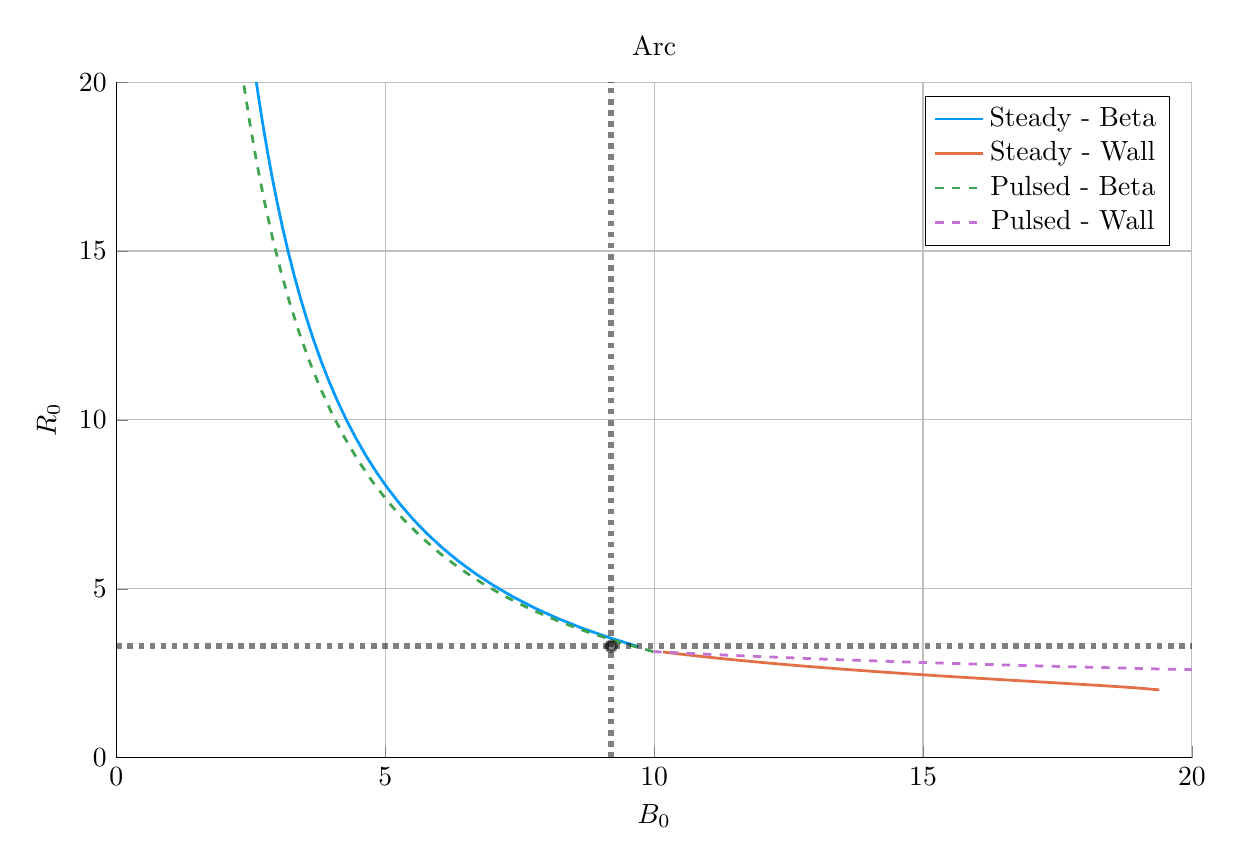
\begin{tikzpicture}[]
\begin{axis}[height = {101.6mm}, ylabel = {${R}_{0}$}, title = {Arc}, xmin = {0.0}, xmax = {20.0}, ymax = {20.0}, xlabel = {${B}_{0}$}, {unbounded coords=jump, scaled x ticks = false, xticklabel style={rotate = 0}, xmajorgrids = true, xtick = {0.0,5.0,10.0,15.0,20.0}, xticklabels = {0,5,10,15,20}, xtick align = inside, axis lines* = left, scaled y ticks = false, yticklabel style={rotate = 0}, ymajorgrids = true, ytick = {0.0,5.0,10.0,15.0,20.0}, yticklabels = {0,5,10,15,20}, ytick align = inside, axis lines* = left,     xshift = 0.0mm,
    yshift = 0.0mm,
    axis background/.style={fill={rgb,1:red,1.00000000;green,1.00000000;blue,1.00000000}}
, colorbar style={title=}}, ymin = {0.0}, width = {152.4mm}]\addplot+ [color = {rgb,1:red,0.00000000;green,0.60560316;blue,0.97868012},
draw opacity=1.0,
line width=1,
solid,mark = none,
mark size = 2.0,
mark options = {
    color = {rgb,1:red,0.00000000;green,0.00000000;blue,0.00000000}, draw opacity = 1.0,
    fill = {rgb,1:red,0.00000000;green,0.60560316;blue,0.97868012}, fill opacity = 1.0,
    line width = 1,
    rotate = 0,
    solid
}]coordinates {
(9.701206080853105, 3.2904233285656006)
(9.162315904693079, 3.553631706046861)
(8.664301107137337, 3.8315748016260343)
(8.203576462497304, 4.124583886864978)
(7.776718537485166, 4.433072975674755)
(7.380720231870917, 4.75741949036414)
(7.012886014999712, 5.097987291342331)
(6.670795005901889, 5.4551257000070565)
(6.352268997292712, 5.829168567645448)
(6.055344682097163, 6.220433393277178)
(5.778249464564785, 6.629220493040615)
(5.519380338856715, 7.05581222339423)
(5.2772854007125325, 7.500472260074458)
(5.050647625972996, 7.963444934423652)
(4.838270606140816, 8.444954628380609)
(4.639065978019038, 8.94520522910952)
(4.4520423235376105, 9.464379643936518)
(4.276295348572609, 10.002639375969222)
(4.110999177018484, 10.56012416048812)
(3.9553986195015125, 11.136951661929974)
(3.8088022956698633, 11.733217231026282)
(3.6705765055641186, 12.34899372141899)
(3.54013975965751, 12.984331364849716)
(3.4169578891619192, 13.639257703809928)
(3.30053966845824, 14.313777580345645)
(3.1904328903033052, 15.007873179535935)
(3.086220842019516, 15.721504126002731)
(2.9875191373772063, 16.45460763166718)
(2.8939728644914635, 17.207098692842226)
(2.8052540149097247, 17.97887033463821)
(2.7210591632720242, 18.7697939005645)
(2.6411073705789065, 19.579719385129263)
(2.565138287279709, 20.40847580717446)
(2.492910435164382, 21.255871621630877)
(2.4241996494611984, 22.12169516733927)
(2.3587976646588236, 23.0057151485579)
(2.296510829425685, 23.907681147764652)
(2.237158937627476, 24.827324167354146)
(2.180574163874242, 25.764357197843207)
(2.126600093288366, 26.71847581021091)
(2.075090836295778, 27.689358770027713)
(2.0259102202234582, 28.676668671060817)
(1.978931050353818, 29.68005258608471)
(1.9340344338545452, 30.69914273267572)
(1.8911091606836798, 31.733557151818793)
(1.8500511361739687, 32.78290039722107)
(1.8107628605384507, 33.846764233283025)
(1.773152951016952, 34.92472833975579)
(1.7371357028100902, 36.01636102117257)
(1.7026306853269466, 37.121219919229354)
(1.6695623706125668, 38.23885272635799)
(1.6378597911249178, 39.368797898817405)
(1.607456224302725, 40.51058536770822)
(1.5782889016090462, 41.663737246396295)
(1.5502987399539199, 42.82776853291479)
(1.5234300935954943, 44.00218780599217)
(1.4976305247952577, 45.18649791343829)
(1.4728505916614916, 46.38019665170201)
(1.4490436517578602, 47.58277743549339)
(1.4261656801829077, 48.79372995643627)
};
\addlegendentry{Steady - Beta}
\addplot+ [color = {rgb,1:red,0.88887350;green,0.43564919;blue,0.27812294},
draw opacity=1.0,
line width=1,
solid,mark = none,
mark size = 2.0,
mark options = {
    color = {rgb,1:red,0.00000000;green,0.00000000;blue,0.00000000}, draw opacity = 1.0,
    fill = {rgb,1:red,0.88887350;green,0.43564919;blue,0.27812294}, fill opacity = 1.0,
    line width = 1,
    rotate = 0,
    solid
}]coordinates {
(19.394007482712425, 2.006855814841082)
(18.932196567189358, 2.070220226465634)
(18.296989378345195, 2.1362327099649083)
(17.587029315408756, 2.2039322514902886)
(16.847882407994106, 2.272885741349308)
(16.111374502564406, 2.3427307443133163)
(15.396027314547156, 2.4132115621474344)
(14.710952688793137, 2.484165095168367)
(14.06168447794857, 2.555449485048069)
(13.450465418483889, 2.6269568263788754)
(12.877644538645335, 2.6986005527245354)
(12.342394470642008, 2.7703103261458715)
(11.843182246608265, 2.8420284550528074)
(11.376441269625893, 2.9137564749008216)
(10.944966372727551, 2.985307257194073)
(10.541663878705513, 3.056795384934831)
(10.165908182236457, 3.128148092221394)
};
\addlegendentry{Steady - Wall}
\addplot+ [color = {rgb,1:red,0.24222430;green,0.64327509;blue,0.30444865},
draw opacity=1.0,
line width=1,
dashed,mark = none,
mark size = 2.0,
mark options = {
    color = {rgb,1:red,0.00000000;green,0.00000000;blue,0.00000000}, draw opacity = 1.0,
    fill = {rgb,1:red,0.24222430;green,0.64327509;blue,0.30444865}, fill opacity = 1.0,
    line width = 1,
    rotate = 0,
    solid
}]coordinates {
(9.980483622051658, 3.1402982942956537)
(9.392786903460065, 3.3984668375583613)
(8.79273598103983, 3.7029994270206985)
(8.23820290909994, 4.029752381934837)
(7.725182218401588, 4.380005330007902)
(7.250078106370205, 4.755088191072525)
(6.80965553466646, 5.15638156809462)
(6.400998063035608, 5.585317075247801)
(6.0214713600430425, 6.043377623224966)
(5.668691517461799, 6.532097691007738)
(5.340497445229901, 7.053063624618788)
(5.034926745580058, 7.607914017422467)
(4.750194564008521, 8.198340243900201)
(4.484674995755211, 8.826087240213646)
(4.236884692979903, 9.49295465115087)
(4.00546837264544, 10.200798495308337)
(3.7891859704718387, 10.951533539957822)
(3.5869012239550364, 11.747136625739826)
(3.3975714987448393, 12.589651241396528)
(3.2202386987489797, 13.481193723261853)
(3.0540211220494466, 14.423961547290066)
(2.8981061427709687, 15.420244298711943)
(2.7517436139566023, 16.472438053930638)
(2.6142398986781377, 17.58306410230943)
(2.4849524463010138, 18.754793188384546)
(2.363284838174807, 19.990476791576892)
(2.248682232019848, 21.293187416028662)
(2.140627136740878, 22.666270490916787)
(2.038635448877246, 24.113411362836906)
(1.9422526775794744, 25.638722123308433)
(1.8510502754751532, 27.246854857488287)
(1.7646219756564088, 28.94315065234289)
(1.6825800061969869, 30.73383791051506)
(1.6045510059627948, 32.62630011975996)
(1.53017138625397, 34.629443897654504)
(1.4590817483192686, 36.754215952550474)
(1.3909197311384796, 39.01434852880224)
(1.3253102336217724, 41.42746903285954)
(1.261851128383913, 44.01681696754988)
(1.20009089049112, 46.81403058684408)
(1.1394908096975784, 49.863950342519615)
};
\addlegendentry{Pulsed - Beta}
\addplot+ [color = {rgb,1:red,0.76444018;green,0.44411178;blue,0.82429754},
draw opacity=1.0,
line width=1,
dashed,mark = none,
mark size = 2.0,
mark options = {
    color = {rgb,1:red,0.00000000;green,0.00000000;blue,0.00000000}, draw opacity = 1.0,
    fill = {rgb,1:red,0.76444018;green,0.44411178;blue,0.82429754}, fill opacity = 1.0,
    line width = 1,
    rotate = 0,
    solid
}]coordinates {
(29.27715761652869, 2.3448804182939873)
(25.4410619834368, 2.4377937236066716)
(22.158819835998365, 2.5322208586485804)
(19.342453256965573, 2.628163744265164)
(16.919364280634177, 2.7256238396687067)
(14.829378672669455, 2.8246020951898183)
(13.022412368922526, 2.9250989082568273)
(11.456617692058645, 3.0271140820266207)
(10.096901921254785, 3.1306467862637533)
(9.980483622051658, 3.1402982942956537)
};
\addlegendentry{Pulsed - Wall}
\addplot+ [color = {rgb,1:red,0.00000000;green,0.00000000;blue,0.00000000},
draw opacity=0.5,
line width=2,
dotted,mark = none,
mark size = 2.0,
mark options = {
    color = {rgb,1:red,0.00000000;green,0.00000000;blue,0.00000000}, draw opacity = 0.5,
    fill = {rgb,1:red,0.00000000;green,0.00000000;blue,0.00000000}, fill opacity = 0.5,
    line width = 1,
    rotate = 0,
    solid
},forget plot]coordinates {
(0.0, 3.3)
(20.0, 3.3)
};
\addplot+ [color = {rgb,1:red,0.00000000;green,0.00000000;blue,0.00000000},
draw opacity=0.5,
line width=2,
dotted,mark = none,
mark size = 2.0,
mark options = {
    color = {rgb,1:red,0.00000000;green,0.00000000;blue,0.00000000}, draw opacity = 0.5,
    fill = {rgb,1:red,0.00000000;green,0.00000000;blue,0.00000000}, fill opacity = 0.5,
    line width = 1,
    rotate = 0,
    solid
},forget plot]coordinates {
(9.2, 0.0)
(9.2, 20.0)
};
\addplot+[draw=none, color = {rgb,1:red,0.00000000;green,0.00000000;blue,0.00000000},
draw opacity=0.5,
line width=0,
solid,mark = *,
mark size = 2.0,
mark options = {
    color = {rgb,1:red,0.00000000;green,0.00000000;blue,0.00000000}, draw opacity = 0.5,
    fill = {rgb,1:red,0.00000000;green,0.00000000;blue,0.00000000}, fill opacity = 0.5,
    line width = 1,
    rotate = 0,
    solid
},forget plot] coordinates {
(9.2, 3.3)
};
\end{axis}

\end{tikzpicture}

    \end{adjustbox}
        \caption{$R_0$ vs $B_0$}
    \end{subfigure}
    \hfill
    \begin{subfigure}[t]{0.45\textwidth}
        \centering
    \begin{adjustbox}{width=\textwidth}
      \Large
      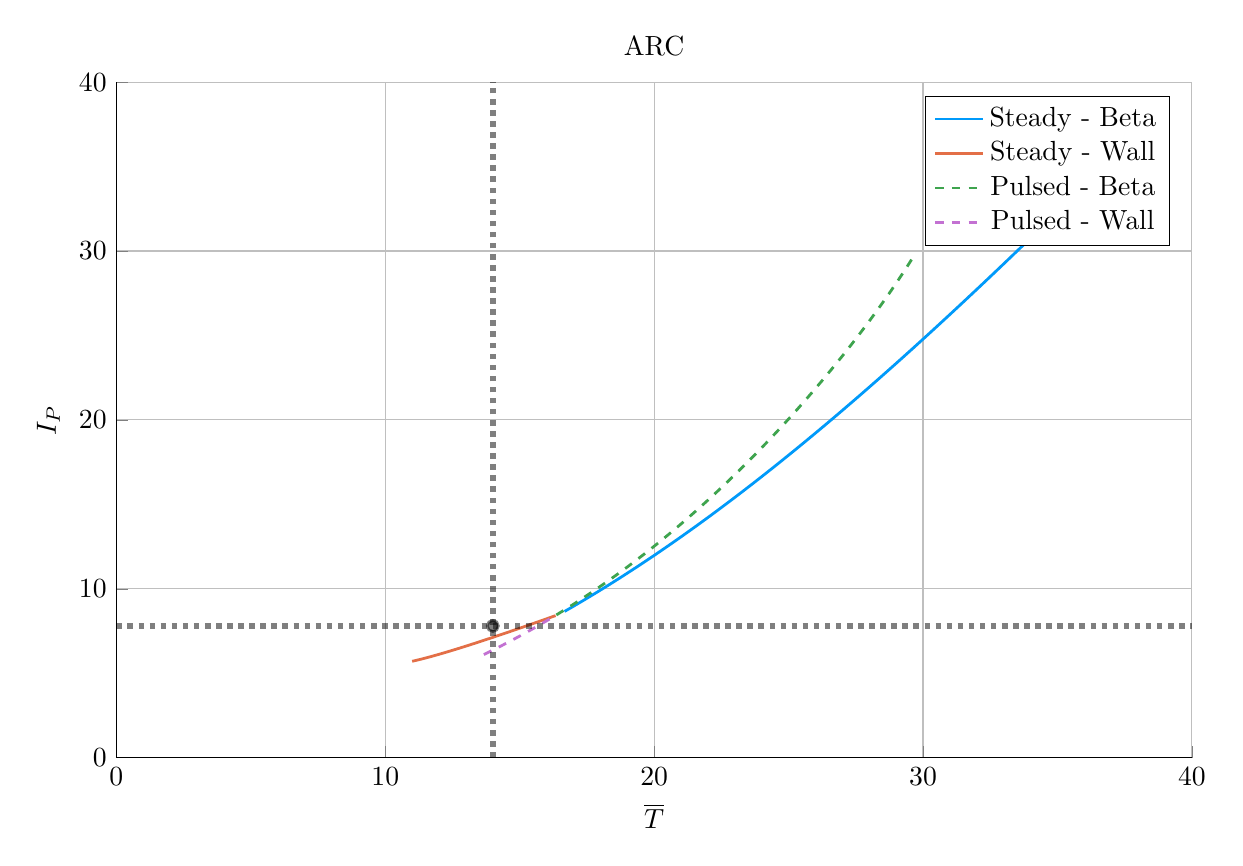
\begin{tikzpicture}[]
\begin{axis}[height = {101.6mm}, ylabel = {${I}_{P}$}, title = {ARC}, xmin = {0.0}, xmax = {40.0}, ymax = {40.0}, xlabel = {$\overline {T}$}, {unbounded coords=jump, scaled x ticks = false, xticklabel style={rotate = 0}, xmajorgrids = true, xtick = {0.0,10.0,20.0,30.0,40.0}, xticklabels = {0,10,20,30,40}, xtick align = inside, axis lines* = left, scaled y ticks = false, yticklabel style={rotate = 0}, ymajorgrids = true, ytick = {0.0,10.0,20.0,30.0,40.0}, yticklabels = {0,10,20,30,40}, ytick align = inside, axis lines* = left,     xshift = 0.0mm,
    yshift = 0.0mm,
    axis background/.style={fill={rgb,1:red,1.00000000;green,1.00000000;blue,1.00000000}}
, colorbar style={title=}}, ymin = {0.0}, width = {152.4mm}]\addplot+ [color = {rgb,1:red,0.00000000;green,0.60560316;blue,0.97868012},
draw opacity=1.0,
line width=1,
solid,mark = none,
mark size = 2.0,
mark options = {
    color = {rgb,1:red,0.00000000;green,0.00000000;blue,0.00000000}, draw opacity = 1.0,
    fill = {rgb,1:red,0.00000000;green,0.60560316;blue,0.97868012}, fill opacity = 1.0,
    line width = 1,
    rotate = 0,
    solid
}]coordinates {
(16.666666666666668, 8.658343870907427)
(17.0, 8.964855141636448)
(17.333333333333332, 9.277118721367206)
(17.666666666666668, 9.595036914426)
(18.0, 9.918585776352757)
(18.333333333333332, 10.247718935951552)
(18.666666666666668, 10.582387319200262)
(19.0, 10.922539274323045)
(19.333333333333332, 11.26812069483817)
(19.666666666666668, 11.61907514056121)
(20.0, 11.975343956529299)
(20.333333333333332, 12.336866389803589)
(20.666666666666668, 12.703579704100664)
(21.0, 13.07541929220057)
(21.333333333333332, 13.452318786079019)
(21.666666666666668, 13.834210164711733)
(22.0, 14.221023859501257)
(22.333333333333332, 14.61268885728139)
(22.666666666666668, 15.009132800857182)
(23.0, 15.410282087044596)
(23.333333333333332, 15.816061962178953)
(23.666666666666668, 16.226396615066992)
(24.0, 16.64120926736311)
(24.333333333333332, 17.060422261356294)
(24.666666666666668, 17.483957145159597)
(25.0, 17.91173475530017)
(25.333333333333332, 18.343675296712746)
(25.666666666666668, 18.77969842014449)
(26.0, 19.2197232969848)
(26.333333333333332, 19.663668691537165)
(26.666666666666668, 20.11145303075519)
(27.0, 20.562994471468567)
(27.333333333333332, 21.018210965128485)
(27.666666666666668, 21.477020320105293)
(28.0, 21.939340261574117)
(28.333333333333332, 22.405088489026962)
(28.666666666666668, 22.874182731452617)
(29.0, 23.34654080022686)
(29.333333333333332, 23.82208063975841)
(29.666666666666668, 24.300720375936947)
(30.0, 24.782378362431352)
(30.333333333333332, 25.26697322488704)
(30.666666666666668, 25.754423903072542)
(31.0, 26.244649691026318)
(31.333333333333332, 26.737570275254438)
(31.666666666666668, 27.233105771031717)
(32.0, 27.731176756857092)
(32.333333333333336, 28.23170430711659)
(32.666666666666664, 28.734610023004112)
(33.0, 29.23981606175298)
(33.333333333333336, 29.747245164229085)
(33.666666666666664, 30.256820680936514)
(34.0, 30.768466596486252)
(34.333333333333336, 31.282107552577845)
(34.666666666666664, 31.797668869543177)
(35.0, 32.31507656650066)
(35.333333333333336, 32.83425738016771)
(35.666666666666664, 33.35513878237846)
(36.0, 33.87764899635294)
(36.333333333333336, 34.40171701176134)
};
\addlegendentry{Steady - Beta}
\addplot+ [color = {rgb,1:red,0.88887350;green,0.43564919;blue,0.27812294},
draw opacity=1.0,
line width=1,
solid,mark = none,
mark size = 2.0,
mark options = {
    color = {rgb,1:red,0.00000000;green,0.00000000;blue,0.00000000}, draw opacity = 1.0,
    fill = {rgb,1:red,0.88887350;green,0.43564919;blue,0.27812294}, fill opacity = 1.0,
    line width = 1,
    rotate = 0,
    solid
}]coordinates {
(11.0, 5.705363947896813)
(11.333333333333334, 5.831631927327359)
(11.666666666666666, 5.971358416795512)
(12.0, 6.120248050030096)
(12.333333333333334, 6.27635241161913)
(12.666666666666666, 6.438084943966173)
(13.0, 6.6043437111573775)
(13.333333333333334, 6.774432932493379)
(13.666666666666666, 6.9477586358526295)
(14.0, 7.123875039246037)
(14.333333333333334, 7.302428845502918)
(14.666666666666666, 7.483135839919747)
(15.0, 7.66576464137543)
(15.333333333333334, 7.850323804140159)
(15.666666666666666, 8.036059275223955)
(16.0, 8.223435700494395)
(16.333333333333332, 8.412159667095638)
};
\addlegendentry{Steady - Wall}
\addplot+ [color = {rgb,1:red,0.24222430;green,0.64327509;blue,0.30444865},
draw opacity=1.0,
line width=1,
dashed,mark = none,
mark size = 2.0,
mark options = {
    color = {rgb,1:red,0.00000000;green,0.00000000;blue,0.00000000}, draw opacity = 1.0,
    fill = {rgb,1:red,0.24222430;green,0.64327509;blue,0.30444865}, fill opacity = 1.0,
    line width = 1,
    rotate = 0,
    solid
}]coordinates {
(16.364160609330686, 8.45211123232532)
(16.666666666666668, 8.749174237506722)
(17.0, 9.084875445329175)
(17.333333333333332, 9.429466194729264)
(17.666666666666668, 9.783065958753857)
(18.0, 10.145791398086809)
(18.333333333333332, 10.517756265001724)
(18.666666666666668, 10.899071333792335)
(19.0, 11.28984436597908)
(19.333333333333332, 11.690180120182706)
(19.666666666666668, 12.100180418434789)
(20.0, 12.519944282916168)
(20.333333333333332, 12.949568159742276)
(20.666666666666668, 13.389146249526421)
(21.0, 13.838770968145022)
(21.333333333333332, 14.298533565526986)
(21.666666666666668, 14.768524935556082)
(22.0, 15.2488366565296)
(22.333333333333332, 15.739562309352701)
(22.666666666666668, 16.240799130174846)
(23.0, 16.752650066058415)
(23.333333333333332, 17.27522631730515)
(23.666666666666668, 17.808650469386293)
(24.0, 18.353060342640163)
(24.333333333333332, 18.908613721362002)
(24.666666666666668, 19.475494169025602)
(25.0, 20.053918198206937)
(25.333333333333332, 20.644144149900036)
(25.666666666666668, 21.246483258877372)
(26.0, 21.861313557471373)
(26.333333333333332, 22.48909752802998)
(26.666666666666668, 23.130404800381292)
(27.0, 23.785941781633092)
(27.333333333333332, 24.456591033172632)
(27.666666666666668, 25.143464707502787)
(28.0, 25.84797885666414)
(28.333333333333332, 26.571959755666764)
(28.666666666666668, 27.3178012356156)
(29.0, 28.088707029156687)
(29.333333333333332, 28.889082725820668)
(29.666666666666668, 29.725209471035893)
};
\addlegendentry{Pulsed - Beta}
\addplot+ [color = {rgb,1:red,0.76444018;green,0.44411178;blue,0.82429754},
draw opacity=1.0,
line width=1,
dashed,mark = none,
mark size = 2.0,
mark options = {
    color = {rgb,1:red,0.00000000;green,0.00000000;blue,0.00000000}, draw opacity = 1.0,
    fill = {rgb,1:red,0.76444018;green,0.44411178;blue,0.82429754}, fill opacity = 1.0,
    line width = 1,
    rotate = 0,
    solid
}]coordinates {
(13.666666666666666, 6.106956435644008)
(14.0, 6.368429153074452)
(14.333333333333334, 6.637611037727747)
(14.666666666666666, 6.914640849606676)
(15.0, 7.199655680909235)
(15.333333333333334, 7.492790823032018)
(15.666666666666666, 7.794179619860046)
(16.0, 8.103953307930404)
(16.333333333333332, 8.422240844292133)
(16.364160609330686, 8.45211123232532)
};
\addlegendentry{Pulsed - Wall}
\addplot+ [color = {rgb,1:red,0.00000000;green,0.00000000;blue,0.00000000},
draw opacity=0.5,
line width=2,
dotted,mark = none,
mark size = 2.0,
mark options = {
    color = {rgb,1:red,0.00000000;green,0.00000000;blue,0.00000000}, draw opacity = 0.5,
    fill = {rgb,1:red,0.00000000;green,0.00000000;blue,0.00000000}, fill opacity = 0.5,
    line width = 1,
    rotate = 0,
    solid
},forget plot]coordinates {
(0.0, 7.8)
(40.0, 7.8)
};
\addplot+ [color = {rgb,1:red,0.00000000;green,0.00000000;blue,0.00000000},
draw opacity=0.5,
line width=2,
dotted,mark = none,
mark size = 2.0,
mark options = {
    color = {rgb,1:red,0.00000000;green,0.00000000;blue,0.00000000}, draw opacity = 0.5,
    fill = {rgb,1:red,0.00000000;green,0.00000000;blue,0.00000000}, fill opacity = 0.5,
    line width = 1,
    rotate = 0,
    solid
},forget plot]coordinates {
(14.0, 0.0)
(14.0, 40.0)
};
\addplot+[draw=none, color = {rgb,1:red,0.00000000;green,0.00000000;blue,0.00000000},
draw opacity=0.5,
line width=0,
solid,mark = *,
mark size = 2.0,
mark options = {
    color = {rgb,1:red,0.00000000;green,0.00000000;blue,0.00000000}, draw opacity = 0.5,
    fill = {rgb,1:red,0.00000000;green,0.00000000;blue,0.00000000}, fill opacity = 0.5,
    line width = 1,
    rotate = 0,
    solid
},forget plot] coordinates {
(14.0, 7.8)
};
\end{axis}

\end{tikzpicture}

    \end{adjustbox}
        \caption{$I_P$ vs $\overline T$}
    \end{subfigure}
    \hfill \hfill ~\\ ~\\ ~\\
    \caption{Arc Model Comparison} ~\\
\end{figure*}

\begin{table}[h!]
\centering  
\caption{Arc Variables}
\hfill
\begin{subtable}[t]{0.4\textwidth}
\centering  
\caption{Input Variables} ~\\
\begin{tabular}{ c|c } 

Input            & Value           \\
\hline
$H$              & 1.8             \\
$Q$              & 13.6            \\
$N_{G}$          & 0.67            \\
$\epsilon$       & 0.333          \\
$\kappa_{95}$    & 1.84            \\
$\delta_{95}$    & 0.333           \\
$\nu_{n}$        & 0.385           \\
$\nu_{T}$        & 0.929           \\
$l_{i}$          & 0.67            \\
$A$              & 2.5             \\
$Z_{eff}$        & 1.2             \\
$f_{D}$          & 0.9             \\
$\tau_{FT}$      & 1.6e9           \\
$B_{CS}$         & 12.77           \\

\end{tabular}
\end{subtable}
\hfill
\begin{subtable}[t]{0.5\textwidth}
\centering  
\caption{Output Variables} ~\\
\begin{tabular}{ c|c|c } 

Output           & Original         & Fussy.jl        \\
\hline
$R_{0}$          & 3.3              & 3.4           \\
$B_{0}$          & 9.2              & 9.5           \\
$I_{P}$          & 7.8              & 8.8           \\
$\overline n$    & 1.3              & 1.3           \\
$\overline T$    & 14.0             & 16.8           \\
$\beta_{N}$       & 0.026           & -          \\
$q_{95}$         & 7.2              & 6.1           \\
$P_{W}$          & 2.5              & 2.2           \\
$f_{BS}$         & 0.63             & 0.56          \\
$f_{CD}$         & 0.37             & 0.44          \\
$f_{IN}$         & -              & -             \\
$\volume$         & 141            & 157           \\
$P_{F}$          & 525            & 726           \\
$\eta_{CD}$      & 0.321            & 0.316          \\

\end{tabular}
\end{subtable}
\hfill
\hfill
\end{table}

\newpage

\subsection{Contrasting with the Aries Act Studies}

Moving on, the Aries Act study focuses on how steady-state reactors would look under both a conservative and optimistic perspective. This is highlighted in \cref{fig:act_h_cost}, which shows how costs decreases as the H factor is allowed to increase. Notice that for every value of H, the ACT I study (i.e. the optimistic act) has a lower cost than the design from ACT II (i.e. the conservative one).

This figure also highlights another peculiarity of the ARIES study -- a reliance on the minimum possible value of H. Note that just left of the reactor point on both plots is a highly erratic portion of the curve. As such, if even a slightly smaller value of H were used in either case, a quite distinct reactor would occur. This is not a robust way to design machines. A better approach would be to build with some safety factor -- i.e at a slightly more magical version of H. This can be seen in ARC's H-Sweep.

\begin{figure*}[h!]
    \centering
    \hfill 
    \begin{subfigure}[t]{0.4\textwidth}
        \centering
    \begin{adjustbox}{width=\textwidth}
      \Large
      \begin{tikzpicture}[]
\begin{axis}[height = {101.6mm}, ylabel = {${C}_{W}$}, title = {Act I}, xmin = {0.0}, xmax = {3.9599999999999995}, ymax = {0.1}, xlabel = {${H}$}, {unbounded coords=jump, scaled x ticks = false, xticklabel style={rotate = 0}, xmajorgrids = true, xtick = {0.0,1.0,2.0,3.0}, xticklabels = {0,1,2,3}, xtick align = inside, axis lines* = left, scaled y ticks = false, yticklabel style={rotate = 0}, ymajorgrids = true, ytick = {0.0,0.02,0.04,0.06,0.08,0.1}, yticklabels = {0.00,0.02,0.04,0.06,0.08,0.10}, ytick align = inside, axis lines* = left,     xshift = 0.0mm,
    yshift = 0.0mm,
    axis background/.style={fill={rgb,1:red,1.00000000;green,1.00000000;blue,1.00000000}}
, colorbar style={title=}}, ymin = {0.0}, width = {152.4mm}]\addplot+ [color = {rgb,1:red,0.88887350;green,0.43564919;blue,0.27812294},
draw opacity=0.7,
line width=3,
dotted,mark = none,
mark size = 2.0,
mark options = {
    color = {rgb,1:red,0.00000000;green,0.00000000;blue,0.00000000}, draw opacity = 0.7,
    fill = {rgb,1:red,0.88887350;green,0.43564919;blue,0.27812294}, fill opacity = 0.7,
    line width = 1,
    rotate = 0,
    solid
}]coordinates {
(1.65, 0.0038580882449725513)
(1.7325, 0.0034224421580344765)
(1.815, 0.0031242773601625963)
(1.8975, 0.0029076912463966475)
(1.98, 0.0027437459144664237)
(2.0625, 0.002615755758688704)
(2.145, 0.0025133725117807595)
};
\addlegendentry{$wall$}
\addplot+ [color = {rgb,1:red,0.24222430;green,0.64327509;blue,0.30444865},
draw opacity=0.7,
line width=1,
solid,mark = none,
mark size = 2.0,
mark options = {
    color = {rgb,1:red,0.00000000;green,0.00000000;blue,0.00000000}, draw opacity = 0.7,
    fill = {rgb,1:red,0.24222430;green,0.64327509;blue,0.30444865}, fill opacity = 0.7,
    line width = 1,
    rotate = 0,
    solid
}]coordinates {
(1.4025, 0.025918216479107938)
(1.485, 0.012095504772150555)
(1.5675, 0.005882239716429097)
(1.65, 0.0038447827755938714)
(1.7325, 0.0034077229105716356)
(1.815, 0.0031112188891089447)
(1.8975, 0.002896491612881698)
(1.98, 0.002734083771296579)
(2.0625, 0.002607278997942983)
(2.145, 0.002505795370579703)
(2.2275, 0.0024978293322600134)
(2.31, 0.0026050612316072053)
(2.3925, 0.002711328730788369)
(2.475, 0.0028163739703009525)
(2.5575, 0.002920119984789825)
(2.64, 0.0030223238461750735)
(2.7225, 0.003122910039550508)
(2.805, 0.003221795626029453)
(2.8875, 0.003318919864510233)
(2.97, 0.003414240640857473)
(3.0525, 0.003507731326910594)
(3.135, 0.003599378182186399)
(3.2175, 0.00368917819814934)
(3.3, 0.003777137172338829)
};
\addlegendentry{$cost$}
\addplot+ [color = {rgb,1:red,0.76444018;green,0.44411178;blue,0.82429754},
draw opacity=0.7,
line width=1,
solid,mark = none,
mark size = 2.0,
mark options = {
    color = {rgb,1:red,0.00000000;green,0.00000000;blue,0.00000000}, draw opacity = 0.7,
    fill = {rgb,1:red,0.76444018;green,0.44411178;blue,0.82429754}, fill opacity = 0.7,
    line width = 1,
    rotate = 0,
    solid
}]coordinates {
(1.4025, 0.02636776101728183)
(1.485, 0.018483166138998787)
(1.5675, 0.007170526433976295)
(1.65, 0.003841721357482374)
(1.7325, 0.0034053745614292777)
(1.815, 0.0031097242744622163)
(1.8975, 0.002895546190157591)
(1.98, 0.0027334738346990873)
(2.0625, 0.002606876408558846)
(2.145, 0.0025055240752749086)
(2.2275, 0.0024978197141057924)
(2.31, 0.0026050530799257014)
(2.3925, 0.0027113218095688846)
(2.475, 0.0028164020534254693)
(2.5575, 0.0029201149972198264)
(2.64, 0.0030223196276555316)
(2.7225, 0.003122906476745389)
(2.805, 0.0032217926032687013)
(2.8875, 0.0033189173512138603)
(2.97, 0.0034142385345432096)
(3.0525, 0.0035077295453675586)
(3.135, 0.0035993767225118564)
(3.2175, 0.003689176968945425)
(3.3, 0.0037771361544507143)
};
\addlegendentry{$W_M$}
\addplot+ [color = {rgb,1:red,0.67554396;green,0.55566233;blue,0.09423434},
draw opacity=1.0,
line width=1,
dashed,mark = none,
mark size = 2.0,
mark options = {
    color = {rgb,1:red,0.00000000;green,0.00000000;blue,0.00000000}, draw opacity = 1.0,
    fill = {rgb,1:red,0.67554396;green,0.55566233;blue,0.09423434}, fill opacity = 1.0,
    line width = 1,
    rotate = 0,
    solid
},forget plot]coordinates {
(1.65, 0.0)
(1.65, 0.1)
};
\addplot+ [color = {rgb,1:red,0.00000048;green,0.66575898;blue,0.68099695},
draw opacity=1.0,
line width=1,
dashed,mark = none,
mark size = 2.0,
mark options = {
    color = {rgb,1:red,0.00000000;green,0.00000000;blue,0.00000000}, draw opacity = 1.0,
    fill = {rgb,1:red,0.00000048;green,0.66575898;blue,0.68099695}, fill opacity = 1.0,
    line width = 1,
    rotate = 0,
    solid
},forget plot]coordinates {
(0.0, 0.0)
(0.0, 0.1)
};
\addplot+ [color = {rgb,1:red,0.00000048;green,0.66575898;blue,0.68099695},
draw opacity=1.0,
line width=1,
dashed,mark = none,
mark size = 2.0,
mark options = {
    color = {rgb,1:red,0.00000000;green,0.00000000;blue,0.00000000}, draw opacity = 1.0,
    fill = {rgb,1:red,0.00000048;green,0.66575898;blue,0.68099695}, fill opacity = 1.0,
    line width = 1,
    rotate = 0,
    solid
},forget plot]coordinates {
(3.3, 0.0)
(3.3, 0.1)
};
\end{axis}

\end{tikzpicture}

    \end{adjustbox}
        \caption{Act I H Sweep}
    \end{subfigure}
    \hfill
    \begin{subfigure}[t]{0.4\textwidth}
        \centering
    \begin{adjustbox}{width=\textwidth}
      \Large
      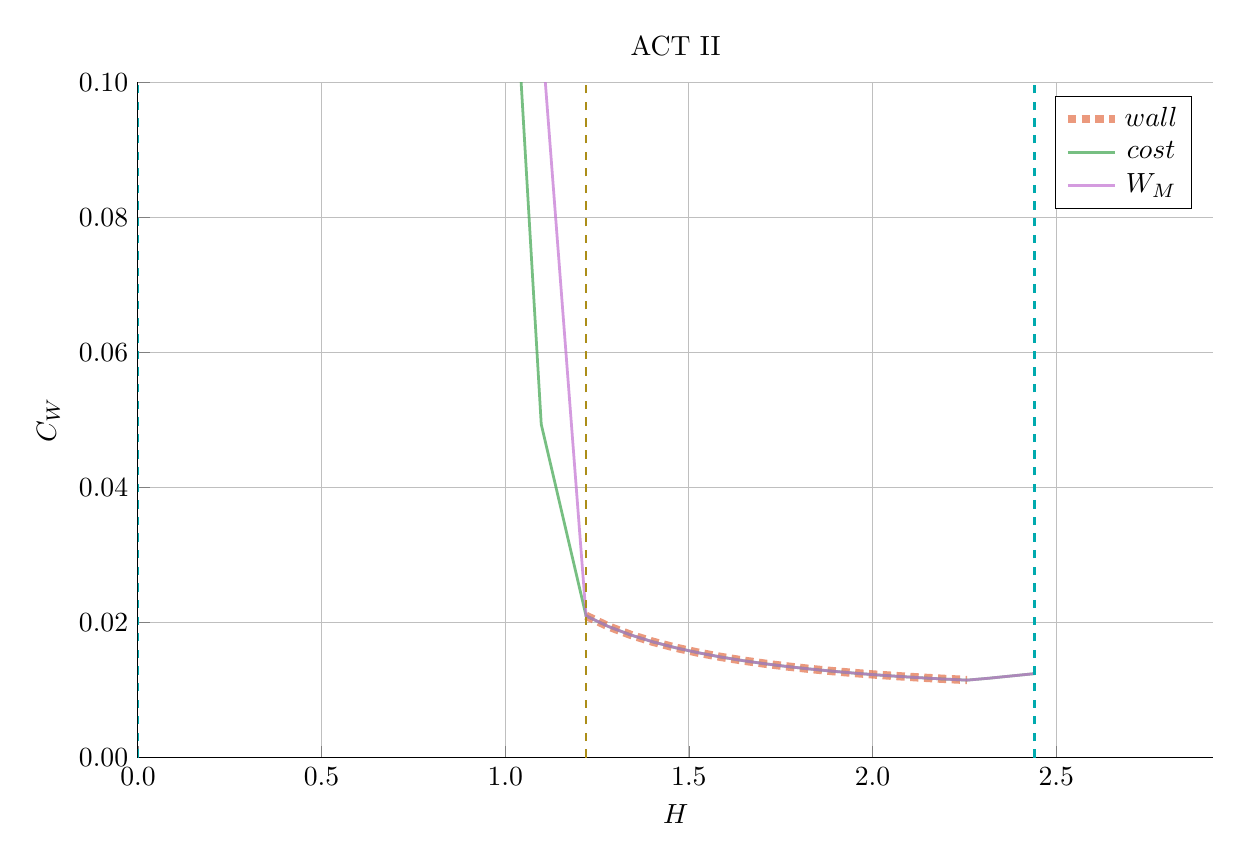
\begin{tikzpicture}[]
\begin{axis}[height = {101.6mm}, ylabel = {${C}_{W}$}, title = {ACT II}, xmin = {0.0}, xmax = {2.928}, ymax = {0.1}, xlabel = {${H}$}, {unbounded coords=jump, scaled x ticks = false, xticklabel style={rotate = 0}, xmajorgrids = true, xtick = {0.0,0.5,1.0,1.5,2.0,2.5}, xticklabels = {0.0,0.5,1.0,1.5,2.0,2.5}, xtick align = inside, axis lines* = left, scaled y ticks = false, yticklabel style={rotate = 0}, ymajorgrids = true, ytick = {0.0,0.02,0.04,0.06,0.08,0.1}, yticklabels = {0.00,0.02,0.04,0.06,0.08,0.10}, ytick align = inside, axis lines* = left,     xshift = 0.0mm,
    yshift = 0.0mm,
    axis background/.style={fill={rgb,1:red,1.00000000;green,1.00000000;blue,1.00000000}}
, colorbar style={title=}}, ymin = {0.0}, width = {152.4mm}]\addplot+ [color = {rgb,1:red,0.88887350;green,0.43564919;blue,0.27812294},
draw opacity=0.7,
line width=3,
dotted,mark = none,
mark size = 2.0,
mark options = {
    color = {rgb,1:red,0.00000000;green,0.00000000;blue,0.00000000}, draw opacity = 0.7,
    fill = {rgb,1:red,0.88887350;green,0.43564919;blue,0.27812294}, fill opacity = 0.7,
    line width = 1,
    rotate = 0,
    solid
}]coordinates {
(1.22, 0.021005512518330174)
(1.281, 0.01942744270360855)
(1.342, 0.018170389811630824)
(1.403, 0.017139710886836464)
(1.464, 0.01627794436788193)
(1.525, 0.015546450836866612)
(1.586, 0.014919600022944367)
(1.647, 0.014377436937475022)
(1.708, 0.013905581766222853)
(1.769, 0.01349265356023887)
(1.83, 0.013129558656358339)
(1.891, 0.01280891244140467)
(1.952, 0.012524569645508304)
(2.013, 0.01227184717788876)
(2.074, 0.012046102834086084)
(2.135, 0.01184360516877147)
(2.196, 0.011661349792575638)
(2.257, 0.011496773538316084)
};
\addlegendentry{$wall$}
\addplot+ [color = {rgb,1:red,0.24222430;green,0.64327509;blue,0.30444865},
draw opacity=0.7,
line width=1,
solid,mark = none,
mark size = 2.0,
mark options = {
    color = {rgb,1:red,0.00000000;green,0.00000000;blue,0.00000000}, draw opacity = 0.7,
    fill = {rgb,1:red,0.24222430;green,0.64327509;blue,0.30444865}, fill opacity = 0.7,
    line width = 1,
    rotate = 0,
    solid
}]coordinates {
(1.037, 0.10576482650233505)
(1.098, 0.04935829436307264)
(1.22, 0.020990970199014802)
(1.281, 0.0194129595370893)
(1.342, 0.01815662533322952)
(1.403, 0.01712672739309554)
(1.464, 0.016265578765863785)
(1.525, 0.015534719386234706)
(1.586, 0.014908297877268767)
(1.647, 0.014366575271189693)
(1.708, 0.013895114510245749)
(1.769, 0.013482541510434981)
(1.83, 0.013119766959557726)
(1.891, 0.012796621459369077)
(1.952, 0.012503284271399288)
(2.013, 0.012246990247871287)
(2.074, 0.012019443303647051)
(2.135, 0.011815835760118812)
(2.196, 0.011632962604193957)
(2.257, 0.011474758216077388)
(2.318, 0.011765579200211946)
(2.379, 0.012101340215422274)
(2.44, 0.012432978177363389)
};
\addlegendentry{$cost$}
\addplot+ [color = {rgb,1:red,0.76444018;green,0.44411178;blue,0.82429754},
draw opacity=0.7,
line width=1,
solid,mark = none,
mark size = 2.0,
mark options = {
    color = {rgb,1:red,0.00000000;green,0.00000000;blue,0.00000000}, draw opacity = 0.7,
    fill = {rgb,1:red,0.76444018;green,0.44411178;blue,0.82429754}, fill opacity = 0.7,
    line width = 1,
    rotate = 0,
    solid
}]coordinates {
(1.098, 0.10789687618345375)
(1.22, 0.020993563020398034)
(1.281, 0.019414381524971283)
(1.342, 0.018157569810455732)
(1.403, 0.017127496371177657)
(1.464, 0.016266077641847662)
(1.525, 0.015535219465132215)
(1.586, 0.014908546212398566)
(1.647, 0.014366740003006752)
(1.708, 0.013895218421357018)
(1.769, 0.01348260263682947)
(1.83, 0.013119799308255348)
(1.891, 0.0127993859843838)
(1.952, 0.012506614611284711)
(2.013, 0.01224686415179682)
(2.074, 0.012019222925033022)
(2.135, 0.011815568425293648)
(2.196, 0.011632678053496345)
(2.257, 0.011474127813480542)
(2.318, 0.011765572318494604)
(2.379, 0.012101333413489)
(2.44, 0.012432971811628111)
};
\addlegendentry{$W_M$}
\addplot+ [color = {rgb,1:red,0.67554396;green,0.55566233;blue,0.09423434},
draw opacity=1.0,
line width=1,
dashed,mark = none,
mark size = 2.0,
mark options = {
    color = {rgb,1:red,0.00000000;green,0.00000000;blue,0.00000000}, draw opacity = 1.0,
    fill = {rgb,1:red,0.67554396;green,0.55566233;blue,0.09423434}, fill opacity = 1.0,
    line width = 1,
    rotate = 0,
    solid
},forget plot]coordinates {
(1.22, 0.0)
(1.22, 0.1)
};
\addplot+ [color = {rgb,1:red,0.00000048;green,0.66575898;blue,0.68099695},
draw opacity=1.0,
line width=1,
dashed,mark = none,
mark size = 2.0,
mark options = {
    color = {rgb,1:red,0.00000000;green,0.00000000;blue,0.00000000}, draw opacity = 1.0,
    fill = {rgb,1:red,0.00000048;green,0.66575898;blue,0.68099695}, fill opacity = 1.0,
    line width = 1,
    rotate = 0,
    solid
},forget plot]coordinates {
(0.0, 0.0)
(0.0, 0.1)
};
\addplot+ [color = {rgb,1:red,0.00000048;green,0.66575898;blue,0.68099695},
draw opacity=1.0,
line width=1,
dashed,mark = none,
mark size = 2.0,
mark options = {
    color = {rgb,1:red,0.00000000;green,0.00000000;blue,0.00000000}, draw opacity = 1.0,
    fill = {rgb,1:red,0.00000048;green,0.66575898;blue,0.68099695}, fill opacity = 1.0,
    line width = 1,
    rotate = 0,
    solid
},forget plot]coordinates {
(2.44, 0.0)
(2.44, 0.1)
};
\end{axis}

\end{tikzpicture}

    \end{adjustbox}
        \caption{Act II H Sweep}
    \end{subfigure}
    \hfill \hfill ~\\ ~\\ ~\\
    \begin{subfigure}[t]{0.4\textwidth}
        \centering
		\begin{adjustbox}{width=\textwidth}
			\Large
			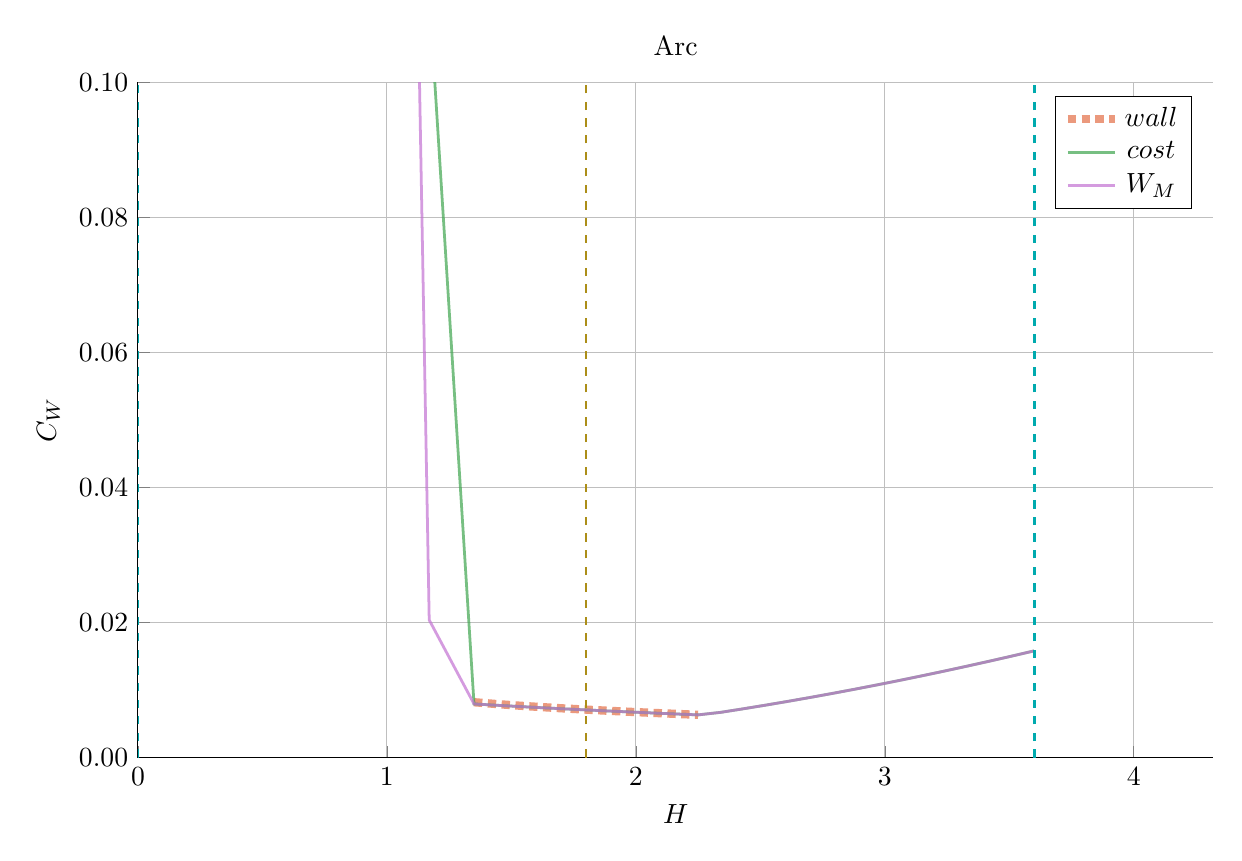
\begin{tikzpicture}[]
\begin{axis}[height = {101.6mm}, ylabel = {${C}_{W}$}, title = {Arc}, xmin = {0.0}, xmax = {4.32}, ymax = {0.1}, xlabel = {${H}$}, {unbounded coords=jump, scaled x ticks = false, xticklabel style={rotate = 0}, xmajorgrids = true, xtick = {0.0,1.0,2.0,3.0,4.0}, xticklabels = {0,1,2,3,4}, xtick align = inside, axis lines* = left, scaled y ticks = false, yticklabel style={rotate = 0}, ymajorgrids = true, ytick = {0.0,0.02,0.04,0.06,0.08,0.1}, yticklabels = {0.00,0.02,0.04,0.06,0.08,0.10}, ytick align = inside, axis lines* = left,     xshift = 0.0mm,
    yshift = 0.0mm,
    axis background/.style={fill={rgb,1:red,1.00000000;green,1.00000000;blue,1.00000000}}
, colorbar style={title=}}, ymin = {0.0}, width = {152.4mm}]\addplot+ [color = {rgb,1:red,0.88887350;green,0.43564919;blue,0.27812294},
draw opacity=0.7,
line width=3,
dotted,mark = none,
mark size = 2.0,
mark options = {
    color = {rgb,1:red,0.00000000;green,0.00000000;blue,0.00000000}, draw opacity = 0.7,
    fill = {rgb,1:red,0.88887350;green,0.43564919;blue,0.27812294}, fill opacity = 0.7,
    line width = 1,
    rotate = 0,
    solid
}]coordinates {
(1.35, 0.008207241762396246)
(1.44, 0.00793667759257354)
(1.53, 0.0076997912429461225)
(1.62, 0.007486816554981894)
(1.71, 0.007291648689881567)
(1.8, 0.007110333347796811)
(1.89, 0.006940248814588952)
(1.98, 0.006779633349026309)
(2.07, 0.006627297197584387)
(2.16, 0.006482438866566955)
(2.25, 0.006344768968841929)
};
\addlegendentry{$wall$}
\addplot+ [color = {rgb,1:red,0.24222430;green,0.64327509;blue,0.30444865},
draw opacity=0.7,
line width=1,
solid,mark = none,
mark size = 2.0,
mark options = {
    color = {rgb,1:red,0.00000000;green,0.00000000;blue,0.00000000}, draw opacity = 0.7,
    fill = {rgb,1:red,0.24222430;green,0.64327509;blue,0.30444865}, fill opacity = 0.7,
    line width = 1,
    rotate = 0,
    solid
}]coordinates {
(1.08, 0.1656933786109522)
(1.35, 0.007956028922350611)
(1.44, 0.007759662745290108)
(1.53, 0.007574913322065527)
(1.62, 0.00739885086770846)
(1.71, 0.0072297906534508185)
(1.8, 0.007066784363464752)
(1.89, 0.00690932755478892)
(1.98, 0.006757201835765392)
(2.07, 0.006610359300650354)
(2.16, 0.0064688545800951625)
(2.25, 0.006332913629979953)
(2.34, 0.00670268792962123)
(2.43, 0.0072243580642261445)
(2.52, 0.007766406785339575)
(2.61, 0.008328785580854575)
(2.7, 0.008911412315791628)
(2.79, 0.00951417119398493)
(2.88, 0.010136912409268534)
(2.97, 0.010779452862615483)
(3.06, 0.011441576670944502)
(3.15, 0.012123036438828786)
(3.24, 0.012823554577929932)
(3.33, 0.0135428254017145)
(3.42, 0.014280516598644705)
(3.51, 0.015036271676563144)
(3.6, 0.01580971210009804)
};
\addlegendentry{$cost$}
\addplot+ [color = {rgb,1:red,0.76444018;green,0.44411178;blue,0.82429754},
draw opacity=0.7,
line width=1,
solid,mark = none,
mark size = 2.0,
mark options = {
    color = {rgb,1:red,0.00000000;green,0.00000000;blue,0.00000000}, draw opacity = 0.7,
    fill = {rgb,1:red,0.76444018;green,0.44411178;blue,0.82429754}, fill opacity = 0.7,
    line width = 1,
    rotate = 0,
    solid
}]coordinates {
(1.08, 0.20419403931121408)
(1.17, 0.02038194154635263)
(1.35, 0.007952462446561684)
(1.44, 0.007756882763096937)
(1.53, 0.007572765485693452)
(1.62, 0.007397214242173672)
(1.71, 0.007228584574974498)
(1.8, 0.007065962995902896)
(1.89, 0.006908746287963411)
(1.98, 0.006756833824238413)
(2.07, 0.0066101524637499)
(2.16, 0.006468686518064958)
(2.25, 0.006332754951862069)
(2.34, 0.00670262687626648)
(2.43, 0.007224172350640052)
(2.52, 0.007766066748915404)
(2.61, 0.008328266004035769)
(2.7, 0.008910694013555907)
(2.79, 0.009513241975770496)
(2.88, 0.010135768084513136)
(2.97, 0.010778097603257038)
(3.06, 0.011440023505553681)
(3.15, 0.01212130721887041)
(3.24, 0.012821680052634414)
(3.33, 0.013540844476435391)
(3.42, 0.014278476232750113)
(3.51, 0.015034225935616565)
(3.6, 0.01580772161808181)
};
\addlegendentry{$W_M$}
\addplot+ [color = {rgb,1:red,0.67554396;green,0.55566233;blue,0.09423434},
draw opacity=1.0,
line width=1,
dashed,mark = none,
mark size = 2.0,
mark options = {
    color = {rgb,1:red,0.00000000;green,0.00000000;blue,0.00000000}, draw opacity = 1.0,
    fill = {rgb,1:red,0.67554396;green,0.55566233;blue,0.09423434}, fill opacity = 1.0,
    line width = 1,
    rotate = 0,
    solid
},forget plot]coordinates {
(1.8, 0.0)
(1.8, 0.1)
};
\addplot+ [color = {rgb,1:red,0.00000048;green,0.66575898;blue,0.68099695},
draw opacity=1.0,
line width=1,
dashed,mark = none,
mark size = 2.0,
mark options = {
    color = {rgb,1:red,0.00000000;green,0.00000000;blue,0.00000000}, draw opacity = 1.0,
    fill = {rgb,1:red,0.00000048;green,0.66575898;blue,0.68099695}, fill opacity = 1.0,
    line width = 1,
    rotate = 0,
    solid
},forget plot]coordinates {
(0.0, 0.0)
(0.0, 0.1)
};
\addplot+ [color = {rgb,1:red,0.00000048;green,0.66575898;blue,0.68099695},
draw opacity=1.0,
line width=1,
dashed,mark = none,
mark size = 2.0,
mark options = {
    color = {rgb,1:red,0.00000000;green,0.00000000;blue,0.00000000}, draw opacity = 1.0,
    fill = {rgb,1:red,0.00000048;green,0.66575898;blue,0.68099695}, fill opacity = 1.0,
    line width = 1,
    rotate = 0,
    solid
},forget plot]coordinates {
(3.6, 0.0)
(3.6, 0.1)
};
\end{axis}

\end{tikzpicture}

		\end{adjustbox}
        \caption{Arc H Sweep}
    \end{subfigure} ~\\ ~\\ ~\\
    \caption{Act Studies Cost Dependence on the H Factor} ~\\    
	\label{fig:act_h_cost}
\end{figure*}

\newpage 

\subsubsection{Act I -- Advanced Physics and Engineering}

Act 1 is the ARIES study that assumes advanced physics and engineering design parameters. Although this paper's model does a good job matching the results from their paper, it does show what optimistic design really means. As can be seen, this design actually only surpasses the minimum possible toroidal field strength by as less than a Tesla! Practically, this means the reactor is barely realizable.

\begin{figure*}[h!]
    \centering
    \hfill 
    \begin{subfigure}[t]{0.45\textwidth}
        \centering
    \begin{adjustbox}{width=\textwidth}
      \Large
      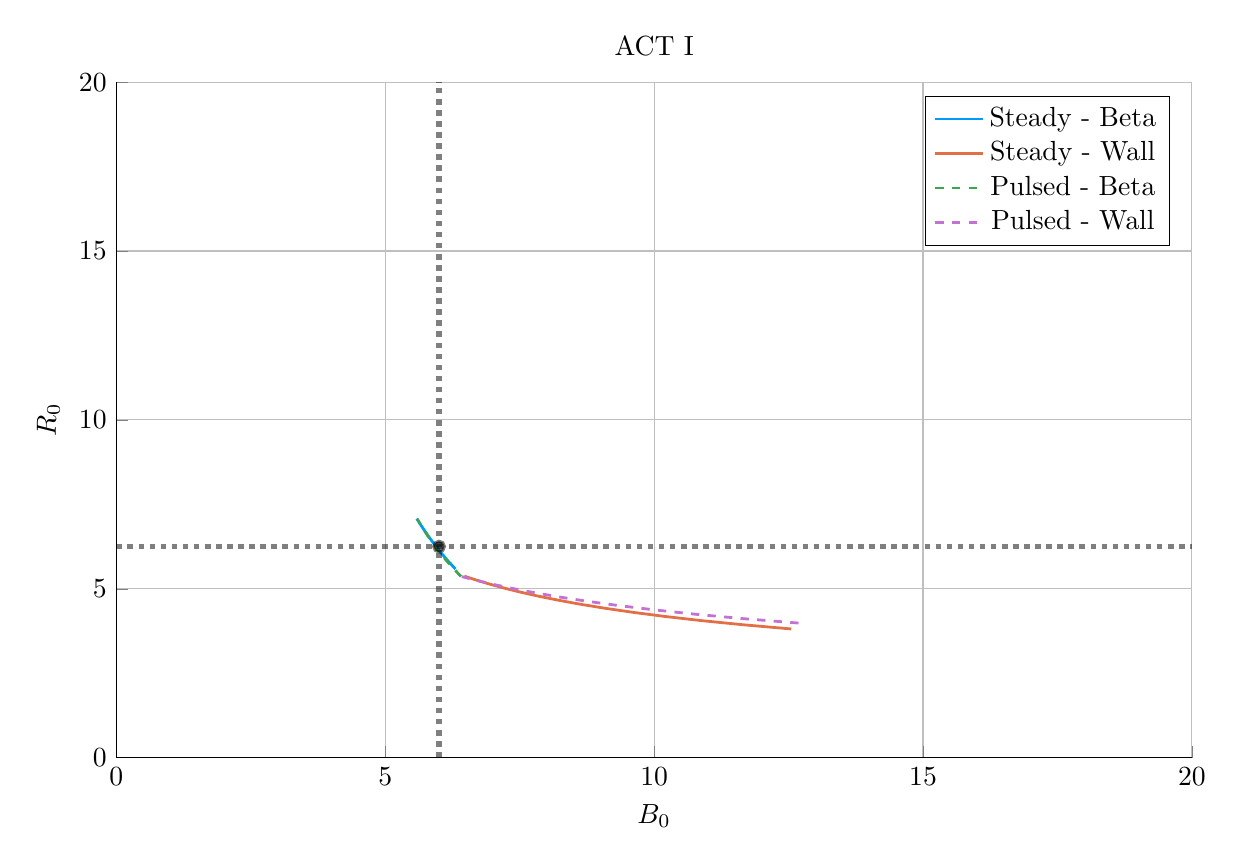
\begin{tikzpicture}[]
\begin{axis}[height = {101.6mm}, ylabel = {${R}_{0}$}, title = {ACT I}, xmin = {0.0}, xmax = {20.0}, ymax = {20.0}, xlabel = {${B}_{0}$}, {unbounded coords=jump, scaled x ticks = false, xticklabel style={rotate = 0}, xmajorgrids = true, xtick = {0.0,5.0,10.0,15.0,20.0}, xticklabels = {0,5,10,15,20}, xtick align = inside, axis lines* = left, scaled y ticks = false, yticklabel style={rotate = 0}, ymajorgrids = true, ytick = {0.0,5.0,10.0,15.0,20.0}, yticklabels = {0,5,10,15,20}, ytick align = inside, axis lines* = left,     xshift = 0.0mm,
    yshift = 0.0mm,
    axis background/.style={fill={rgb,1:red,1.00000000;green,1.00000000;blue,1.00000000}}
, colorbar style={title=}}, ymin = {0.0}, width = {152.4mm}]\addplot+ [color = {rgb,1:red,0.00000000;green,0.60560316;blue,0.97868012},
draw opacity=1.0,
line width=1,
solid,mark = none,
mark size = 2.0,
mark options = {
    color = {rgb,1:red,0.00000000;green,0.00000000;blue,0.00000000}, draw opacity = 1.0,
    fill = {rgb,1:red,0.00000000;green,0.60560316;blue,0.97868012}, fill opacity = 1.0,
    line width = 1,
    rotate = 0,
    solid
}]coordinates {
(6.30336807958207, 5.587199391496101)
(6.162193069273141, 5.831838137107903)
(6.030717178404645, 6.078157823726375)
(5.908065509576601, 6.325994353145188)
(5.793464904530972, 6.57518910191267)
(5.686229631357383, 6.825588847053452)
(5.585749511271037, 7.077045564754442)
};
\addlegendentry{Steady - Beta}
\addplot+ [color = {rgb,1:red,0.88887350;green,0.43564919;blue,0.27812294},
draw opacity=1.0,
line width=1,
solid,mark = none,
mark size = 2.0,
mark options = {
    color = {rgb,1:red,0.00000000;green,0.00000000;blue,0.00000000}, draw opacity = 1.0,
    fill = {rgb,1:red,0.88887350;green,0.43564919;blue,0.27812294}, fill opacity = 1.0,
    line width = 1,
    rotate = 0,
    solid
}]coordinates {
(12.549536249695134, 3.8108352245940957)
(11.658754653696462, 3.934083270736017)
(10.883719833507003, 4.057046546594516)
(10.206258129789394, 4.179626810883221)
(9.611335769312953, 4.301750356443285)
(9.086446934250878, 4.423366229113912)
(8.62129895070743, 4.544434218016914)
(8.207216040989662, 4.6649335402400025)
(7.837119555085499, 4.78484200403474)
(7.505047858717157, 4.9041467319817595)
(7.20604322925957, 5.022835870779136)
(6.935884710193303, 5.1409045607718795)
(6.691016583192173, 5.258349129805506)
(6.468415485086983, 5.375167957409874)
};
\addlegendentry{Steady - Wall}
\addplot+ [color = {rgb,1:red,0.24222430;green,0.64327509;blue,0.30444865},
draw opacity=1.0,
line width=1,
dashed,mark = none,
mark size = 2.0,
mark options = {
    color = {rgb,1:red,0.00000000;green,0.00000000;blue,0.00000000}, draw opacity = 1.0,
    fill = {rgb,1:red,0.24222430;green,0.64327509;blue,0.30444865}, fill opacity = 1.0,
    line width = 1,
    rotate = 0,
    solid
}]coordinates {
(6.408263337806559, 5.366131328829866)
(6.408263337806564, 5.366131328829862)
(6.385466513301022, 5.402805883604879)
(6.245492502072912, 5.638974714472524)
(6.116010320461132, 5.875875066688821)
(5.9960421481916395, 6.113307727774442)
(5.884727159112828, 6.351082733498888)
(5.781304768121868, 6.589019058920955)
(5.685100648450046, 6.826944315253105)
(5.595515000321003, 7.064694456596427)
};
\addlegendentry{Pulsed - Beta}
\addplot+ [color = {rgb,1:red,0.76444018;green,0.44411178;blue,0.82429754},
draw opacity=1.0,
line width=1,
dashed,mark = none,
mark size = 2.0,
mark options = {
    color = {rgb,1:red,0.00000000;green,0.00000000;blue,0.00000000}, draw opacity = 1.0,
    fill = {rgb,1:red,0.76444018;green,0.44411178;blue,0.82429754}, fill opacity = 1.0,
    line width = 1,
    rotate = 0,
    solid
}]coordinates {
(12.684248532650473, 3.9847907768802657)
(11.66307871570063, 4.114684512780648)
(10.781888309639141, 4.244124103742294)
(10.016282491385791, 4.373086052625054)
(9.346943280276514, 4.501549309887817)
(8.758420158941194, 4.6294950281779785)
(8.238241792953433, 4.756906348757686)
(7.776255600865612, 4.883768212546736)
(7.364131118520045, 5.010067192354689)
(6.994982564641668, 5.135791343697217)
(6.66307916140573, 5.260930071474144)
(6.408263337806559, 5.366131328829866)
(6.408263337806564, 5.366131328829862)
};
\addlegendentry{Pulsed - Wall}
\addplot+ [color = {rgb,1:red,0.00000000;green,0.00000000;blue,0.00000000},
draw opacity=0.5,
line width=2,
dotted,mark = none,
mark size = 2.0,
mark options = {
    color = {rgb,1:red,0.00000000;green,0.00000000;blue,0.00000000}, draw opacity = 0.5,
    fill = {rgb,1:red,0.00000000;green,0.00000000;blue,0.00000000}, fill opacity = 0.5,
    line width = 1,
    rotate = 0,
    solid
},forget plot]coordinates {
(0.0, 6.25)
(20.0, 6.25)
};
\addplot+ [color = {rgb,1:red,0.00000000;green,0.00000000;blue,0.00000000},
draw opacity=0.5,
line width=2,
dotted,mark = none,
mark size = 2.0,
mark options = {
    color = {rgb,1:red,0.00000000;green,0.00000000;blue,0.00000000}, draw opacity = 0.5,
    fill = {rgb,1:red,0.00000000;green,0.00000000;blue,0.00000000}, fill opacity = 0.5,
    line width = 1,
    rotate = 0,
    solid
},forget plot]coordinates {
(6.0, 0.0)
(6.0, 20.0)
};
\addplot+[draw=none, color = {rgb,1:red,0.00000000;green,0.00000000;blue,0.00000000},
draw opacity=0.5,
line width=0,
solid,mark = *,
mark size = 2.0,
mark options = {
    color = {rgb,1:red,0.00000000;green,0.00000000;blue,0.00000000}, draw opacity = 0.5,
    fill = {rgb,1:red,0.00000000;green,0.00000000;blue,0.00000000}, fill opacity = 0.5,
    line width = 1,
    rotate = 0,
    solid
},forget plot] coordinates {
(6.0, 6.25)
};
\end{axis}

\end{tikzpicture}

    \end{adjustbox}
        \caption{$R_0$ vs $B_0$}
    \end{subfigure}
    \hfill
    \begin{subfigure}[t]{0.45\textwidth}
        \centering
    \begin{adjustbox}{width=\textwidth}
      \Large
      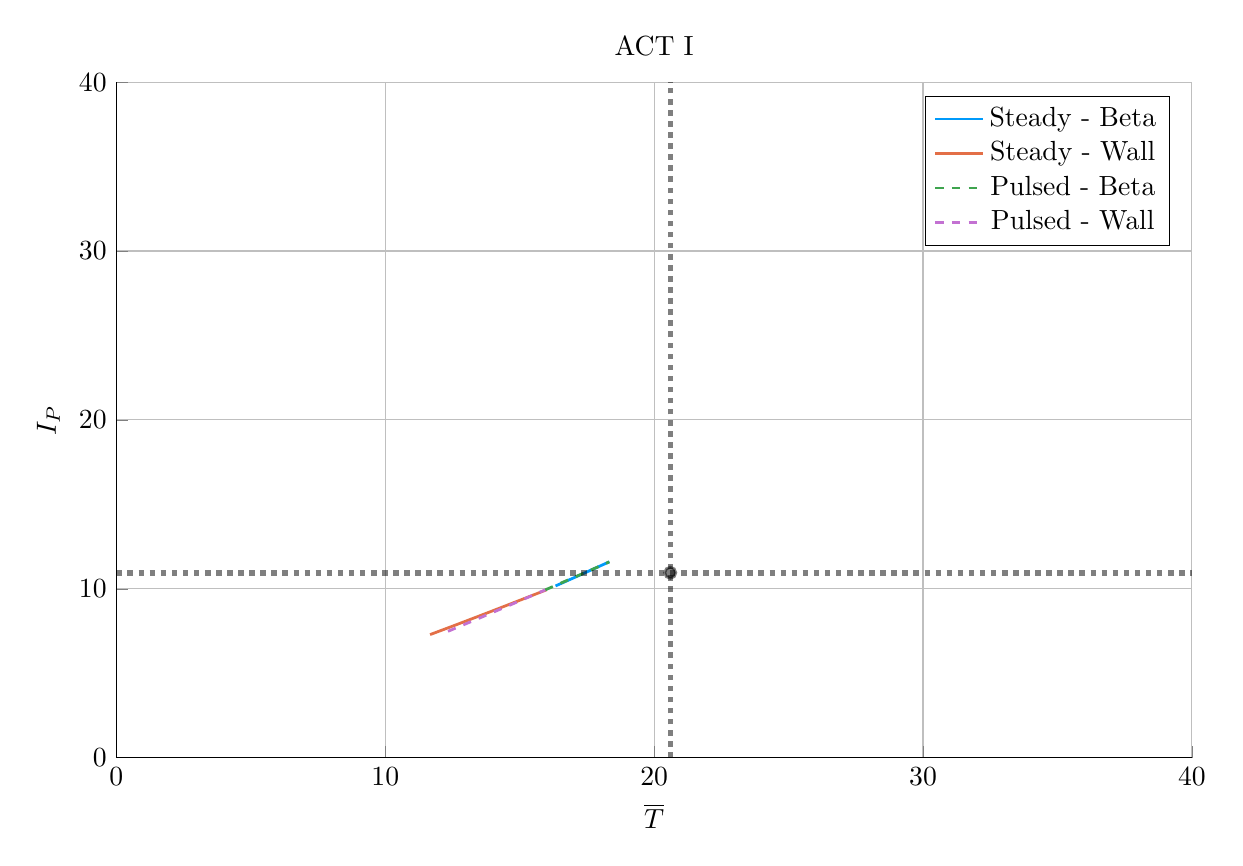
\begin{tikzpicture}[]
\begin{axis}[height = {101.6mm}, ylabel = {${I}_{P}$}, title = {ACT I}, xmin = {0.0}, xmax = {40.0}, ymax = {40.0}, xlabel = {$\overline {T}$}, {unbounded coords=jump, scaled x ticks = false, xticklabel style={rotate = 0}, xmajorgrids = true, xtick = {0.0,10.0,20.0,30.0,40.0}, xticklabels = {0,10,20,30,40}, xtick align = inside, axis lines* = left, scaled y ticks = false, yticklabel style={rotate = 0}, ymajorgrids = true, ytick = {0.0,10.0,20.0,30.0,40.0}, yticklabels = {0,10,20,30,40}, ytick align = inside, axis lines* = left,     xshift = 0.0mm,
    yshift = 0.0mm,
    axis background/.style={fill={rgb,1:red,1.00000000;green,1.00000000;blue,1.00000000}}
, colorbar style={title=}}, ymin = {0.0}, width = {152.4mm}]\addplot+ [color = {rgb,1:red,0.00000000;green,0.60560316;blue,0.97868012},
draw opacity=1.0,
line width=1,
solid,mark = none,
mark size = 2.0,
mark options = {
    color = {rgb,1:red,0.00000000;green,0.00000000;blue,0.00000000}, draw opacity = 1.0,
    fill = {rgb,1:red,0.00000000;green,0.60560316;blue,0.97868012}, fill opacity = 1.0,
    line width = 1,
    rotate = 0,
    solid
}]coordinates {
(16.333333333333332, 10.169194435531358)
(16.666666666666668, 10.405057509328124)
(17.0, 10.641905327194731)
(17.333333333333332, 10.87971637136811)
(17.666666666666668, 11.11846917050157)
(18.0, 11.358142407296011)
(18.333333333333332, 11.598714938197329)
};
\addlegendentry{Steady - Beta}
\addplot+ [color = {rgb,1:red,0.88887350;green,0.43564919;blue,0.27812294},
draw opacity=1.0,
line width=1,
solid,mark = none,
mark size = 2.0,
mark options = {
    color = {rgb,1:red,0.00000000;green,0.00000000;blue,0.00000000}, draw opacity = 1.0,
    fill = {rgb,1:red,0.88887350;green,0.43564919;blue,0.27812294}, fill opacity = 1.0,
    line width = 1,
    rotate = 0,
    solid
}]coordinates {
(11.666666666666666, 7.287903136887)
(12.0, 7.486025430610099)
(12.333333333333334, 7.685696663157812)
(12.666666666666666, 7.886645361110723)
(13.0, 8.08866940687473)
(13.333333333333334, 8.291629426976055)
(13.666666666666666, 8.495414075666067)
(14.0, 8.699964056113311)
(14.333333333333334, 8.905213556979005)
(14.666666666666666, 9.111120468746519)
(15.0, 9.31764336053339)
(15.333333333333334, 9.524758318501357)
(15.666666666666666, 9.732442959434447)
(16.0, 9.940679052729761)
};
\addlegendentry{Steady - Wall}
\addplot+ [color = {rgb,1:red,0.24222430;green,0.64327509;blue,0.30444865},
draw opacity=1.0,
line width=1,
dashed,mark = none,
mark size = 2.0,
mark options = {
    color = {rgb,1:red,0.00000000;green,0.00000000;blue,0.00000000}, draw opacity = 1.0,
    fill = {rgb,1:red,0.24222430;green,0.64327509;blue,0.30444865}, fill opacity = 1.0,
    line width = 1,
    rotate = 0,
    solid
}]coordinates {
(15.948125117373092, 9.933500150990564)
(15.9481251173731, 9.933500150990564)
(16.0, 9.969282740147014)
(16.333333333333332, 10.199548426407084)
(16.666666666666668, 10.430379144484162)
(17.0, 10.661750348679098)
(17.333333333333332, 10.893638132753678)
(17.666666666666668, 11.126019229767902)
(18.0, 11.358871009413285)
(18.333333333333332, 11.592171473618816)
};
\addlegendentry{Pulsed - Beta}
\addplot+ [color = {rgb,1:red,0.76444018;green,0.44411178;blue,0.82429754},
draw opacity=1.0,
line width=1,
dashed,mark = none,
mark size = 2.0,
mark options = {
    color = {rgb,1:red,0.00000000;green,0.00000000;blue,0.00000000}, draw opacity = 1.0,
    fill = {rgb,1:red,0.76444018;green,0.44411178;blue,0.82429754}, fill opacity = 1.0,
    line width = 1,
    rotate = 0,
    solid
}]coordinates {
(12.333333333333334, 7.481290856821823)
(12.666666666666666, 7.703549290655078)
(13.0, 7.92668121689452)
(13.333333333333334, 8.15065615613957)
(13.666666666666666, 8.375443966327172)
(14.0, 8.601014900773066)
(14.333333333333334, 8.82733966430566)
(14.666666666666666, 9.054389459546684)
(15.0, 9.282136024328327)
(15.333333333333334, 9.510551661584085)
(15.666666666666666, 9.73960926266661)
(15.948125117373092, 9.933500150990564)
(15.9481251173731, 9.933500150990564)
};
\addlegendentry{Pulsed - Wall}
\addplot+ [color = {rgb,1:red,0.00000000;green,0.00000000;blue,0.00000000},
draw opacity=0.5,
line width=2,
dotted,mark = none,
mark size = 2.0,
mark options = {
    color = {rgb,1:red,0.00000000;green,0.00000000;blue,0.00000000}, draw opacity = 0.5,
    fill = {rgb,1:red,0.00000000;green,0.00000000;blue,0.00000000}, fill opacity = 0.5,
    line width = 1,
    rotate = 0,
    solid
},forget plot]coordinates {
(0.0, 10.95)
(40.0, 10.95)
};
\addplot+ [color = {rgb,1:red,0.00000000;green,0.00000000;blue,0.00000000},
draw opacity=0.5,
line width=2,
dotted,mark = none,
mark size = 2.0,
mark options = {
    color = {rgb,1:red,0.00000000;green,0.00000000;blue,0.00000000}, draw opacity = 0.5,
    fill = {rgb,1:red,0.00000000;green,0.00000000;blue,0.00000000}, fill opacity = 0.5,
    line width = 1,
    rotate = 0,
    solid
},forget plot]coordinates {
(20.6, 0.0)
(20.6, 40.0)
};
\addplot+[draw=none, color = {rgb,1:red,0.00000000;green,0.00000000;blue,0.00000000},
draw opacity=0.5,
line width=0,
solid,mark = *,
mark size = 2.0,
mark options = {
    color = {rgb,1:red,0.00000000;green,0.00000000;blue,0.00000000}, draw opacity = 0.5,
    fill = {rgb,1:red,0.00000000;green,0.00000000;blue,0.00000000}, fill opacity = 0.5,
    line width = 1,
    rotate = 0,
    solid
},forget plot] coordinates {
(20.6, 10.95)
};
\end{axis}

\end{tikzpicture}

    \end{adjustbox}
        \caption{$I_P$ vs $\overline T$}
    \end{subfigure}
    \hfill \hfill ~\\ ~\\ ~\\
    \caption{Aries Act I Model Comparison} ~\\
\end{figure*}

\begin{table}[h!]
\centering  
\caption{Act I Variables}
\hfill
\begin{subtable}[t]{0.4\textwidth}
\centering  
\caption{Input Variables} ~\\
\begin{tabular}{ c|c } 

Input            & Value           \\
\hline
$H$              & 1.65            \\
$Q$              & 42.5            \\
$N_{G}$          & 1.0             \\
$\epsilon$       & 0.25            \\
$\kappa_{95}$    & 2.1             \\
$\delta_{95}$    & 0.4             \\
$\nu_{n}$        & 0.27            \\
$\nu_{T}$        & 1.15            \\
$l_{i}$          & 0.359         \\
$A$              & 2.5             \\
$Z_{eff}$        & 2.11            \\
$f_{D}$          & 0.75            \\
$\tau_{FT}$      & 1.6e9           \\
$B_{CS}$         & 12.77           \\

\end{tabular}
\end{subtable}
\hfill
\begin{subtable}[t]{0.5\textwidth}
\centering  
\caption{Output Variables} ~\\
\begin{tabular}{ c|c|c } 

Output           & Original         & Fussy.jl        \\
\hline
$R_{0}$          & 6.25             & 6.23           \\
$B_{0}$          & 6.0              & 6.0           \\
$I_{P}$          & 10.95            & 10.78           \\
$\overline n$    & 1.3              & 1.3           \\
$\overline T$    & 20.6             & 17.2            \\
$\beta_{N}$       & 0.0427           & -          \\
$q_{95}$         & 4.5              & 4.0           \\
$P_{W}$          & 2.45             & 2.00           \\
$f_{BS}$         & 0.91             & 0.91           \\
$f_{CD}$         & 0.09             & 0.09           \\
$f_{IN}$         & -              & -             \\
$\volume$         & 582.0            & 621.4           \\
$P_{F}$          & 1813           & 1865          \\
$\eta_{CD}$      & 0.188            & 0.185          \\

\end{tabular}
\end{subtable}
\hfill
\hfill
\end{table}

\newpage 

\subsubsection{Act II -- Conservative Physics and Engineering}

ARIES more conservative design -- Act II -- is much more like ARC in nature. From the plots, its obvious the paper's model is basically right on top of the reactor curve made using Fussy.jl.  Much like ARC, too, it shows how the model overestimates fusion power and underestimates bootstrap fraction due to the selection of a pedestal profile for plasma temperature.

\begin{figure*}[h!]
    \centering
    \hfill 
    \begin{subfigure}[t]{0.45\textwidth}
        \centering
    \begin{adjustbox}{width=\textwidth}
      \Large
      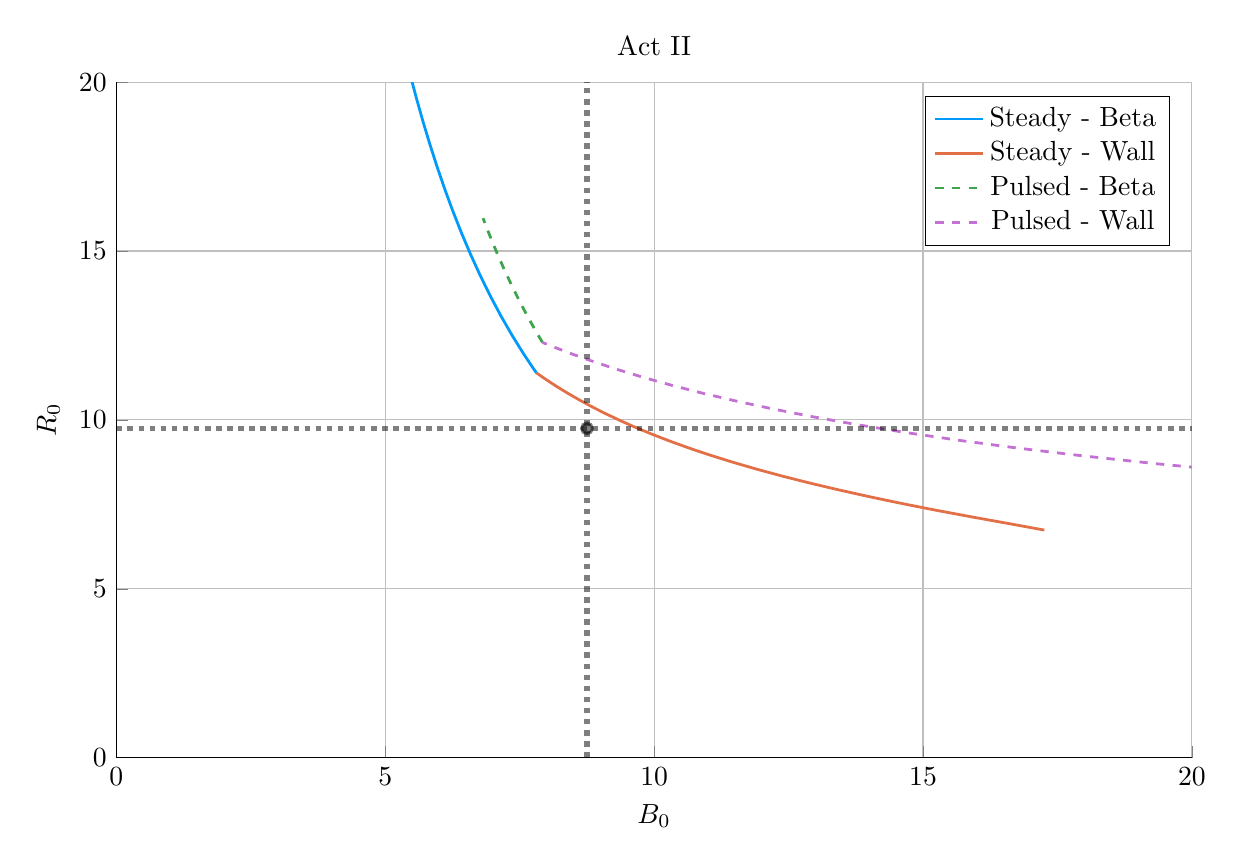
\begin{tikzpicture}[]
\begin{axis}[height = {101.6mm}, ylabel = {${R}_{0}$}, title = {Act II}, xmin = {0.0}, xmax = {20.0}, ymax = {20.0}, xlabel = {${B}_{0}$}, {unbounded coords=jump, scaled x ticks = false, xticklabel style={rotate = 0}, xmajorgrids = true, xtick = {0.0,5.0,10.0,15.0,20.0}, xticklabels = {0,5,10,15,20}, xtick align = inside, axis lines* = left, scaled y ticks = false, yticklabel style={rotate = 0}, ymajorgrids = true, ytick = {0.0,5.0,10.0,15.0,20.0}, yticklabels = {0,5,10,15,20}, ytick align = inside, axis lines* = left,     xshift = 0.0mm,
    yshift = 0.0mm,
    axis background/.style={fill={rgb,1:red,1.00000000;green,1.00000000;blue,1.00000000}}
, colorbar style={title=}}, ymin = {0.0}, width = {152.4mm}]\addplot+ [color = {rgb,1:red,0.00000000;green,0.60560316;blue,0.97868012},
draw opacity=1.0,
line width=1,
solid,mark = none,
mark size = 2.0,
mark options = {
    color = {rgb,1:red,0.00000000;green,0.00000000;blue,0.00000000}, draw opacity = 1.0,
    fill = {rgb,1:red,0.00000000;green,0.60560316;blue,0.97868012}, fill opacity = 1.0,
    line width = 1,
    rotate = 0,
    solid
}]coordinates {
(7.810935944285959, 11.389141268081966)
(7.57736049850867, 11.942634046586162)
(7.354864292609041, 12.51245847357923)
(7.145167234136329, 13.0943365692581)
(6.9473303865083675, 13.687993788149779)
(6.760499508614096, 14.293145886478186)
(6.583897990324067, 14.909495325365516)
(6.416817229618043, 15.536734694045393)
(6.258609820663305, 16.1745467994937)
(6.108683264880386, 16.82260538899235)
(5.966494431410919, 17.480575868750975)
(5.831544666176381, 18.148116014600475)
(5.703375459679132, 18.824876684423757)
(5.581564609582325, 19.510502502077443)
(5.465722802994068, 20.20463254880097)
(5.355490573482678, 20.906901035327614)
(5.25053558682053, 21.616937949657327)
(5.1505502068221745, 22.334369714080776)
(5.0552493196883175, 23.058819802110854)
};
\addlegendentry{Steady - Beta}
\addplot+ [color = {rgb,1:red,0.88887350;green,0.43564919;blue,0.27812294},
draw opacity=1.0,
line width=1,
solid,mark = none,
mark size = 2.0,
mark options = {
    color = {rgb,1:red,0.00000000;green,0.00000000;blue,0.00000000}, draw opacity = 1.0,
    fill = {rgb,1:red,0.88887350;green,0.43564919;blue,0.27812294}, fill opacity = 1.0,
    line width = 1,
    rotate = 0,
    solid
}]coordinates {
(17.25550839059296, 6.738604635617289)
(16.594334962335296, 6.931178286222189)
(15.9071755430688, 7.128187388035985)
(15.233983138507648, 7.327817939330552)
(14.594239858921854, 7.528927553154291)
(13.989673082630297, 7.7312042898700515)
(13.414782495717416, 7.934790159202381)
(12.872659546281994, 8.139273115071695)
(12.364365715508608, 8.344321605506495)
(11.889507953196574, 8.549679244077495)
(11.44685939646348, 8.755144058838903)
(11.034739998180656, 8.960554762148757)
(10.651252523287319, 9.165781242855727)
(10.294428800132035, 9.370717743724994)
(9.962319203963213, 9.57527782549947)
(9.653045819449929, 9.779390564591205)
(9.364832254395445, 9.982997628553138)
(9.096018465506306, 10.186050992034668)
(8.844373144802077, 10.388606525997883)
(8.61055754360846, 10.590345571972314)
(8.391192178573277, 10.791527736428888)
(8.18577947665566, 10.992035979756642)
(7.99323348423048, 11.1918525509058)
(7.812301489248497, 11.391007917726574)
};
\addlegendentry{Steady - Wall}
\addplot+ [color = {rgb,1:red,0.24222430;green,0.64327509;blue,0.30444865},
draw opacity=1.0,
line width=1,
dashed,mark = none,
mark size = 2.0,
mark options = {
    color = {rgb,1:red,0.00000000;green,0.00000000;blue,0.00000000}, draw opacity = 1.0,
    fill = {rgb,1:red,0.24222430;green,0.64327509;blue,0.30444865}, fill opacity = 1.0,
    line width = 1,
    rotate = 0,
    solid
}]coordinates {
(7.923668284887995, 12.293879059492616)
(7.923668284887995, 12.293879059492635)
(7.836759696043437, 12.52591633746021)
(7.6662731560983355, 13.00454403942661)
(7.50499428233835, 13.488375025456907)
(7.35232773269976, 13.977065733125242)
(7.207727224738343, 14.470269937628656)
(7.070690693175276, 14.967639476613451)
(6.940756001029682, 15.46882496625731)
(6.817497143644154, 15.973476480630131)
};
\addlegendentry{Pulsed - Beta}
\addplot+ [color = {rgb,1:red,0.76444018;green,0.44411178;blue,0.82429754},
draw opacity=1.0,
line width=1,
dashed,mark = none,
mark size = 2.0,
mark options = {
    color = {rgb,1:red,0.00000000;green,0.00000000;blue,0.00000000}, draw opacity = 1.0,
    fill = {rgb,1:red,0.76444018;green,0.44411178;blue,0.82429754}, fill opacity = 1.0,
    line width = 1,
    rotate = 0,
    solid
}]coordinates {
(22.56106430311702, 8.239911323116141)
(20.85607192394036, 8.471453471694678)
(19.335265246056654, 8.703260993170346)
(17.974121547130903, 8.935277031603567)
(16.751976718553127, 9.167446093344447)
(15.651329744019142, 9.399714010238458)
(14.65728744097675, 9.632027927077594)
(13.757118584462601, 9.864336290607328)
(12.939893642194303, 10.096588839007167)
(12.196191964860315, 10.328736591776112)
(11.517862472405039, 10.560731839999896)
(10.897827027335556, 10.792528137074703)
(10.329918077124672, 11.02408028901105)
(9.808743940706389, 11.255344346143936)
(9.329576544487265, 11.486277593626015)
(8.888257451278507, 11.716838542453242)
(8.481118883411932, 11.946986920205564)
(8.10491708701527, 12.17668366154026)
(7.923668284887995, 12.293879059492616)
(7.923668284887995, 12.293879059492635)
};
\addlegendentry{Pulsed - Wall}
\addplot+ [color = {rgb,1:red,0.00000000;green,0.00000000;blue,0.00000000},
draw opacity=0.5,
line width=2,
dotted,mark = none,
mark size = 2.0,
mark options = {
    color = {rgb,1:red,0.00000000;green,0.00000000;blue,0.00000000}, draw opacity = 0.5,
    fill = {rgb,1:red,0.00000000;green,0.00000000;blue,0.00000000}, fill opacity = 0.5,
    line width = 1,
    rotate = 0,
    solid
},forget plot]coordinates {
(0.0, 9.75)
(20.0, 9.75)
};
\addplot+ [color = {rgb,1:red,0.00000000;green,0.00000000;blue,0.00000000},
draw opacity=0.5,
line width=2,
dotted,mark = none,
mark size = 2.0,
mark options = {
    color = {rgb,1:red,0.00000000;green,0.00000000;blue,0.00000000}, draw opacity = 0.5,
    fill = {rgb,1:red,0.00000000;green,0.00000000;blue,0.00000000}, fill opacity = 0.5,
    line width = 1,
    rotate = 0,
    solid
},forget plot]coordinates {
(8.75, 0.0)
(8.75, 20.0)
};
\addplot+[draw=none, color = {rgb,1:red,0.00000000;green,0.00000000;blue,0.00000000},
draw opacity=0.5,
line width=0,
solid,mark = *,
mark size = 2.0,
mark options = {
    color = {rgb,1:red,0.00000000;green,0.00000000;blue,0.00000000}, draw opacity = 0.5,
    fill = {rgb,1:red,0.00000000;green,0.00000000;blue,0.00000000}, fill opacity = 0.5,
    line width = 1,
    rotate = 0,
    solid
},forget plot] coordinates {
(8.75, 9.75)
};
\end{axis}

\end{tikzpicture}

    \end{adjustbox}
        \caption{$R_0$ vs $B_0$}
    \end{subfigure}
    \hfill
    \begin{subfigure}[t]{0.45\textwidth}
        \centering
    \begin{adjustbox}{width=\textwidth}
      \Large
      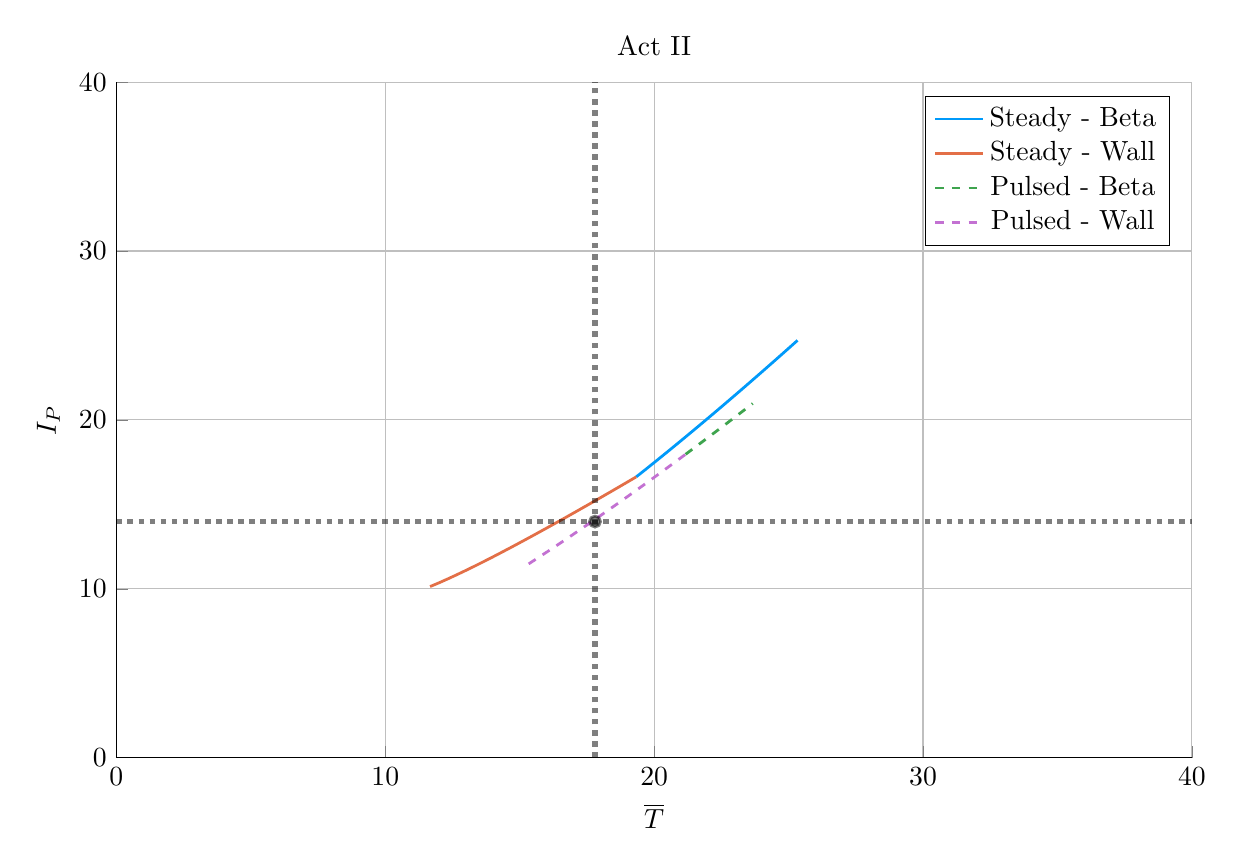
\begin{tikzpicture}[]
\begin{axis}[height = {101.6mm}, ylabel = {${I}_{P}$}, title = {Act II}, xmin = {0.0}, xmax = {40.0}, ymax = {40.0}, xlabel = {$\overline {T}$}, {unbounded coords=jump, scaled x ticks = false, xticklabel style={rotate = 0}, xmajorgrids = true, xtick = {0.0,10.0,20.0,30.0,40.0}, xticklabels = {0,10,20,30,40}, xtick align = inside, axis lines* = left, scaled y ticks = false, yticklabel style={rotate = 0}, ymajorgrids = true, ytick = {0.0,10.0,20.0,30.0,40.0}, yticklabels = {0,10,20,30,40}, ytick align = inside, axis lines* = left,     xshift = 0.0mm,
    yshift = 0.0mm,
    axis background/.style={fill={rgb,1:red,1.00000000;green,1.00000000;blue,1.00000000}}
, colorbar style={title=}}, ymin = {0.0}, width = {152.4mm}]\addplot+ [color = {rgb,1:red,0.00000000;green,0.60560316;blue,0.97868012},
draw opacity=1.0,
line width=1,
solid,mark = none,
mark size = 2.0,
mark options = {
    color = {rgb,1:red,0.00000000;green,0.00000000;blue,0.00000000}, draw opacity = 1.0,
    fill = {rgb,1:red,0.00000000;green,0.60560316;blue,0.97868012}, fill opacity = 1.0,
    line width = 1,
    rotate = 0,
    solid
}]coordinates {
(19.333333333333332, 16.626976584120992)
(19.666666666666668, 17.04714126565062)
(20.0, 17.4728205159228)
(20.333333333333332, 17.902037802268676)
(20.666666666666668, 18.334710756318135)
(21.0, 18.770758343299946)
(21.333333333333332, 19.21009903030823)
(21.666666666666668, 19.652652028291016)
(22.0, 20.098337062332053)
(22.333333333333332, 20.547074418426956)
(22.666666666666668, 20.998784986741654)
(23.0, 21.453390301179443)
(23.333333333333332, 21.910812577709113)
(23.666666666666668, 22.37097474604109)
(24.0, 22.833800482195542)
(24.333333333333332, 23.299214237115898)
(24.666666666666668, 23.767141260842724)
(25.0, 24.237507628970306)
(25.333333333333332, 24.710240262329886)
};
\addlegendentry{Steady - Beta}
\addplot+ [color = {rgb,1:red,0.88887350;green,0.43564919;blue,0.27812294},
draw opacity=1.0,
line width=1,
solid,mark = none,
mark size = 2.0,
mark options = {
    color = {rgb,1:red,0.00000000;green,0.00000000;blue,0.00000000}, draw opacity = 1.0,
    fill = {rgb,1:red,0.88887350;green,0.43564919;blue,0.27812294}, fill opacity = 1.0,
    line width = 1,
    rotate = 0,
    solid
}]coordinates {
(11.666666666666666, 10.131702672149428)
(12.0, 10.354462623384137)
(12.333333333333334, 10.591104956642406)
(12.666666666666666, 10.837356598740662)
(13.0, 11.09054386610192)
(13.333333333333334, 11.349883742416331)
(13.666666666666666, 11.61561327802365)
(14.0, 11.886764241828663)
(14.333333333333334, 12.16256217004895)
(14.666666666666666, 12.44240841774136)
(15.0, 12.72583049098312)
(15.333333333333334, 13.012449288635679)
(15.666666666666666, 13.301956539143166)
(16.0, 13.59409872387861)
(16.333333333333332, 13.888665310111481)
(16.666666666666668, 14.185479949266789)
(17.0, 14.48439377498311)
(17.333333333333332, 14.785280223642218)
(17.666666666666668, 15.088238807947413)
(18.0, 15.392552774473998)
(18.333333333333332, 15.698764813772398)
(18.666666666666668, 16.00659672680533)
(19.0, 16.315986303185774)
(19.333333333333332, 16.626976584120992)
};
\addlegendentry{Steady - Wall}
\addplot+ [color = {rgb,1:red,0.24222430;green,0.64327509;blue,0.30444865},
draw opacity=1.0,
line width=1,
dashed,mark = none,
mark size = 2.0,
mark options = {
    color = {rgb,1:red,0.00000000;green,0.00000000;blue,0.00000000}, draw opacity = 1.0,
    fill = {rgb,1:red,0.24222430;green,0.64327509;blue,0.30444865}, fill opacity = 1.0,
    line width = 1,
    rotate = 0,
    solid
}]coordinates {
(21.17034352159018, 17.96627417153032)
(21.170343521590212, 17.966274171530337)
(21.333333333333332, 18.1591936305205)
(21.666666666666668, 18.555297107283753)
(22.0, 18.953426399022014)
(22.333333333333332, 19.353497539767794)
(22.666666666666668, 19.7554274455778)
(23.0, 20.159133974954596)
(23.333333333333332, 20.564535986760628)
(23.666666666666668, 20.971553389451927)
};
\addlegendentry{Pulsed - Beta}
\addplot+ [color = {rgb,1:red,0.76444018;green,0.44411178;blue,0.82429754},
draw opacity=1.0,
line width=1,
dashed,mark = none,
mark size = 2.0,
mark options = {
    color = {rgb,1:red,0.00000000;green,0.00000000;blue,0.00000000}, draw opacity = 1.0,
    fill = {rgb,1:red,0.76444018;green,0.44411178;blue,0.82429754}, fill opacity = 1.0,
    line width = 1,
    rotate = 0,
    solid
}]coordinates {
(15.333333333333334, 11.474678053719876)
(15.666666666666666, 11.819475032994422)
(16.0, 12.167858357397087)
(16.333333333333332, 12.51974460671026)
(16.666666666666668, 12.875049128346197)
(17.0, 13.233686175102404)
(17.333333333333332, 13.595569077154208)
(17.666666666666668, 13.96061040317257)
(18.0, 14.328722110173729)
(18.333333333333332, 14.699815683529526)
(18.666666666666668, 15.073802268415148)
(19.0, 15.450592793824576)
(19.333333333333332, 15.830098089115069)
(19.666666666666668, 16.21222899561205)
(20.0, 16.596896471191773)
(20.333333333333332, 16.984011690059134)
(20.666666666666668, 17.37348613728185)
(21.0, 17.765231698435688)
(21.17034352159018, 17.96627417153032)
(21.170343521590212, 17.966274171530337)
};
\addlegendentry{Pulsed - Wall}
\addplot+ [color = {rgb,1:red,0.00000000;green,0.00000000;blue,0.00000000},
draw opacity=0.5,
line width=2,
dotted,mark = none,
mark size = 2.0,
mark options = {
    color = {rgb,1:red,0.00000000;green,0.00000000;blue,0.00000000}, draw opacity = 0.5,
    fill = {rgb,1:red,0.00000000;green,0.00000000;blue,0.00000000}, fill opacity = 0.5,
    line width = 1,
    rotate = 0,
    solid
},forget plot]coordinates {
(0.0, 13.98)
(40.0, 13.98)
};
\addplot+ [color = {rgb,1:red,0.00000000;green,0.00000000;blue,0.00000000},
draw opacity=0.5,
line width=2,
dotted,mark = none,
mark size = 2.0,
mark options = {
    color = {rgb,1:red,0.00000000;green,0.00000000;blue,0.00000000}, draw opacity = 0.5,
    fill = {rgb,1:red,0.00000000;green,0.00000000;blue,0.00000000}, fill opacity = 0.5,
    line width = 1,
    rotate = 0,
    solid
},forget plot]coordinates {
(17.8, 0.0)
(17.8, 40.0)
};
\addplot+[draw=none, color = {rgb,1:red,0.00000000;green,0.00000000;blue,0.00000000},
draw opacity=0.5,
line width=0,
solid,mark = *,
mark size = 2.0,
mark options = {
    color = {rgb,1:red,0.00000000;green,0.00000000;blue,0.00000000}, draw opacity = 0.5,
    fill = {rgb,1:red,0.00000000;green,0.00000000;blue,0.00000000}, fill opacity = 0.5,
    line width = 1,
    rotate = 0,
    solid
},forget plot] coordinates {
(17.8, 13.98)
};
\end{axis}

\end{tikzpicture}

    \end{adjustbox}
        \caption{$I_P$ vs $\overline T$}
    \end{subfigure}
    \hfill \hfill ~\\ ~\\ ~\\
    \caption{Aries Act II Model Comparison} ~\\
\end{figure*}

\begin{table}[h!]
\centering  
\caption{Act II Variables}
\hfill
\begin{subtable}[t]{0.4\textwidth}
\centering  
\caption{Input Variables} ~\\
\begin{tabular}{ c|c } 

Input            & Value           \\
\hline
$H$              & 1.22            \\
$Q$              & 25.0            \\
$N_{G}$          & 1.3             \\
$\epsilon$       & 0.25            \\
$\kappa_{95}$    & 1.964           \\
$\delta_{95}$    & 0.42            \\
$\nu_{n}$        & 0.41            \\
$\nu_{T}$        & 1.15            \\
$l_{i}$          & 0.60275         \\
$A$              & 2.5             \\
$Z_{eff}$        & 2.12            \\
$f_{D}$          & 0.74            \\
$\tau_{FT}$      & 1.6e9           \\
$B_{CS}$         & 12.77           \\

\end{tabular}
\end{subtable}
\hfill
\begin{subtable}[t]{0.5\textwidth}
\centering  
\caption{Output Variables} ~\\
\begin{tabular}{ c|c|c } 

Output           & Original         & Fussy.jl        \\
\hline
$R_{0}$          & 9.75             & 10.22           \\
$B_{0}$          & 8.75             & 9.05           \\
$I_{P}$          & 13.98            & 14.84           \\
$\overline n$    & 0.86             & 0.82          \\
$\overline T$    & 17.8             & 17.4           \\
$\beta_{N}$       & 0.026            & 0.023          \\
$q_{95}$         & 8.0              & 6.6           \\
$P_{W}$          & 1.46             & -            \\
$f_{BS}$         & 0.77             & 0.66           \\
$f_{CD}$         & 0.23             & 0.34           \\
$f_{IN}$         & -              & -             \\
$\volume$         & 2209           & 2559          \\
$P_{F}$          & 2637           & 3460          \\
$\eta_{CD}$      & 0.256            & 0.307           \\

\end{tabular}
\end{subtable}
\hfill
\hfill
\end{table}

\newpage

\subsection{Benchmarking with the Process DEMO Designs}

The PROCESS team's prospective designs for successors to ITER constitute the final set of model comparisons: the steady-state and pulsed DEMO reactors. As this paper is designed to compare these modes of operation, this study proves most fruitful. It also highlights how common model decisions can dramatically alter what reactors come out of the solvers.

The first discrepancy is how the PROCESS team defines the loss term in the ELMy H-Mode scaling law. As shown in their paper, they actually subtract out a Bremsstrahlung component, while leaving the fitting coefficients the same. \cite{process} After modifying Fussy.jl to incorporate this definition, the steady-state reactor is easily reproducible in $R_0$ -- $B_0$ slice of reactor space.

Unlike the steady-state cause, however, the modified power loss term does not fix the pulsed case, as it actually draws the reactor curves further from the design from their paper. As such, it is flux balance that is now the main source of discrepancy between the two models. This makes sense, as this model uses highly simplified source terms -- namely neglecting anything but the central solenoid and PF coils (as well as ignoring crucial physics for these two components).

Even acknowledging the differences between the two models, Fussy.jl still does remarkably well at reproducing their much more sophisticated coding framework. The final point to make is about selecting optimum points to build as the floating variables are allowed to make curves through reactor space. Up to this point, only steady-state tokamak designs have been explored. In every single one of these, the paper values have been very close to the point where the beta curves and wall loading curves cross. This is because they all result in the minimum cost-per-watt. 

For pulsed designs, on the other hand, kink curves start to appear for low magnetic field strengths. Just as beta-wall intersections were optimum places to design for low cost-per-watt ($C_W$) reactors, these beta-kink intersections will prove to be the place where minimum capital cost ($W_M$) reactors usually occur.

\newpage 

\subsubsection{DEMO Steady -- A Steady-State ITER Successor}

Hands down, this DEMO Steady reactor is the worst modeled reactor using Fussy.jl. As mentioned previously, though, some of the discrepancy was removed by using the PROCESS team's modified version of heat loss. This heavily corrected the $R_0$ -- $B_0$ curve, but had no effect on the $I_P$ -- $\overline T$ one. An interesting aside, these curves actually show that the steady current is independent of secondary constraint (as discussed).

\begin{figure*}[h!]
    \centering
    \hfill 
    \begin{subfigure}[t]{0.45\textwidth}
        \centering
    \begin{adjustbox}{width=\textwidth}
      \Large
      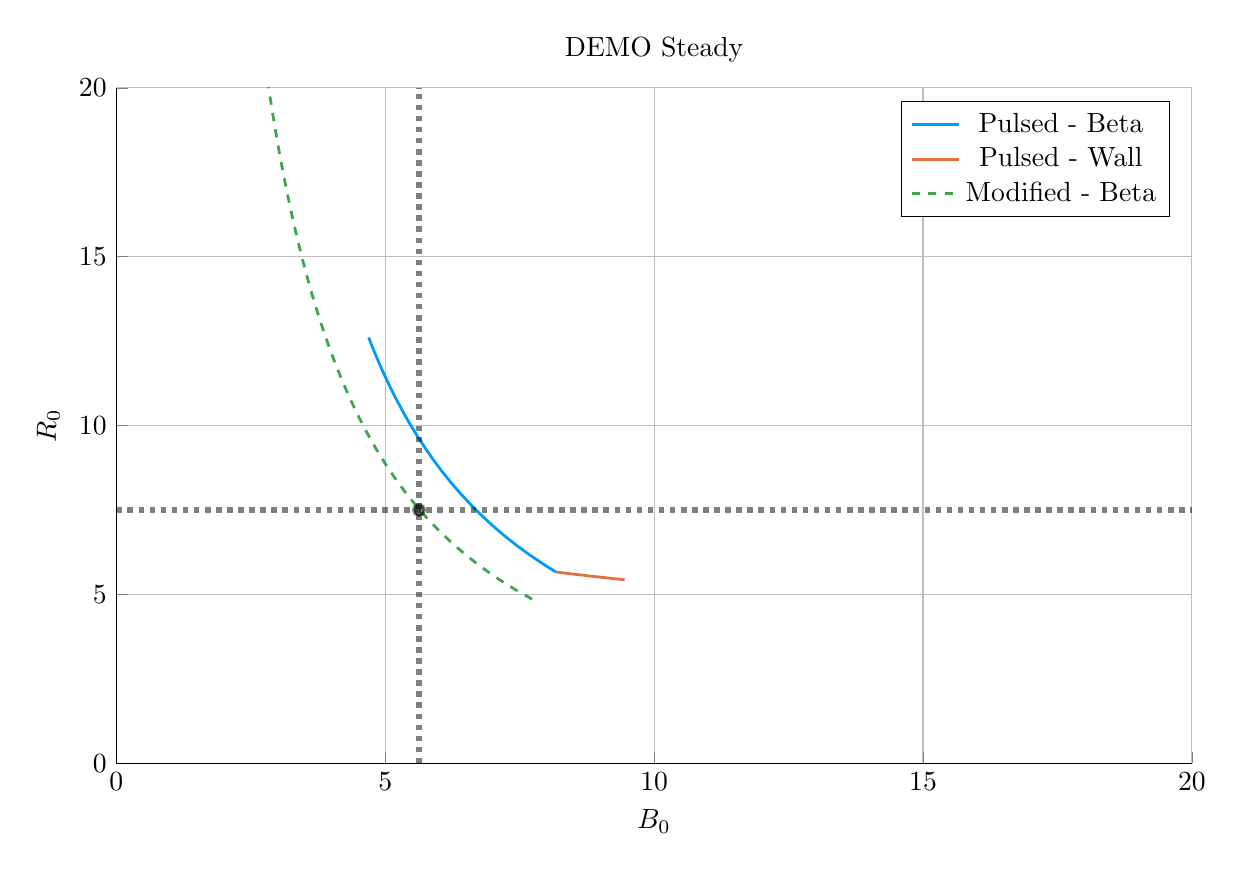
\begin{tikzpicture}[]
\begin{axis}[height = {101.6mm}, ylabel = {${R}_{0}$}, title = {DEMO Steady}, xmin = {0.0}, xmax = {20.0}, ymax = {20.0}, xlabel = {${B}_{0}$}, {unbounded coords=jump, scaled x ticks = false, xticklabel style={rotate = 0}, xmajorgrids = true, xtick = {0.0,5.0,10.0,15.0,20.0}, xticklabels = {0,5,10,15,20}, xtick align = inside, axis lines* = left, scaled y ticks = false, yticklabel style={rotate = 0}, ymajorgrids = true, ytick = {0.0,5.0,10.0,15.0,20.0}, yticklabels = {0,5,10,15,20}, ytick align = inside, axis lines* = left,     xshift = 0.0mm,
    yshift = 0.0mm,
    axis background/.style={fill={rgb,1:red,1.00000000;green,1.00000000;blue,1.00000000}}
, colorbar style={title=}}, ymin = {0.0}, width = {152.4mm}]\addplot+ [color = {rgb,1:red,0.00000000;green,0.60560316;blue,0.97868012},
draw opacity=1.0,
line width=1,
solid,mark = none,
mark size = 2.0,
mark options = {
    color = {rgb,1:red,0.00000000;green,0.00000000;blue,0.00000000}, draw opacity = 1.0,
    fill = {rgb,1:red,0.00000000;green,0.60560316;blue,0.97868012}, fill opacity = 1.0,
    line width = 1,
    rotate = 0,
    solid
}]coordinates {
(8.173486873088942, 5.664794455960266)
(7.942780080136996, 5.894389477908349)
(7.682110747013332, 6.174587309854596)
(7.436076373351653, 6.4617259587740365)
(7.203701032854224, 6.7556817964635885)
(6.984087846006315, 7.056316762210614)
(6.776411507024863, 7.363478485110443)
(6.579911624110169, 7.677000456183209)
(6.393886772782909, 7.996702249919802)
(6.217689175869905, 8.322389794615686)
(6.050719935402341, 8.653855690575247)
(5.892424751644716, 8.990879574996331)
(5.742290072962272, 9.333228532083597)
(5.599839627496144, 9.680657546690735)
(5.464631293842628, 10.03290999955685)
(5.33625427328881, 10.389718201981736)
(5.214326530771975, 10.75080396758328)
(5.098492475718857, 11.115879218594692)
(4.98842085737482, 11.484646623994054)
(4.88380285223036, 11.85680026661456)
(4.784350323760147, 12.232026336259217)
(4.689794236961777, 12.610003845742904)
};
\addlegendentry{Pulsed - Beta}
\addplot+ [color = {rgb,1:red,0.88887350;green,0.43564919;blue,0.27812294},
draw opacity=1.0,
line width=1,
solid,mark = none,
mark size = 2.0,
mark options = {
    color = {rgb,1:red,0.00000000;green,0.00000000;blue,0.00000000}, draw opacity = 1.0,
    fill = {rgb,1:red,0.88887350;green,0.43564919;blue,0.27812294}, fill opacity = 1.0,
    line width = 1,
    rotate = 0,
    solid
}]coordinates {
(9.452194760190558, 5.436039445052516)
(8.82895875946862, 5.541751345019407)
(8.260410483462291, 5.64769543408014)
(8.173486873088942, 5.664794455960266)
};
\addlegendentry{Pulsed - Wall}
\addplot+ [color = {rgb,1:red,0.24222430;green,0.64327509;blue,0.30444865},
draw opacity=1.0,
line width=1,
dashed,mark = none,
mark size = 2.0,
mark options = {
    color = {rgb,1:red,0.00000000;green,0.00000000;blue,0.00000000}, draw opacity = 1.0,
    fill = {rgb,1:red,0.24222430;green,0.64327509;blue,0.30444865}, fill opacity = 1.0,
    line width = 1,
    rotate = 0,
    solid
}]coordinates {
(7.729015258613306, 4.861871150043874)
(7.398090906424027, 5.162615732748398)
(7.087604971989989, 5.475689582149146)
(6.796029845186129, 5.801261884855786)
(6.5219747916377235, 6.139486028413868)
(6.264171517105504, 6.490498735804173)
(6.021461495247516, 6.854419238072999)
(5.792784817023639, 7.231348485954994)
(5.57717035299729, 7.621368405021026)
(5.3737270519036775, 8.024541198865679)
(5.1816362256187425, 8.440908704652248)
(5.000144692923053, 8.870491805097014)
(4.828558673035444, 9.313289900712723)
(4.666238335465348, 9.769280445839089)
(4.512592925835539, 10.23841855166636)
(4.367076398389423, 10.720636659108127)
(4.229183495269078, 11.215844284001262)
(4.098446220614958, 11.723927836706606)
(3.974430664327246, 12.244750517759236)
(3.856734136133517, 12.778152290770123)
(3.744982575583214, 13.323949933321568)
(3.6388282078672565, 13.881937166125676)
(3.537947419047361, 14.45188486023713)
(3.4420388274654035, 15.033541321628862)
(3.3508215308612357, 15.626632651963563)
(3.2640335111230074, 16.230863183919308)
(3.18143018067718, 16.84591598897328)
(3.1027830563428513, 17.471453455103656)
(3.0278785480626333, 18.107117931452404)
(2.956516851312625, 18.752532436599008)
(2.888510933213844, 19.407301426734122)
(2.823685603439882, 20.071011619694055)
(2.761876661959762, 20.74323287052923)
(2.702930116488407, 21.423519094029906)
(2.646701463253573, 22.111409229427537)
(2.593055025340143, 22.806428242329144)
};
\addlegendentry{Modified - Beta}
\addplot+ [color = {rgb,1:red,0.00000000;green,0.00000000;blue,0.00000000},
draw opacity=0.5,
line width=2,
dotted,mark = none,
mark size = 2.0,
mark options = {
    color = {rgb,1:red,0.00000000;green,0.00000000;blue,0.00000000}, draw opacity = 0.5,
    fill = {rgb,1:red,0.00000000;green,0.00000000;blue,0.00000000}, fill opacity = 0.5,
    line width = 1,
    rotate = 0,
    solid
},forget plot]coordinates {
(0.0, 7.5)
(20.0, 7.5)
};
\addplot+ [color = {rgb,1:red,0.00000000;green,0.00000000;blue,0.00000000},
draw opacity=0.5,
line width=2,
dotted,mark = none,
mark size = 2.0,
mark options = {
    color = {rgb,1:red,0.00000000;green,0.00000000;blue,0.00000000}, draw opacity = 0.5,
    fill = {rgb,1:red,0.00000000;green,0.00000000;blue,0.00000000}, fill opacity = 0.5,
    line width = 1,
    rotate = 0,
    solid
},forget plot]coordinates {
(5.627, 0.0)
(5.627, 20.0)
};
\addplot+[draw=none, color = {rgb,1:red,0.00000000;green,0.00000000;blue,0.00000000},
draw opacity=0.5,
line width=0,
solid,mark = *,
mark size = 2.0,
mark options = {
    color = {rgb,1:red,0.00000000;green,0.00000000;blue,0.00000000}, draw opacity = 0.5,
    fill = {rgb,1:red,0.00000000;green,0.00000000;blue,0.00000000}, fill opacity = 0.5,
    line width = 1,
    rotate = 0,
    solid
},forget plot] coordinates {
(5.627, 7.5)
};
\end{axis}

\end{tikzpicture}

    \end{adjustbox}
        \caption{$R_0$ vs $B_0$}
    \end{subfigure}
    \hfill
    \begin{subfigure}[t]{0.45\textwidth}
        \centering
    \begin{adjustbox}{width=\textwidth}
      \Large
      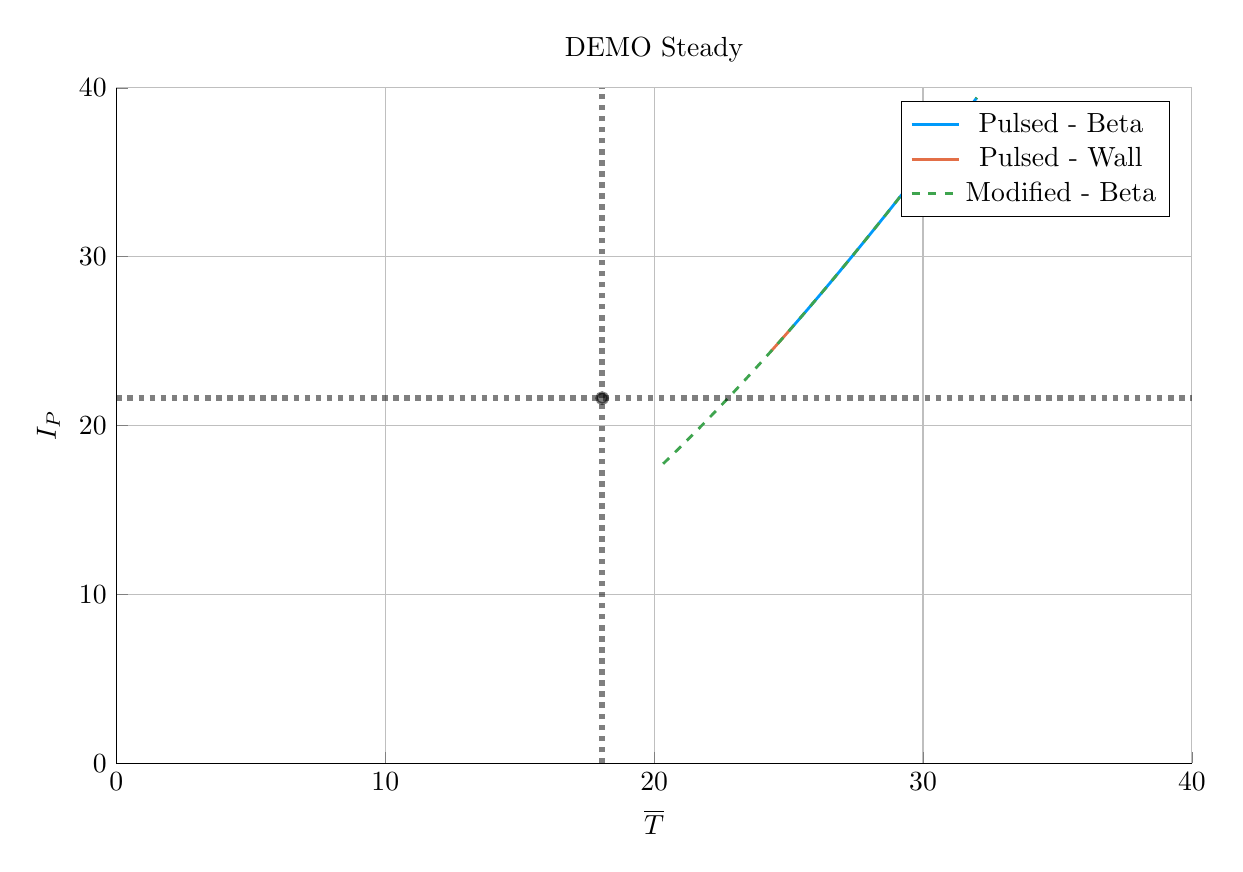
\begin{tikzpicture}[]
\begin{axis}[height = {101.6mm}, ylabel = {${I}_{P}$}, title = {DEMO Steady}, xmin = {0.0}, xmax = {40.0}, ymax = {40.0}, xlabel = {$\overline {T}$}, {unbounded coords=jump, scaled x ticks = false, xticklabel style={rotate = 0}, xmajorgrids = true, xtick = {0.0,10.0,20.0,30.0,40.0}, xticklabels = {0,10,20,30,40}, xtick align = inside, axis lines* = left, scaled y ticks = false, yticklabel style={rotate = 0}, ymajorgrids = true, ytick = {0.0,10.0,20.0,30.0,40.0}, yticklabels = {0,10,20,30,40}, ytick align = inside, axis lines* = left,     xshift = 0.0mm,
    yshift = 0.0mm,
    axis background/.style={fill={rgb,1:red,1.00000000;green,1.00000000;blue,1.00000000}}
, colorbar style={title=}}, ymin = {0.0}, width = {152.4mm}]\addplot+ [color = {rgb,1:red,0.00000000;green,0.60560316;blue,0.97868012},
draw opacity=1.0,
line width=1,
solid,mark = none,
mark size = 2.0,
mark options = {
    color = {rgb,1:red,0.00000000;green,0.00000000;blue,0.00000000}, draw opacity = 1.0,
    fill = {rgb,1:red,0.00000000;green,0.60560316;blue,0.97868012}, fill opacity = 1.0,
    line width = 1,
    rotate = 0,
    solid
}]coordinates {
(25.053735982163357, 25.677558860299992)
(25.333333333333332, 26.189593064380034)
(25.666666666666668, 26.80548085953921)
(26.0, 27.427148406840605)
(26.333333333333332, 28.054440831282633)
(26.666666666666668, 28.68719962041386)
(27.0, 29.325262818659787)
(27.333333333333332, 29.968465226287904)
(27.666666666666668, 30.6166386025962)
(28.0, 31.269611872884024)
(28.333333333333332, 31.92721133872904)
(28.666666666666668, 32.589260891064264)
(29.0, 33.25558222552837)
(29.333333333333332, 33.925995059549685)
(29.666666666666668, 34.60031735061725)
(30.0, 35.27836551518855)
(30.333333333333332, 35.95995464768734)
(30.666666666666668, 36.644898739049395)
(31.0, 37.333010894283476)
(31.333333333333332, 38.02410354852819)
(31.666666666666668, 38.717988681099214)
(32.0, 39.41447802704077)
};
\addlegendentry{Pulsed - Beta}
\addplot+ [color = {rgb,1:red,0.88887350;green,0.43564919;blue,0.27812294},
draw opacity=1.0,
line width=1,
solid,mark = none,
mark size = 2.0,
mark options = {
    color = {rgb,1:red,0.00000000;green,0.00000000;blue,0.00000000}, draw opacity = 1.0,
    fill = {rgb,1:red,0.88887350;green,0.43564919;blue,0.27812294}, fill opacity = 1.0,
    line width = 1,
    rotate = 0,
    solid
}]coordinates {
(24.333333333333332, 24.378107374495485)
(24.666666666666668, 24.975762903314084)
(25.0, 25.579637086786484)
(25.053735982163357, 25.677558860299992)
};
\addlegendentry{Pulsed - Wall}
\addplot+ [color = {rgb,1:red,0.24222430;green,0.64327509;blue,0.30444865},
draw opacity=1.0,
line width=1,
dashed,mark = none,
mark size = 2.0,
mark options = {
    color = {rgb,1:red,0.00000000;green,0.00000000;blue,0.00000000}, draw opacity = 1.0,
    fill = {rgb,1:red,0.24222430;green,0.64327509;blue,0.30444865}, fill opacity = 1.0,
    line width = 1,
    rotate = 0,
    solid
}]coordinates {
(20.333333333333332, 17.737142606162497)
(20.666666666666668, 18.250736761644205)
(21.0, 18.771889258341997)
(21.333333333333332, 19.300518519223587)
(21.666666666666668, 19.836537357082282)
(22.0, 20.37985305559639)
(22.333333333333332, 20.930367463801495)
(22.666666666666668, 21.487977099646507)
(23.0, 22.05257326267931)
(23.333333333333332, 22.62404215595106)
(23.666666666666668, 23.202265017123075)
(24.0, 23.787118258664318)
(24.333333333333332, 24.378473616949)
(24.666666666666668, 24.976198309995638)
(25.0, 25.58015520352756)
(25.333333333333332, 26.19020298497985)
(25.666666666666668, 26.806196345025047)
(26.0, 27.427986166140983)
(26.333333333333332, 28.055419717698932)
(26.666666666666668, 28.688340857006587)
(27.0, 29.3265902357016)
(27.333333333333332, 29.970005510854897)
(27.666666666666668, 30.61842156011136)
(28.0, 31.27167070016686)
(28.333333333333332, 31.92958290785876)
(28.666666666666668, 32.591986043126525)
(29.0, 33.25870607308836)
(29.333333333333332, 33.929567296470175)
(29.666666666666668, 34.604392567622554)
(30.0, 35.28300351936469)
(30.333333333333332, 35.96522078390488)
(30.666666666666668, 36.650864211102025)
(31.0, 37.3397530833557)
(31.333333333333332, 38.03170632643894)
(31.666666666666668, 38.726542715621264)
(32.0, 39.424081076468326)
};
\addlegendentry{Modified - Beta}
\addplot+ [color = {rgb,1:red,0.00000000;green,0.00000000;blue,0.00000000},
draw opacity=0.5,
line width=2,
dotted,mark = none,
mark size = 2.0,
mark options = {
    color = {rgb,1:red,0.00000000;green,0.00000000;blue,0.00000000}, draw opacity = 0.5,
    fill = {rgb,1:red,0.00000000;green,0.00000000;blue,0.00000000}, fill opacity = 0.5,
    line width = 1,
    rotate = 0,
    solid
},forget plot]coordinates {
(0.0, 21.627)
(40.0, 21.627)
};
\addplot+ [color = {rgb,1:red,0.00000000;green,0.00000000;blue,0.00000000},
draw opacity=0.5,
line width=2,
dotted,mark = none,
mark size = 2.0,
mark options = {
    color = {rgb,1:red,0.00000000;green,0.00000000;blue,0.00000000}, draw opacity = 0.5,
    fill = {rgb,1:red,0.00000000;green,0.00000000;blue,0.00000000}, fill opacity = 0.5,
    line width = 1,
    rotate = 0,
    solid
},forget plot]coordinates {
(18.067, 0.0)
(18.067, 40.0)
};
\addplot+[draw=none, color = {rgb,1:red,0.00000000;green,0.00000000;blue,0.00000000},
draw opacity=0.5,
line width=0,
solid,mark = *,
mark size = 2.0,
mark options = {
    color = {rgb,1:red,0.00000000;green,0.00000000;blue,0.00000000}, draw opacity = 0.5,
    fill = {rgb,1:red,0.00000000;green,0.00000000;blue,0.00000000}, fill opacity = 0.5,
    line width = 1,
    rotate = 0,
    solid
},forget plot] coordinates {
(18.067, 21.627)
};
\end{axis}

\end{tikzpicture}

    \end{adjustbox}
        \caption{$I_P$ vs $\overline T$}
    \end{subfigure}
    \hfill \hfill ~\\ ~\\ ~\\
    \caption{Demo Steady Model Comparison} ~\\
\end{figure*}

\begin{table}[h!]
\centering  
\caption{Demo Steady Variables}
\hfill
\begin{subtable}[t]{0.4\textwidth}
\centering  
\caption{Input Variables} ~\\
\begin{tabular}{ c|c } 

Input            & Value           \\
\hline
$H$              & 1.4             \\
$Q$              & 24.46           \\
$N_{G}$          & 1.2             \\
$\epsilon$       & 0.385           \\
$\kappa_{95}$    & 1.8             \\
$\delta_{95}$    & 0.333           \\
$\nu_{n}$        & 0.3972          \\
$\nu_{T}$        & 0.9187          \\
$l_{i}$          & 0.9             \\
$A$              & 2.856           \\
$Z_{eff}$        & 4.708           \\
$f_{D}$          & 0.7366          \\
$\tau_{FT}$      & 1.6e9           \\
$B_{CS}$         & 12.85           \\

\end{tabular}
\end{subtable}
\hfill
\begin{subtable}[t]{0.5\textwidth}
\centering  
\caption{Output Variables} ~\\
\begin{tabular}{ c|c|c } 

Output           & Original         & Fussy.jl        \\  
\hline
$R_{0}$          & 7.5              & 8.2           \\
$B_{0}$          & 5.627            & 6.307           \\
$I_{P}$          & 21.63            & 30.93           \\
$\overline n$    & 0.8746           & 1.048           \\
$\overline T$    & 18.07            & 27.83           \\
$\beta_{N}$       & 0.038            & -           \\
$q_{95}$         & 4.405            & 3.761           \\
$P_{W}$          & 1.911            & 4.151           \\
$f_{BS}$         & 0.611            & 0.424          \\
$f_{CD}$         & 0.389            & 0.576          \\
$f_{IN}$         & -              & -             \\
$\volume$         & 2217           & 2879          \\
$P_{F}$          & 3255           & 8971          \\
$\eta_{CD}$      & 0.4152           & -          \\

\end{tabular}
\end{subtable}
\hfill
\hfill
\end{table}

\newpage 

\subsubsection{DEMO Pulsed -- A Pulsed ITER Successor}

This pulsed version of DEMO is the only reactor in our collection that is not run in steady-state. As such, it may be the most important one. The first thing that is abundantly clear is that this design actually has no valid wall loading portion -- only a kink and beta curve exist! Even so, the results match pretty well. It should be noted, though, that this current drive is treated as an input and not solved self-consistently.

\begin{figure*}[h!]
    \centering
    \hfill 
    \begin{subfigure}[t]{0.45\textwidth}
        \centering
    \begin{adjustbox}{width=\textwidth}
      \Large
      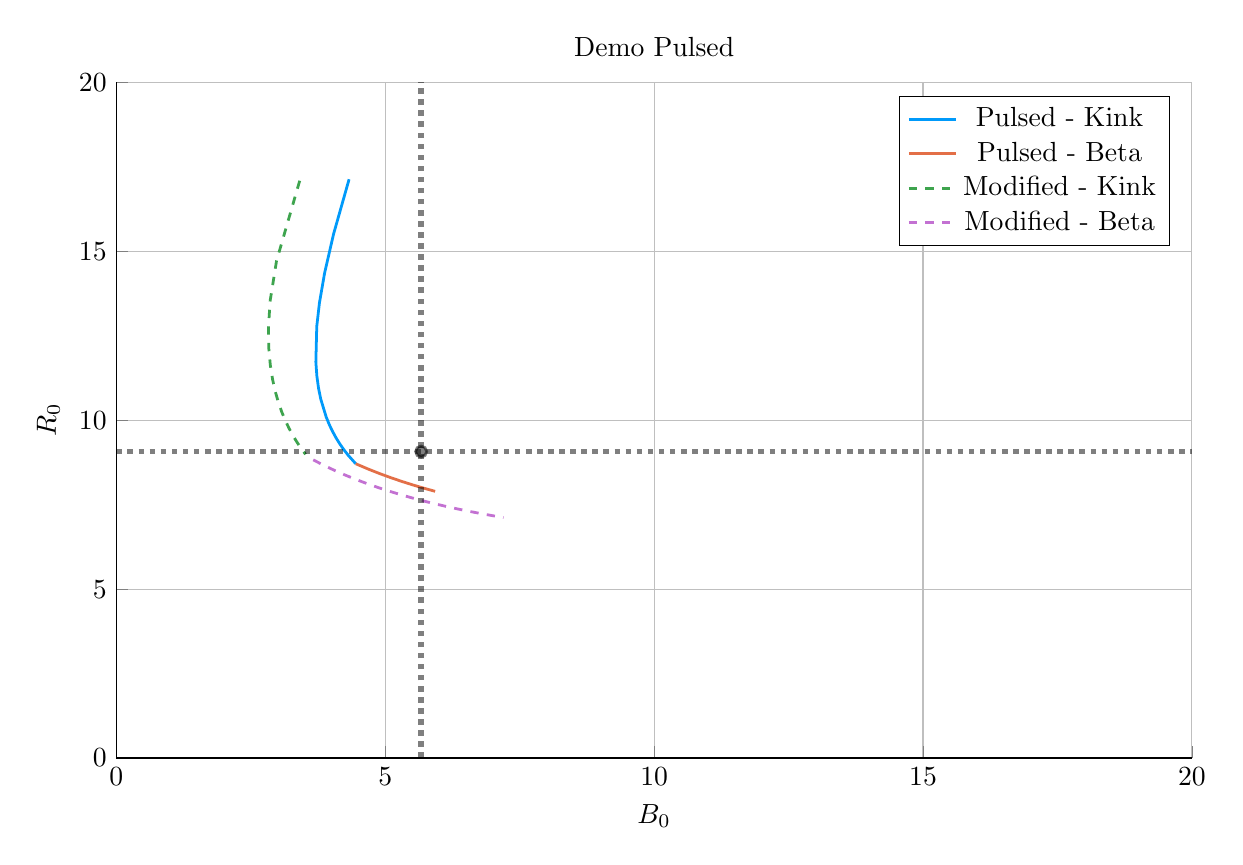
\begin{tikzpicture}[]
\begin{axis}[height = {101.6mm}, ylabel = {${R}_{0}$}, title = {Demo Pulsed}, xmin = {0.0}, xmax = {20.0}, ymax = {20.0}, xlabel = {${B}_{0}$}, {unbounded coords=jump, scaled x ticks = false, xticklabel style={rotate = 0}, xmajorgrids = true, xtick = {0.0,5.0,10.0,15.0,20.0}, xticklabels = {0,5,10,15,20}, xtick align = inside, axis lines* = left, scaled y ticks = false, yticklabel style={rotate = 0}, ymajorgrids = true, ytick = {0.0,5.0,10.0,15.0,20.0}, yticklabels = {0,5,10,15,20}, ytick align = inside, axis lines* = left,     xshift = 0.0mm,
    yshift = 0.0mm,
    axis background/.style={fill={rgb,1:red,1.00000000;green,1.00000000;blue,1.00000000}}
, colorbar style={title=}}, ymin = {0.0}, width = {152.4mm}]\addplot+ [color = {rgb,1:red,0.00000000;green,0.60560316;blue,0.97868012},
draw opacity=1.0,
line width=1,
solid,mark = none,
mark size = 2.0,
mark options = {
    color = {rgb,1:red,0.00000000;green,0.00000000;blue,0.00000000}, draw opacity = 1.0,
    fill = {rgb,1:red,0.00000000;green,0.60560316;blue,0.97868012}, fill opacity = 1.0,
    line width = 1,
    rotate = 0,
    solid
}]coordinates {
(4.327031075670194, 17.134796748649162)
(4.038214026054326, 15.511755022601415)
(3.8713719163129245, 14.355562963913712)
(3.7758613845615545, 13.476675762289453)
(3.7257856761317214, 12.778294295391971)
(3.7090473695925437, 11.723065749829066)
(3.727711597554826, 11.30970201784727)
(3.7586131667481433, 10.94971275897184)
(3.799052518631718, 10.632190690377048)
(3.901290136389271, 10.09455415135144)
(3.960577465316514, 9.863813619410237)
(4.0241209645210345, 9.653307397969705)
(4.0912717805663785, 9.460162902699798)
(4.161514602943343, 9.28206292757184)
(4.2344343960723005, 9.117114543572253)
(4.309692554546368, 8.963753917462126)
(4.450417240491067, 8.712493965092264)
};
\addlegendentry{Pulsed - Kink}
\addplot+ [color = {rgb,1:red,0.88887350;green,0.43564919;blue,0.27812294},
draw opacity=1.0,
line width=1,
solid,mark = none,
mark size = 2.0,
mark options = {
    color = {rgb,1:red,0.00000000;green,0.00000000;blue,0.00000000}, draw opacity = 1.0,
    fill = {rgb,1:red,0.88887350;green,0.43564919;blue,0.27812294}, fill opacity = 1.0,
    line width = 1,
    rotate = 0,
    solid
}]coordinates {
(4.450417240491067, 8.712493965092264)
(4.490148631384312, 8.684308742646298)
(4.692490181445514, 8.547262773806349)
(4.8960344619053355, 8.41947837460442)
(5.100651132702229, 8.30014929484307)
(5.306202822090688, 8.188581738801314)
(5.512545696627038, 8.084175191078112)
(5.719530043226767, 7.986407002697611)
(5.927000883375481, 7.894819882619234)
};
\addlegendentry{Pulsed - Beta}
\addplot+ [color = {rgb,1:red,0.24222430;green,0.64327509;blue,0.30444865},
draw opacity=1.0,
line width=1,
dashed,mark = none,
mark size = 2.0,
mark options = {
    color = {rgb,1:red,0.00000000;green,0.00000000;blue,0.00000000}, draw opacity = 1.0,
    fill = {rgb,1:red,0.24222430;green,0.64327509;blue,0.30444865}, fill opacity = 1.0,
    line width = 1,
    rotate = 0,
    solid
}]coordinates {
(3.4087424183072135, 17.090884129081292)
(2.977074181068944, 14.713048632784332)
(2.8592500074202523, 13.541171522519205)
(2.827199220063259, 12.740024138753894)
(2.8339789008667826, 12.12574468151967)
(2.862412302880871, 11.626187613249266)
(2.9044598258085443, 11.205091848948229)
(2.95577893007882, 10.841432203317366)
(3.0137895352525907, 10.521822649209419)
(3.076849710218805, 10.23716073884787)
(3.1438583711612704, 9.980947801083442)
(3.214045733980633, 9.748367275345563)
(3.2868548955983727, 9.535742205343247)
(3.361871149981842, 9.340197658526863)
(3.4387778750377818, 9.15944098345979)
(3.5173279629378453, 8.991613349767409)
};
\addlegendentry{Modified - Kink}
\addplot+ [color = {rgb,1:red,0.76444018;green,0.44411178;blue,0.82429754},
draw opacity=1.0,
line width=1,
dashed,mark = none,
mark size = 2.0,
mark options = {
    color = {rgb,1:red,0.00000000;green,0.00000000;blue,0.00000000}, draw opacity = 1.0,
    fill = {rgb,1:red,0.76444018;green,0.44411178;blue,0.82429754}, fill opacity = 1.0,
    line width = 1,
    rotate = 0,
    solid
}]coordinates {
(3.6607028750648505, 8.825949645171955)
(3.8574448036470477, 8.664618827122876)
(4.056375867871351, 8.51434867582932)
(4.257366397480293, 8.374075613831488)
(4.460279103534801, 8.242896218794312)
(4.664969389370631, 8.12003771613466)
(4.871285596007394, 8.004834914067093)
(5.07906923307514, 7.896711937521184)
(5.288155233306219, 7.795167587687744)
(5.498372259673351, 7.699763475973523)
(5.709543087166185, 7.610114306522102)
(5.921485076209294, 7.525879840414137)
(6.134010749367255, 7.446758190646709)
(6.346928478632384, 7.372480180910637)
(6.560043285872518, 7.302804563889649)
(6.773157754368795, 7.237513941672651)
(6.986073044284746, 7.176411266758267)
(7.198590001107076, 7.119316828230052)
};
\addlegendentry{Modified - Beta}
\addplot+ [color = {rgb,1:red,0.00000000;green,0.00000000;blue,0.00000000},
draw opacity=0.5,
line width=2,
dotted,mark = none,
mark size = 2.0,
mark options = {
    color = {rgb,1:red,0.00000000;green,0.00000000;blue,0.00000000}, draw opacity = 0.5,
    fill = {rgb,1:red,0.00000000;green,0.00000000;blue,0.00000000}, fill opacity = 0.5,
    line width = 1,
    rotate = 0,
    solid
},forget plot]coordinates {
(0.0, 9.072)
(20.0, 9.072)
};
\addplot+ [color = {rgb,1:red,0.00000000;green,0.00000000;blue,0.00000000},
draw opacity=0.5,
line width=2,
dotted,mark = none,
mark size = 2.0,
mark options = {
    color = {rgb,1:red,0.00000000;green,0.00000000;blue,0.00000000}, draw opacity = 0.5,
    fill = {rgb,1:red,0.00000000;green,0.00000000;blue,0.00000000}, fill opacity = 0.5,
    line width = 1,
    rotate = 0,
    solid
},forget plot]coordinates {
(5.667, 0.0)
(5.667, 20.0)
};
\addplot+[draw=none, color = {rgb,1:red,0.00000000;green,0.00000000;blue,0.00000000},
draw opacity=0.5,
line width=0,
solid,mark = *,
mark size = 2.0,
mark options = {
    color = {rgb,1:red,0.00000000;green,0.00000000;blue,0.00000000}, draw opacity = 0.5,
    fill = {rgb,1:red,0.00000000;green,0.00000000;blue,0.00000000}, fill opacity = 0.5,
    line width = 1,
    rotate = 0,
    solid
},forget plot] coordinates {
(5.667, 9.072)
};
\end{axis}

\end{tikzpicture}

    \end{adjustbox}
        \caption{$R_0$ vs $B_0$}
    \end{subfigure}
    \hfill
    \begin{subfigure}[t]{0.45\textwidth}
        \centering
    \begin{adjustbox}{width=\textwidth}
      \Large
      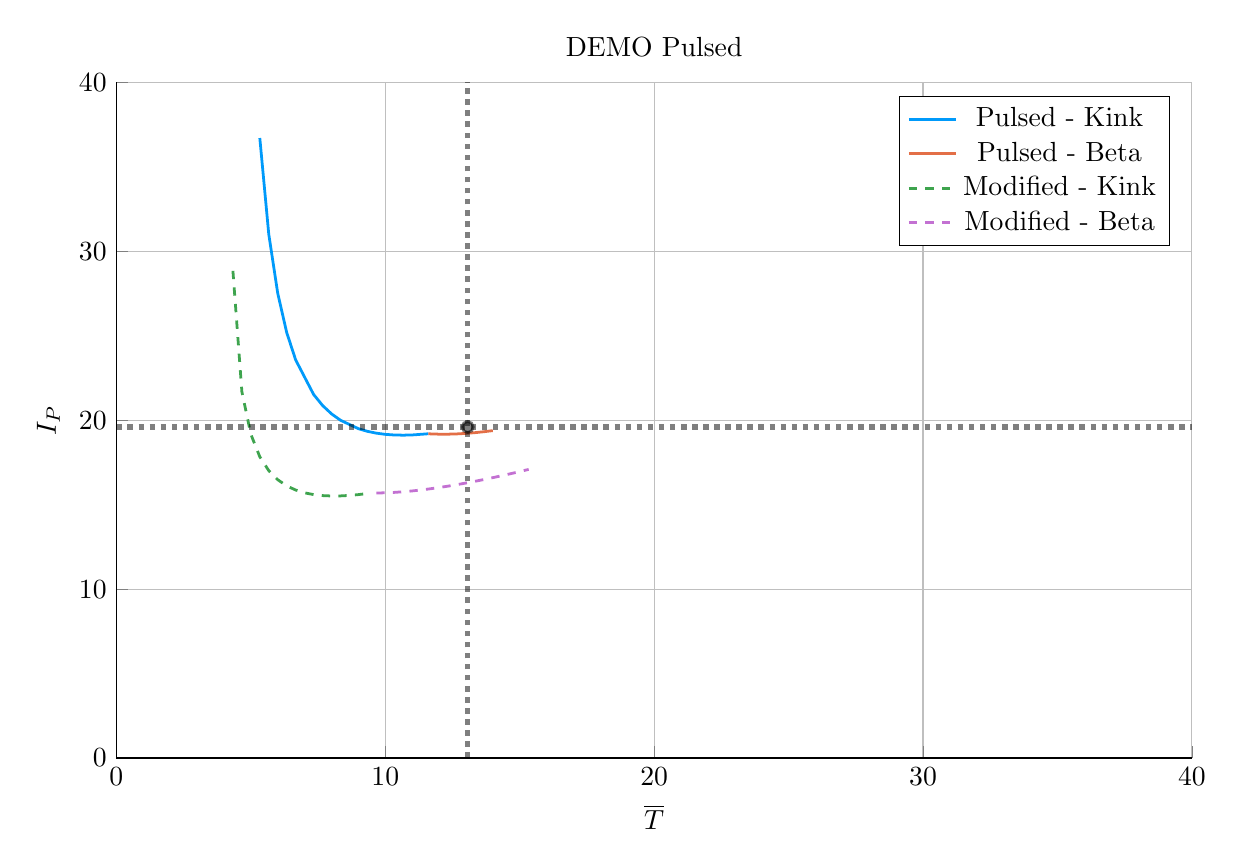
\begin{tikzpicture}[]
\begin{axis}[height = {101.6mm}, ylabel = {${I}_{P}$}, title = {DEMO Pulsed}, xmin = {0.0}, xmax = {40.0}, ymax = {40.0}, xlabel = {$\overline {T}$}, {unbounded coords=jump, scaled x ticks = false, xticklabel style={rotate = 0}, xmajorgrids = true, xtick = {0.0,10.0,20.0,30.0,40.0}, xticklabels = {0,10,20,30,40}, xtick align = inside, axis lines* = left, scaled y ticks = false, yticklabel style={rotate = 0}, ymajorgrids = true, ytick = {0.0,10.0,20.0,30.0,40.0}, yticklabels = {0,10,20,30,40}, ytick align = inside, axis lines* = left,     xshift = 0.0mm,
    yshift = 0.0mm,
    axis background/.style={fill={rgb,1:red,1.00000000;green,1.00000000;blue,1.00000000}}
, colorbar style={title=}}, ymin = {0.0}, width = {152.4mm}]\addplot+ [color = {rgb,1:red,0.00000000;green,0.60560316;blue,0.97868012},
draw opacity=1.0,
line width=1,
solid,mark = none,
mark size = 2.0,
mark options = {
    color = {rgb,1:red,0.00000000;green,0.00000000;blue,0.00000000}, draw opacity = 1.0,
    fill = {rgb,1:red,0.00000000;green,0.60560316;blue,0.97868012}, fill opacity = 1.0,
    line width = 1,
    rotate = 0,
    solid
}]coordinates {
(5.333333333333333, 36.71051032912112)
(5.666666666666667, 31.014995367356207)
(6.0, 27.51734786322149)
(6.333333333333333, 25.19534286389616)
(6.666666666666667, 23.57285610926683)
(7.333333333333333, 21.52905816503197)
(7.666666666666667, 20.874444053021588)
(8.0, 20.377542510464334)
(8.333333333333334, 19.99951688957442)
(9.0, 19.499202175706746)
(9.333333333333334, 19.343044014643887)
(9.666666666666666, 19.233955791269285)
(10.0, 19.16365729524907)
(10.333333333333334, 19.125701869840853)
(10.666666666666666, 19.11499858904485)
(11.0, 19.127475979338943)
(11.600962879632572, 19.198383823705257)
};
\addlegendentry{Pulsed - Kink}
\addplot+ [color = {rgb,1:red,0.88887350;green,0.43564919;blue,0.27812294},
draw opacity=1.0,
line width=1,
solid,mark = none,
mark size = 2.0,
mark options = {
    color = {rgb,1:red,0.00000000;green,0.00000000;blue,0.00000000}, draw opacity = 1.0,
    fill = {rgb,1:red,0.88887350;green,0.43564919;blue,0.27812294}, fill opacity = 1.0,
    line width = 1,
    rotate = 0,
    solid
}]coordinates {
(11.600962879632572, 19.198383823705257)
(11.666666666666666, 19.192414153878335)
(12.0, 19.174087186739918)
(12.333333333333334, 19.17397121853779)
(12.666666666666666, 19.189978018951553)
(13.0, 19.220357277326283)
(13.333333333333334, 19.263633100211838)
(13.666666666666666, 19.31855421750887)
(14.0, 19.384054548489104)
};
\addlegendentry{Pulsed - Beta}
\addplot+ [color = {rgb,1:red,0.24222430;green,0.64327509;blue,0.30444865},
draw opacity=1.0,
line width=1,
dashed,mark = none,
mark size = 2.0,
mark options = {
    color = {rgb,1:red,0.00000000;green,0.00000000;blue,0.00000000}, draw opacity = 1.0,
    fill = {rgb,1:red,0.24222430;green,0.64327509;blue,0.30444865}, fill opacity = 1.0,
    line width = 1,
    rotate = 0,
    solid
}]coordinates {
(4.333333333333333, 28.845639077165217)
(4.666666666666667, 21.687713986294685)
(5.0, 19.170340224057398)
(5.333333333333333, 17.83397336320386)
(5.666666666666667, 17.01478565989059)
(6.0, 16.477486603636205)
(6.333333333333333, 16.113958654578386)
(6.666666666666667, 15.866460603971907)
(7.0, 15.700928946757587)
(7.333333333333333, 15.59578560596909)
(7.666666666666667, 15.536607983152381)
(8.0, 15.513342675582972)
(8.333333333333334, 15.518740955012225)
(8.666666666666666, 15.547428978968492)
(9.0, 15.595329068459918)
(9.333333333333334, 15.659285368310089)
};
\addlegendentry{Modified - Kink}
\addplot+ [color = {rgb,1:red,0.76444018;green,0.44411178;blue,0.82429754},
draw opacity=1.0,
line width=1,
dashed,mark = none,
mark size = 2.0,
mark options = {
    color = {rgb,1:red,0.00000000;green,0.00000000;blue,0.00000000}, draw opacity = 1.0,
    fill = {rgb,1:red,0.76444018;green,0.44411178;blue,0.82429754}, fill opacity = 1.0,
    line width = 1,
    rotate = 0,
    solid
}]coordinates {
(9.666666666666666, 15.691192911261952)
(10.0, 15.70165788278533)
(10.333333333333334, 15.726578234093749)
(10.666666666666666, 15.764127054896537)
(11.0, 15.812802650736373)
(11.333333333333334, 15.871360766004056)
(11.666666666666666, 15.938763317563621)
(12.0, 16.014139065408)
(12.333333333333334, 16.09675304572932)
(12.666666666666666, 16.185982524147033)
(13.0, 16.281297862810217)
(13.333333333333334, 16.382247130746602)
(13.666666666666666, 16.488443597982137)
(14.0, 16.5995554722192)
(14.333333333333334, 16.715297396529092)
(14.666666666666666, 16.83542334285969)
(15.0, 16.959720624053933)
(15.333333333333334, 17.088004807739882)
};
\addlegendentry{Modified - Beta}
\addplot+ [color = {rgb,1:red,0.00000000;green,0.00000000;blue,0.00000000},
draw opacity=0.5,
line width=2,
dotted,mark = none,
mark size = 2.0,
mark options = {
    color = {rgb,1:red,0.00000000;green,0.00000000;blue,0.00000000}, draw opacity = 0.5,
    fill = {rgb,1:red,0.00000000;green,0.00000000;blue,0.00000000}, fill opacity = 0.5,
    line width = 1,
    rotate = 0,
    solid
},forget plot]coordinates {
(0.0, 19.6)
(40.0, 19.6)
};
\addplot+ [color = {rgb,1:red,0.00000000;green,0.00000000;blue,0.00000000},
draw opacity=0.5,
line width=2,
dotted,mark = none,
mark size = 2.0,
mark options = {
    color = {rgb,1:red,0.00000000;green,0.00000000;blue,0.00000000}, draw opacity = 0.5,
    fill = {rgb,1:red,0.00000000;green,0.00000000;blue,0.00000000}, fill opacity = 0.5,
    line width = 1,
    rotate = 0,
    solid
},forget plot]coordinates {
(13.065, 0.0)
(13.065, 40.0)
};
\addplot+[draw=none, color = {rgb,1:red,0.00000000;green,0.00000000;blue,0.00000000},
draw opacity=0.5,
line width=0,
solid,mark = *,
mark size = 2.0,
mark options = {
    color = {rgb,1:red,0.00000000;green,0.00000000;blue,0.00000000}, draw opacity = 0.5,
    fill = {rgb,1:red,0.00000000;green,0.00000000;blue,0.00000000}, fill opacity = 0.5,
    line width = 1,
    rotate = 0,
    solid
},forget plot] coordinates {
(13.065, 19.6)
};
\end{axis}

\end{tikzpicture}

    \end{adjustbox}
        \caption{$I_P$ vs $\overline T$}
    \end{subfigure}
    \hfill \hfill ~\\ ~\\ ~\\
    \caption{Demo Pulsed Model Comparison} ~\\
\end{figure*}

\begin{table}[h!]
\centering  
\caption{Demo Pulsed Variables}
\hfill
\begin{subtable}[t]{0.4\textwidth}
\centering  
\caption{Input Variables} ~\\
\begin{tabular}{ c|c } 

Input            & Value           \\
\hline
$H$              & 1.1             \\
$Q$              & 39.86           \\
$N_{G}$          & 1.2             \\
$\epsilon$       & 0.3226          \\
$\kappa_{95}$    & 1.59            \\
$\delta_{95}$    & 0.333           \\
$\nu_{n}$        & 0.27            \\
$\nu_{T}$        & 1.094           \\
$l_{i}$          & 1.155           \\
$A$              & 2.735           \\
$Z_{eff}$        & 2.584           \\
$f_{D}$          & 0.7753          \\
$\tau_{FT}$      & 7273          \\
$B_{CS}$         & 12.77           \\

\end{tabular}
\end{subtable}
\hfill
\begin{subtable}[t]{0.5\textwidth}
\centering  
\caption{Output Variables} ~\\
\begin{tabular}{ c|c|c } 

Output           & Original         & Fussy.jl        \\
\hline
$R_{0}$          & 9.07            & 8.10             \\
$B_{0}$          & 5.67            & 5.48            \\
$I_{P}$          & 19.6             & 19.3           \\
$\overline n$    & 0.7983           & 0.9795          \\
$\overline T$    & 13.06            & 13.28           \\
$\beta_{N}$       & 0.0259           & -          \\
$q_{95}$         & 3.247            & 2.853           \\
$P_{W}$          & 1.05             & 1.47           \\
$f_{BS}$         & 0.348            & 0.164          \\
$f_{CD}$         & 0.096            & 0.106          \\
$f_{IN}$         & 0.557            & 0.730          \\
$\volume$         & 2502           & 1751          \\
$P_{F}$          & 2037           & 2376          \\
$\eta_{CD}$      & 0.2721           & -     

\end{tabular}
\end{subtable}
\hfill
\hfill
\end{table}

\section{Developing Prototype Reactors}

Now that the model used in Fussy.jl has been tested against other fusion systems codes in the field, we will develop our own prototype reactors. Because this paper is about making a levelized comparison of pulsed and steady-state tokamaks, we will develop middle-of-the-road reactors that only differ by operating mode. 

The steady-state prototype, Charybdis, is the obvious choice to start with -- as the model was tested against four of these typed reactors. It was also pointed out that the model did remarkably well when recreating ARC. As the authors share many of the ARC team's philosophies, Charybdis uses fixed parameters very similar to them.

Next, although led to believe Charybdis' pulsed twin reactor -- Proteus -- would be created by a simple flip of the switch, it was a slight oversimplification. The first difference is that the pulsed twin, Proteus, is assumed to be purely pulsed: $\eta_{CD} = 0$. Further, the bootstrap current is much less important than it was for steady-state tokamaks. This corresponds to a current profile peaked at the origin -- i.e. a parabola. Numerically, this is done by raising $l_i$ from around 5.5 to 6.

The final difference creates the largest change in the twin reactors: the choice of miracle. As hinted several times before, the H factor is a common way designers artificially boost the confinement of their machines. This H value will thus be the miracle for Charybdis, the steady-state prototype. Next, as the main conclusion of this paper is to state the advantages of high magnetic field, a free way to boost a central solenoid using HTS coils will be employed.

Opposite the order of how they were designed, the goal now is to lock down a value of $B_{CS}$ for Proteus and then use it to set the H factor for Charybdis. This selection algorithm is depicted in \cref{fig:selection}. For Proteus, the point locked down was $B_{CS} = 20 \ \textnormal{T}$, which occurred at a fusion power ($P_F$) of around 1250 MW. As shown in the cost curve, this was at a point where the ratio between the minimum capital cost and the minimum cost-per-watt saturated. This choice of a 1250 MW reactor then led to Charybdis having an H factor of 1.7.

\begin{figure}[h!]
\centering
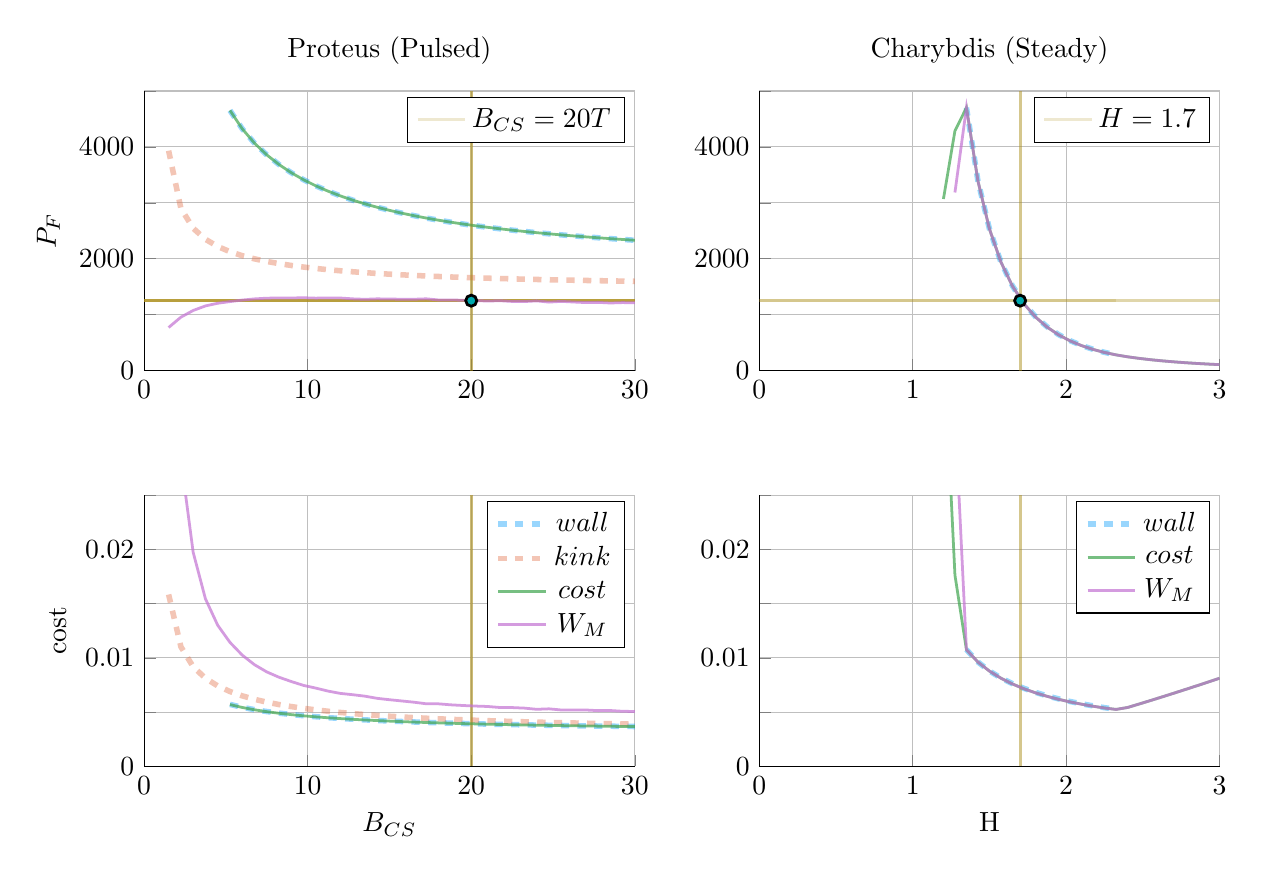
\begin{tikzpicture}[]
\begin{axis}[height = {51.32916666666667mm}, ylabel = {$P_F$}, title = {Proteus (Pulsed)}, xmin = {0}, xmax = {30.0}, ymax = {5000.0}, xlabel = {}, {unbounded coords=jump, scaled x ticks = false, xticklabel style={rotate = 0}, xmajorgrids = true, xtick = {0.0,10.0,20.0,30.0}, xticklabels = {0,10,20,30}, xtick align = inside, axis lines* = left, scaled y ticks = false, yticklabel style={rotate = 0}, ymajorgrids = true, ytick = {0,1000,2000,3000,4000,5000}, yticklabels = {0,,2000,,4000,}, ytick align = inside, axis lines* = left,     xshift = 0.0mm,
    yshift = 50.27mm,
    axis background/.style={fill={rgb,1:red,1.00000000;green,1.00000000;blue,1.00000000}}
}, ymin = {2.220446049250313e-16}, width = {78.14027777777778mm}]\addplot+ [color = {rgb,1:red,0.67554396;green,0.55566233;blue,0.09423434},
draw opacity=0.2,
line width=1,
solid,mark = none,
mark size = 2.0,
mark options = {
    color = {rgb,1:red,0.00000000;green,0.00000000;blue,0.00000000}, draw opacity = 1.0,
    fill = {rgb,1:red,0.67554396;green,0.55566233;blue,0.09423434}, fill opacity = 1.0,
    line width = 1,
    rotate = 0,
    solid
}]coordinates {
(20.0, 2.220446049250313e-16)
(20.0, 5000.0)
};
\addlegendentry{$B_{CS} = 20 T$}
\addplot+ [color = {rgb,1:red,0.67554396;green,0.55566233;blue,0.09423434},
draw opacity=0.2,
line width=1,
solid,mark = none,
mark size = 2.0,
mark options = {
    color = {rgb,1:red,0.00000000;green,0.00000000;blue,0.00000000}, draw opacity = 1.0,
    fill = {rgb,1:red,0.67554396;green,0.55566233;blue,0.09423434}, fill opacity = 1.0,
    line width = 1,
    rotate = 0,
    solid
},forget plot]coordinates {
(0.0, 1250.0)
(30.0, 1250.0)
};
\addplot+[draw=none, color = {rgb,1:red,0.00000048;green,0.66575898;blue,0.68099695},
draw opacity=1.0,
line width=0,
solid,mark = *,
mark size = 2.0,
mark options = {
    color = {rgb,1:red,0.00000000;green,0.00000000;blue,0.00000000}, draw opacity = 1.0,
    fill = {rgb,1:red,0.00000048;green,0.66575898;blue,0.68099695}, fill opacity = 1.0,
    line width = 1,
    rotate = 0,
    solid
},forget plot] coordinates {
(20, 1250)
};
\addplot+ [color = {rgb,1:red,0.67554396;green,0.55566233;blue,0.09423434},
draw opacity=0.2,
line width=1,
solid,mark = none,
mark size = 2.0,
mark options = {
    color = {rgb,1:red,0.00000000;green,0.00000000;blue,0.00000000}, draw opacity = 1.0,
    fill = {rgb,1:red,0.67554396;green,0.55566233;blue,0.09423434}, fill opacity = 1.0,
    line width = 1,
    rotate = 0,
    solid
},forget plot]coordinates {
(0.0, 1250.0)
(30.0, 1250.0)
};
\addplot+ [color = {rgb,1:red,0.00000000;green,0.60560316;blue,0.97868012},
draw opacity=0.4,
line width=2,
dashed,mark = none,
mark size = 2.0,
mark options = {
    color = {rgb,1:red,0.00000000;green,0.00000000;blue,0.00000000}, draw opacity = 1.0,
    fill = {rgb,1:red,0.00000000;green,0.60560316;blue,0.97868012}, fill opacity = 1.0,
    line width = 1,
    rotate = 0,
    solid
},forget plot]coordinates {
(5.25, 4651.734735476011)
(6.0, 4323.6250098364)
(6.75, 4065.99692078527)
(7.5, 3857.273578687972)
(8.25, 3684.1342593418663)
(9.0, 3537.844669896544)
(9.75, 3412.404653539425)
(10.5, 3303.536032694244)
(11.25, 3208.094051273514)
(12.0, 3123.707522754923)
(12.75, 3048.5495054628623)
(13.5, 2981.185980181023)
(14.25, 2920.472987010462)
(15.0, 2865.484885250518)
(15.75, 2815.463186166668)
(16.5, 2769.7793320244814)
(17.25, 2727.9071420752607)
(18.0, 2689.4020933235493)
(18.75, 2653.885520176901)
(19.5, 2621.0324111911764)
(20.25, 2590.561874678777)
(21.0, 2562.2296107375955)
(21.75, 2535.8219099446264)
(22.5, 2511.150826555893)
(23.25, 2488.050264495335)
(24.0, 2466.372779394113)
(24.75, 2445.986947213969)
(25.5, 2426.775184780072)
(26.25, 2408.6319334297787)
(27.0, 2391.4621364565396)
(27.75, 2375.1799557182867)
(28.5, 2359.707684182671)
(29.25, 2344.974819785335)
(30.0, 2330.917272823136)
};
\addplot+ [color = {rgb,1:red,0.67554396;green,0.55566233;blue,0.09423434},
draw opacity=0.2,
line width=1,
solid,mark = none,
mark size = 2.0,
mark options = {
    color = {rgb,1:red,0.00000000;green,0.00000000;blue,0.00000000}, draw opacity = 1.0,
    fill = {rgb,1:red,0.67554396;green,0.55566233;blue,0.09423434}, fill opacity = 1.0,
    line width = 1,
    rotate = 0,
    solid
},forget plot]coordinates {
(20.0, 2.220446049250313e-16)
(20.0, 5000.0)
};
\addplot+ [color = {rgb,1:red,0.67554396;green,0.55566233;blue,0.09423434},
draw opacity=0.2,
line width=1,
solid,mark = none,
mark size = 2.0,
mark options = {
    color = {rgb,1:red,0.00000000;green,0.00000000;blue,0.00000000}, draw opacity = 1.0,
    fill = {rgb,1:red,0.67554396;green,0.55566233;blue,0.09423434}, fill opacity = 1.0,
    line width = 1,
    rotate = 0,
    solid
},forget plot]coordinates {
(0.0, 1250.0)
(30.0, 1250.0)
};
\addplot+ [color = {rgb,1:red,0.67554396;green,0.55566233;blue,0.09423434},
draw opacity=0.2,
line width=1,
solid,mark = none,
mark size = 2.0,
mark options = {
    color = {rgb,1:red,0.00000000;green,0.00000000;blue,0.00000000}, draw opacity = 1.0,
    fill = {rgb,1:red,0.67554396;green,0.55566233;blue,0.09423434}, fill opacity = 1.0,
    line width = 1,
    rotate = 0,
    solid
},forget plot]coordinates {
(0.0, 1250.0)
(30.0, 1250.0)
};
\addplot+ [color = {rgb,1:red,0.88887350;green,0.43564919;blue,0.27812294},
draw opacity=0.4,
line width=2,
dashed,mark = none,
mark size = 2.0,
mark options = {
    color = {rgb,1:red,0.00000000;green,0.00000000;blue,0.00000000}, draw opacity = 1.0,
    fill = {rgb,1:red,0.88887350;green,0.43564919;blue,0.27812294}, fill opacity = 1.0,
    line width = 1,
    rotate = 0,
    solid
},forget plot]coordinates {
(1.5, 3931.6170696070676)
(2.25, 2900.7235747979908)
(3.0, 2544.8446560898715)
(3.75, 2348.228116500571)
(4.5, 2219.0134794713767)
(5.25, 2125.815532966674)
(6.0, 2054.566085735622)
(6.75, 1997.8824990557177)
(7.5, 1951.4633680592258)
(8.25, 1912.6074536455505)
(9.0, 1879.5196356674505)
(9.75, 1850.953068441656)
(10.5, 1826.0101459658863)
(11.25, 1804.02551415983)
(12.0, 1784.493638745381)
(12.75, 1767.0222758941622)
(13.5, 1751.3015387280175)
(14.25, 1737.0827328069474)
(15.0, 1724.1634044428295)
(15.75, 1712.376890482151)
(16.5, 1701.5841921715175)
(17.25, 1691.6685698179294)
(18.0, 1682.530881991843)
(18.75, 1674.0861755860074)
(19.5, 1666.2615100001372)
(20.25, 1658.9932835127363)
(21.0, 1652.2262595201232)
(21.75, 1645.91179207308)
(22.5, 1640.0070406407558)
(23.25, 1634.4738680952948)
(24.0, 1629.2785569006053)
(24.75, 1624.3908184475338)
(25.5, 1619.7835209277835)
(26.25, 1615.432247074283)
(27.0, 1611.314956936522)
(27.75, 1607.4117026157203)
(28.5, 1603.7043856927105)
(29.25, 1600.1765499289672)
(30.0, 1596.813203261599)
};
\addplot+ [color = {rgb,1:red,0.67554396;green,0.55566233;blue,0.09423434},
draw opacity=0.2,
line width=1,
solid,mark = none,
mark size = 2.0,
mark options = {
    color = {rgb,1:red,0.00000000;green,0.00000000;blue,0.00000000}, draw opacity = 1.0,
    fill = {rgb,1:red,0.67554396;green,0.55566233;blue,0.09423434}, fill opacity = 1.0,
    line width = 1,
    rotate = 0,
    solid
},forget plot]coordinates {
(20.0, 2.220446049250313e-16)
(20.0, 5000.0)
};
\addplot+ [color = {rgb,1:red,0.67554396;green,0.55566233;blue,0.09423434},
draw opacity=0.2,
line width=1,
solid,mark = none,
mark size = 2.0,
mark options = {
    color = {rgb,1:red,0.00000000;green,0.00000000;blue,0.00000000}, draw opacity = 1.0,
    fill = {rgb,1:red,0.67554396;green,0.55566233;blue,0.09423434}, fill opacity = 1.0,
    line width = 1,
    rotate = 0,
    solid
},forget plot]coordinates {
(0.0, 1250.0)
(30.0, 1250.0)
};
\addplot+ [color = {rgb,1:red,0.67554396;green,0.55566233;blue,0.09423434},
draw opacity=0.2,
line width=1,
solid,mark = none,
mark size = 2.0,
mark options = {
    color = {rgb,1:red,0.00000000;green,0.00000000;blue,0.00000000}, draw opacity = 1.0,
    fill = {rgb,1:red,0.67554396;green,0.55566233;blue,0.09423434}, fill opacity = 1.0,
    line width = 1,
    rotate = 0,
    solid
},forget plot]coordinates {
(0.0, 1250.0)
(30.0, 1250.0)
};
\addplot+ [color = {rgb,1:red,0.24222430;green,0.64327509;blue,0.30444865},
draw opacity=0.7,
line width=1,
solid,mark = none,
mark size = 2.0,
mark options = {
    color = {rgb,1:red,0.00000000;green,0.00000000;blue,0.00000000}, draw opacity = 1.0,
    fill = {rgb,1:red,0.24222430;green,0.64327509;blue,0.30444865}, fill opacity = 1.0,
    line width = 1,
    rotate = 0,
    solid
},forget plot]coordinates {
(5.25, 4651.856974626446)
(6.0, 4323.626574700689)
(6.75, 4065.9133365013354)
(7.5, 3857.1264771824617)
(8.25, 3683.9377449687768)
(9.0, 3537.608432111376)
(9.75, 3412.1356303067523)
(10.5, 3303.239361854739)
(11.25, 3207.7736468791713)
(12.0, 3123.3664382128795)
(12.75, 3048.1901722862794)
(13.5, 2980.810371417949)
(14.25, 2920.082728006143)
(15.0, 2865.081335141082)
(15.75, 2815.0474968726217)
(16.5, 2769.352491750233)
(17.25, 2727.4700069605415)
(18.0, 2688.955412764386)
(18.75, 2653.4299583736)
(19.5, 2620.5685580410595)
(20.25, 2590.0902617025704)
(21.0, 2561.7507209540713)
(21.75, 2535.3361812985195)
(22.5, 2510.65866319561)
(23.25, 2487.5520396570964)
(24.0, 2465.868837737164)
(24.75, 2445.477613655657)
(25.5, 2426.2607621440256)
(26.25, 2408.1127073411044)
(27.0, 2390.9383771738235)
(27.75, 2374.651919394813)
(28.5, 2359.1756148307045)
(29.25, 2344.438950143004)
(30.0, 2330.377825995788)
};
\addplot+ [color = {rgb,1:red,0.67554396;green,0.55566233;blue,0.09423434},
draw opacity=0.2,
line width=1,
solid,mark = none,
mark size = 2.0,
mark options = {
    color = {rgb,1:red,0.00000000;green,0.00000000;blue,0.00000000}, draw opacity = 1.0,
    fill = {rgb,1:red,0.67554396;green,0.55566233;blue,0.09423434}, fill opacity = 1.0,
    line width = 1,
    rotate = 0,
    solid
},forget plot]coordinates {
(20.0, 2.220446049250313e-16)
(20.0, 5000.0)
};
\addplot+ [color = {rgb,1:red,0.67554396;green,0.55566233;blue,0.09423434},
draw opacity=0.2,
line width=1,
solid,mark = none,
mark size = 2.0,
mark options = {
    color = {rgb,1:red,0.00000000;green,0.00000000;blue,0.00000000}, draw opacity = 1.0,
    fill = {rgb,1:red,0.67554396;green,0.55566233;blue,0.09423434}, fill opacity = 1.0,
    line width = 1,
    rotate = 0,
    solid
},forget plot]coordinates {
(0.0, 1250.0)
(30.0, 1250.0)
};
\addplot+ [color = {rgb,1:red,0.67554396;green,0.55566233;blue,0.09423434},
draw opacity=0.2,
line width=1,
solid,mark = none,
mark size = 2.0,
mark options = {
    color = {rgb,1:red,0.00000000;green,0.00000000;blue,0.00000000}, draw opacity = 1.0,
    fill = {rgb,1:red,0.67554396;green,0.55566233;blue,0.09423434}, fill opacity = 1.0,
    line width = 1,
    rotate = 0,
    solid
},forget plot]coordinates {
(0.0, 1250.0)
(30.0, 1250.0)
};
\addplot+ [color = {rgb,1:red,0.76444018;green,0.44411178;blue,0.82429754},
draw opacity=0.7,
line width=1,
solid,mark = none,
mark size = 2.0,
mark options = {
    color = {rgb,1:red,0.00000000;green,0.00000000;blue,0.00000000}, draw opacity = 1.0,
    fill = {rgb,1:red,0.76444018;green,0.44411178;blue,0.82429754}, fill opacity = 1.0,
    line width = 1,
    rotate = 0,
    solid
},forget plot]coordinates {
(1.5, 770.4535163440595)
(2.25, 954.8730192598816)
(3.0, 1074.7019495723541)
(3.75, 1156.024788273215)
(4.5, 1204.0200711633677)
(5.25, 1233.7948079824048)
(6.0, 1260.6547091987875)
(6.75, 1281.8429530808678)
(7.5, 1294.6082412516207)
(8.25, 1298.1292122440111)
(9.0, 1298.1210010392879)
(9.75, 1302.223238135332)
(10.5, 1295.054060000207)
(11.25, 1299.5652880713872)
(12.0, 1297.6289491073692)
(12.75, 1282.6829774082355)
(13.5, 1274.473146838615)
(14.25, 1282.8743293523935)
(15.0, 1279.4366420169024)
(15.75, 1276.1045609204925)
(16.5, 1275.52105613002)
(17.25, 1283.4690177878747)
(18.0, 1262.712514215648)
(18.75, 1262.7843385038082)
(19.5, 1257.6056644505838)
(20.25, 1251.4051011388665)
(21.0, 1243.4899440635038)
(21.75, 1249.4484707880504)
(22.5, 1236.3207332951713)
(23.25, 1234.0894652277675)
(24.0, 1246.6870760568188)
(24.75, 1224.0642650291306)
(25.5, 1237.4485384154398)
(26.25, 1226.0446362827531)
(27.0, 1215.9720878560222)
(27.75, 1219.8261291156418)
(28.5, 1208.2813208095588)
(29.25, 1215.812124675399)
(30.0, 1211.4870892754757)
};
\end{axis}
\begin{axis}[height = {51.32916666666667mm}, ylabel = {}, title = {Charybdis (Steady)}, xmin = {0}, xmax = {3.0}, ymax = {5000.0}, xlabel = {}, {unbounded coords=jump, scaled x ticks = false, xticklabel style={rotate = 0}, xmajorgrids = true, xtick = {0.0,1.0,2.0,3.0}, xticklabels = {0,1,2,3}, xtick align = inside, axis lines* = left, scaled y ticks = false, yticklabel style={rotate = 0}, ymajorgrids = true, ytick = {0,1000,2000,3000,4000,5000}, yticklabels = {0,,2000,,4000,}, ytick align = inside, axis lines* = left,     xshift = 78.14027777777778mm,
    yshift = 50.27mm,
    axis background/.style={fill={rgb,1:red,1.00000000;green,1.00000000;blue,1.00000000}}
}, ymin = {2.220446049250313e-16}, width = {74.25972222222222mm}]\addplot+ [color = {rgb,1:red,0.67554396;green,0.55566233;blue,0.09423434},
draw opacity=0.2,
line width=1,
solid,mark = none,
mark size = 2.0,
mark options = {
    color = {rgb,1:red,0.00000000;green,0.00000000;blue,0.00000000}, draw opacity = 1.0,
    fill = {rgb,1:red,0.67554396;green,0.55566233;blue,0.09423434}, fill opacity = 1.0,
    line width = 1,
    rotate = 0,
    solid
}]coordinates {
(1.7, 2.220446049250313e-16)
(1.7, 5000.0)
};
\addlegendentry{$H = 1.7$}
\addplot+ [color = {rgb,1:red,0.67554396;green,0.55566233;blue,0.09423434},
draw opacity=0.2,
line width=1,
solid,mark = none,
mark size = 2.0,
mark options = {
    color = {rgb,1:red,0.00000000;green,0.00000000;blue,0.00000000}, draw opacity = 1.0,
    fill = {rgb,1:red,0.67554396;green,0.55566233;blue,0.09423434}, fill opacity = 1.0,
    line width = 1,
    rotate = 0,
    solid
},forget plot]coordinates {
(0.0, 1250.0)
(2.325, 1250.0)
};
\addplot+[draw=none, color = {rgb,1:red,0.00000048;green,0.66575898;blue,0.68099695},
draw opacity=1.0,
line width=0,
solid,mark = *,
mark size = 2.0,
mark options = {
    color = {rgb,1:red,0.00000000;green,0.00000000;blue,0.00000000}, draw opacity = 1.0,
    fill = {rgb,1:red,0.00000048;green,0.66575898;blue,0.68099695}, fill opacity = 1.0,
    line width = 1,
    rotate = 0,
    solid
},forget plot] coordinates {
(1.7, 1250.0)
};
\addplot+ [color = {rgb,1:red,0.00000000;green,0.60560316;blue,0.97868012},
draw opacity=0.4,
line width=2,
dashed,mark = none,
mark size = 2.0,
mark options = {
    color = {rgb,1:red,0.00000000;green,0.00000000;blue,0.00000000}, draw opacity = 1.0,
    fill = {rgb,1:red,0.00000000;green,0.60560316;blue,0.97868012}, fill opacity = 1.0,
    line width = 1,
    rotate = 0,
    solid
},forget plot]coordinates {
(1.35, 4702.419771261358)
(1.425, 3389.739729501066)
(1.5, 2531.7367375233785)
(1.575, 1938.5570892600988)
(1.65, 1513.711721274854)
(1.725, 1200.1687454499686)
(1.8, 964.3328758303221)
(1.875, 784.1982422273053)
(1.95, 644.8519631594907)
(2.025, 535.8348429353653)
(2.1, 449.6995270356)
(2.175, 381.0209603225493)
(2.25, 325.79222945707494)
(2.325, 281.0170460687302)
};
\addplot+ [color = {rgb,1:red,0.67554396;green,0.55566233;blue,0.09423434},
draw opacity=0.2,
line width=1,
solid,mark = none,
mark size = 2.0,
mark options = {
    color = {rgb,1:red,0.00000000;green,0.00000000;blue,0.00000000}, draw opacity = 1.0,
    fill = {rgb,1:red,0.67554396;green,0.55566233;blue,0.09423434}, fill opacity = 1.0,
    line width = 1,
    rotate = 0,
    solid
},forget plot]coordinates {
(1.7, 2.220446049250313e-16)
(1.7, 5000.0)
};
\addplot+ [color = {rgb,1:red,0.67554396;green,0.55566233;blue,0.09423434},
draw opacity=0.2,
line width=1,
solid,mark = none,
mark size = 2.0,
mark options = {
    color = {rgb,1:red,0.00000000;green,0.00000000;blue,0.00000000}, draw opacity = 1.0,
    fill = {rgb,1:red,0.67554396;green,0.55566233;blue,0.09423434}, fill opacity = 1.0,
    line width = 1,
    rotate = 0,
    solid
},forget plot]coordinates {
(0.0, 1250.0)
(3.0, 1250.0)
};
\addplot+ [color = {rgb,1:red,0.24222430;green,0.64327509;blue,0.30444865},
draw opacity=0.7,
line width=1,
solid,mark = none,
mark size = 2.0,
mark options = {
    color = {rgb,1:red,0.00000000;green,0.00000000;blue,0.00000000}, draw opacity = 1.0,
    fill = {rgb,1:red,0.24222430;green,0.64327509;blue,0.30444865}, fill opacity = 1.0,
    line width = 1,
    rotate = 0,
    solid
},forget plot]coordinates {
(1.2, 3068.343606355172)
(1.275, 4286.260736815682)
(1.35, 4701.710701951617)
(1.425, 3388.877819042802)
(1.5, 2531.10959033651)
(1.575, 1938.9724494012169)
(1.65, 1509.401812434612)
(1.725, 1194.4826335617477)
(1.8, 958.6889855821258)
(1.875, 779.1702454071224)
(1.95, 640.597451863543)
(2.025, 532.3571298076668)
(2.1, 446.9177644738313)
(2.175, 378.82904019299)
(2.25, 324.08335892453823)
(2.325, 281.0958675842298)
(2.4, 246.5983680765812)
(2.475, 218.57873818292612)
(2.55, 194.68877419879524)
(2.625, 174.21242277866037)
(2.7, 156.57438414009331)
(2.775, 141.30840500712233)
(2.85, 128.03547590420067)
(2.925, 116.44528649040114)
(3.0, 106.28251642550786)
};
\addplot+ [color = {rgb,1:red,0.67554396;green,0.55566233;blue,0.09423434},
draw opacity=0.2,
line width=1,
solid,mark = none,
mark size = 2.0,
mark options = {
    color = {rgb,1:red,0.00000000;green,0.00000000;blue,0.00000000}, draw opacity = 1.0,
    fill = {rgb,1:red,0.67554396;green,0.55566233;blue,0.09423434}, fill opacity = 1.0,
    line width = 1,
    rotate = 0,
    solid
},forget plot]coordinates {
(1.7, 2.220446049250313e-16)
(1.7, 5000.0)
};
\addplot+ [color = {rgb,1:red,0.67554396;green,0.55566233;blue,0.09423434},
draw opacity=0.2,
line width=1,
solid,mark = none,
mark size = 2.0,
mark options = {
    color = {rgb,1:red,0.00000000;green,0.00000000;blue,0.00000000}, draw opacity = 1.0,
    fill = {rgb,1:red,0.67554396;green,0.55566233;blue,0.09423434}, fill opacity = 1.0,
    line width = 1,
    rotate = 0,
    solid
},forget plot]coordinates {
(0.0, 1250.0)
(3.0, 1250.0)
};
\addplot+ [color = {rgb,1:red,0.76444018;green,0.44411178;blue,0.82429754},
draw opacity=0.7,
line width=1,
solid,mark = none,
mark size = 2.0,
mark options = {
    color = {rgb,1:red,0.00000000;green,0.00000000;blue,0.00000000}, draw opacity = 1.0,
    fill = {rgb,1:red,0.76444018;green,0.44411178;blue,0.82429754}, fill opacity = 1.0,
    line width = 1,
    rotate = 0,
    solid
},forget plot]coordinates {
(1.275, 3184.7544513979055)
(1.35, 4702.336497990941)
(1.425, 3388.9574757185483)
(1.5, 2531.1205717652433)
(1.575, 1938.799888683301)
(1.65, 1508.8938538316263)
(1.725, 1193.8896388912244)
(1.8, 958.1150115203263)
(1.875, 778.6581601462384)
(1.95, 640.1615648471053)
(2.025, 531.9977422035347)
(2.1, 446.62839995026565)
(2.175, 378.60033344126833)
(2.25, 323.90523713971857)
(2.325, 280.72617729356347)
(2.4, 246.59420337797187)
(2.475, 218.57531693530026)
(2.55, 194.6859804122245)
(2.625, 174.2102899084507)
(2.7, 156.57254493780485)
(2.775, 141.30691976562986)
(2.85, 128.0342791712537)
(2.925, 116.44432378465737)
(3.0, 106.2817429069081)
};
\end{axis}
\begin{axis}[height = {50.27083333333333mm}, ylabel = {cost}, xmin = {0}, xmax = {30.0}, ymax = {0.025}, xlabel = {$B_{CS}$}, {unbounded coords=jump, scaled x ticks = false, xticklabel style={rotate = 0}, xmajorgrids = true, xtick = {0.0,10.0,20.0,30.0}, xticklabels = {0,10,20,30}, xtick align = inside, axis lines* = left, scaled y ticks = false, yticklabel style={rotate = 0}, ymajorgrids = true, ytick = {0.0,0.005,0.01,0.015,0.02,0.025}, yticklabels = {0,,0.01,,0.02,}, ytick align = inside, axis lines* = left,     xshift = 0.0mm,
    yshift = 0.0mm,
    axis background/.style={fill={rgb,1:red,1.00000000;green,1.00000000;blue,1.00000000}}
}, ymin = {2.220446049250313e-16}, width = {78.14027777777778mm}]\addplot+ [color = {rgb,1:red,0.67554396;green,0.55566233;blue,0.09423434},
draw opacity=0.2,
line width=1,
solid,mark = none,
mark size = 2.0,
mark options = {
    color = {rgb,1:red,0.00000000;green,0.00000000;blue,0.00000000}, draw opacity = 1.0,
    fill = {rgb,1:red,0.67554396;green,0.55566233;blue,0.09423434}, fill opacity = 1.0,
    line width = 1,
    rotate = 0,
    solid
},forget plot]coordinates {
(20.0, 2.220446049250313e-16)
(20.0, 0.025)
};
\addplot+ [color = {rgb,1:red,0.00000000;green,0.60560316;blue,0.97868012},
draw opacity=0.4,
line width=2,
dashed,mark = none,
mark size = 2.0,
mark options = {
    color = {rgb,1:red,0.00000000;green,0.00000000;blue,0.00000000}, draw opacity = 1.0,
    fill = {rgb,1:red,0.00000000;green,0.60560316;blue,0.97868012}, fill opacity = 1.0,
    line width = 1,
    rotate = 0,
    solid
}]coordinates {
(5.25, 0.005712169507610721)
(6.0, 0.0054444534313977866)
(6.75, 0.005230803362268402)
(7.5, 0.005055242790193239)
(8.25, 0.004907777182901757)
(9.0, 0.0047817748559315625)
(9.75, 0.004672630374322221)
(10.5, 0.004577026917421361)
(11.25, 0.004492503453970045)
(12.0, 0.004417187891782309)
(12.75, 0.004349625699874065)
(13.5, 0.004288666003441743)
(14.25, 0.004233383629634849)
(15.0, 0.004183024392188465)
(15.75, 0.0041369658312621765)
(16.5, 0.0040946884909867755)
(17.25, 0.00405575454151269)
(18.0, 0.004019791621043743)
(18.75, 0.003986480453414949)
(19.5, 0.003955545239870983)
(20.25, 0.003926746118584195)
(21.0, 0.0038998731854889943)
(21.75, 0.0038747417080940948)
(22.5, 0.0038511882607775326)
(23.25, 0.003829067578986908)
(24.0, 0.003808249979473855)
(24.75, 0.0037886192299880117)
(25.5, 0.0037700707786679946)
(26.25, 0.003752510273376433)
(27.0, 0.003735852316365348)
(27.75, 0.003720019411012883)
(28.5, 0.0037049410664172205)
(29.25, 0.003690553032237887)
(30.0, 0.003676796641638663)
};
\addlegendentry{$wall$}
\addplot+ [color = {rgb,1:red,0.67554396;green,0.55566233;blue,0.09423434},
draw opacity=0.2,
line width=1,
solid,mark = none,
mark size = 2.0,
mark options = {
    color = {rgb,1:red,0.00000000;green,0.00000000;blue,0.00000000}, draw opacity = 1.0,
    fill = {rgb,1:red,0.67554396;green,0.55566233;blue,0.09423434}, fill opacity = 1.0,
    line width = 1,
    rotate = 0,
    solid
},forget plot]coordinates {
(20.0, 2.220446049250313e-16)
(20.0, 0.025)
};
\addplot+ [color = {rgb,1:red,0.88887350;green,0.43564919;blue,0.27812294},
draw opacity=0.4,
line width=2,
dashed,mark = none,
mark size = 2.0,
mark options = {
    color = {rgb,1:red,0.00000000;green,0.00000000;blue,0.00000000}, draw opacity = 1.0,
    fill = {rgb,1:red,0.88887350;green,0.43564919;blue,0.27812294}, fill opacity = 1.0,
    line width = 1,
    rotate = 0,
    solid
}]coordinates {
(1.5, 0.015842084276554803)
(2.25, 0.011027723360657306)
(3.0, 0.009184398565447206)
(3.75, 0.008127289094349444)
(4.5, 0.00741869039022264)
(5.25, 0.006901347357456164)
(6.0, 0.006502613319842857)
(6.75, 0.00618357378444017)
(7.5, 0.005921212780220669)
(8.25, 0.005700909685618601)
(9.0, 0.005512859892710094)
(9.75, 0.005350203362180274)
(10.5, 0.005207971705396623)
(11.25, 0.005082463540278267)
(12.0, 0.004970854616305341)
(12.75, 0.004870945672054286)
(13.5, 0.004780993822536362)
(14.25, 0.004699596605104463)
(15.0, 0.004625609671370743)
(15.75, 0.004558089085527066)
(16.5, 0.004496246202265874)
(17.25, 0.00443941766214106)
(18.0, 0.004387039347241793)
(18.75, 0.004338627299893744)
(19.5, 0.004293765577662339)
(20.25, 0.00425209115915401)
(21.0, 0.00421328852908289)
(21.75, 0.004177079626068539)
(22.5, 0.004143219429166407)
(23.25, 0.004111489704198208)
(24.0, 0.004081697424729452)
(24.75, 0.004053669127067244)
(25.5, 0.0040272493764508255)
(26.25, 0.00400229825081617)
(27.0, 0.00397868942182741)
(27.75, 0.003956308530105813)
(28.5, 0.003935051802461753)
(29.25, 0.0039148248692859764)
(30.0, 0.0038955417483358588)
};
\addlegendentry{$kink$}
\addplot+ [color = {rgb,1:red,0.67554396;green,0.55566233;blue,0.09423434},
draw opacity=0.2,
line width=1,
solid,mark = none,
mark size = 2.0,
mark options = {
    color = {rgb,1:red,0.00000000;green,0.00000000;blue,0.00000000}, draw opacity = 1.0,
    fill = {rgb,1:red,0.67554396;green,0.55566233;blue,0.09423434}, fill opacity = 1.0,
    line width = 1,
    rotate = 0,
    solid
},forget plot]coordinates {
(20.0, 2.220446049250313e-16)
(20.0, 0.025)
};
\addplot+ [color = {rgb,1:red,0.24222430;green,0.64327509;blue,0.30444865},
draw opacity=0.7,
line width=1,
solid,mark = none,
mark size = 2.0,
mark options = {
    color = {rgb,1:red,0.00000000;green,0.00000000;blue,0.00000000}, draw opacity = 1.0,
    fill = {rgb,1:red,0.24222430;green,0.64327509;blue,0.30444865}, fill opacity = 1.0,
    line width = 1,
    rotate = 0,
    solid
}]coordinates {
(5.25, 0.005699108286967114)
(6.0, 0.005431918985170679)
(6.75, 0.005218695597593083)
(7.5, 0.00504348909712318)
(8.25, 0.004896322814082233)
(9.0, 0.004770577307210836)
(9.75, 0.0046616558552848835)
(10.5, 0.004566248011640114)
(11.25, 0.00448189757652828)
(12.0, 0.004406736153465555)
(12.75, 0.004339312108727203)
(13.5, 0.004278476921148212)
(14.25, 0.004223307271331157)
(15.0, 0.004173050519899408)
(15.75, 0.004127085500622218)
(16.5, 0.0040848938438373915)
(17.25, 0.004046038614993616)
(18.0, 0.004010148222137879)
(18.75, 0.00397690409614773)
(19.5, 0.003946030963240186)
(20.25, 0.003917289495264197)
(21.0, 0.003890470261769372)
(21.75, 0.003865388865284866)
(22.5, 0.003841882268902024)
(23.25, 0.003819805513198085)
(24.0, 0.003799029152446171)
(24.75, 0.003779437261914396)
(25.5, 0.003760925475183273)
(26.25, 0.0037433996492244382)
(27.0, 0.0037267745723733076)
(27.75, 0.0037109729093953285)
(28.5, 0.0036959243249772844)
(29.25, 0.0036815647050791557)
(30.0, 0.0036678355176402375)
};
\addlegendentry{$cost$}
\addplot+ [color = {rgb,1:red,0.67554396;green,0.55566233;blue,0.09423434},
draw opacity=0.2,
line width=1,
solid,mark = none,
mark size = 2.0,
mark options = {
    color = {rgb,1:red,0.00000000;green,0.00000000;blue,0.00000000}, draw opacity = 1.0,
    fill = {rgb,1:red,0.67554396;green,0.55566233;blue,0.09423434}, fill opacity = 1.0,
    line width = 1,
    rotate = 0,
    solid
},forget plot]coordinates {
(20.0, 2.220446049250313e-16)
(20.0, 0.025)
};
\addplot+ [color = {rgb,1:red,0.76444018;green,0.44411178;blue,0.82429754},
draw opacity=0.7,
line width=1,
solid,mark = none,
mark size = 2.0,
mark options = {
    color = {rgb,1:red,0.00000000;green,0.00000000;blue,0.00000000}, draw opacity = 1.0,
    fill = {rgb,1:red,0.76444018;green,0.44411178;blue,0.82429754}, fill opacity = 1.0,
    line width = 1,
    rotate = 0,
    solid
}]coordinates {
(1.5, 0.05223210501542239)
(2.25, 0.02833040148612962)
(3.0, 0.019732274618891227)
(3.75, 0.015446981617283367)
(4.5, 0.013008492254036925)
(5.25, 0.011429385904544741)
(6.0, 0.010255297100209866)
(6.75, 0.009370308159988431)
(7.5, 0.008707398302373198)
(8.25, 0.008214961790840908)
(9.0, 0.007821656853953102)
(9.75, 0.007463109307240802)
(10.5, 0.0072148694257092635)
(11.25, 0.006938470614651945)
(12.0, 0.006727619695413485)
(12.75, 0.006607789272603787)
(13.5, 0.006472556510230988)
(14.25, 0.006271680008440839)
(15.0, 0.006145123991398349)
(15.75, 0.006031078710959066)
(16.5, 0.005915472007059153)
(17.25, 0.005771538677745611)
(18.0, 0.005766296073041771)
(18.75, 0.005674040666347106)
(19.5, 0.0056123068722334)
(20.25, 0.00556107150454927)
(21.0, 0.005522751053130744)
(21.75, 0.005428199766117318)
(22.5, 0.005421656764476662)
(23.25, 0.005371407215177307)
(24.0, 0.00526158749530259)
(24.75, 0.0053056994490001605)
(25.5, 0.005198962345185956)
(26.25, 0.0052003537942846585)
(27.0, 0.005198849728449561)
(27.75, 0.005140344393809157)
(28.5, 0.005149300170841572)
(29.25, 0.0050795270300204465)
(30.0, 0.0050613944422245455)
};
\addlegendentry{$W_M$}
\end{axis}
\begin{axis}[height = {50.27083333333333mm}, ylabel = {}, xmin = {0}, xmax = {3.0}, ymax = {0.025}, xlabel = {H}, {unbounded coords=jump, scaled x ticks = false, xticklabel style={rotate = 0}, xmajorgrids = true, xtick = {0.0,1.0,2.0,3.0}, xticklabels = {0,1,2,3}, xtick align = inside, axis lines* = left, scaled y ticks = false, yticklabel style={rotate = 0}, ymajorgrids = true, ytick = {0.0,0.005,0.01,0.015,0.02,0.025}, yticklabels = {0,,0.01,,0.02,}, ytick align = inside, axis lines* = left,     xshift = 78.14027777777778mm,
    yshift = 0.0mm,
    axis background/.style={fill={rgb,1:red,1.00000000;green,1.00000000;blue,1.00000000}}
}, ymin = {2.220446049250313e-16}, width = {74.25972222222222mm}]\addplot+ [color = {rgb,1:red,0.67554396;green,0.55566233;blue,0.09423434},
draw opacity=0.2,
line width=1,
solid,mark = none,
mark size = 2.0,
mark options = {
    color = {rgb,1:red,0.00000000;green,0.00000000;blue,0.00000000}, draw opacity = 1.0,
    fill = {rgb,1:red,0.67554396;green,0.55566233;blue,0.09423434}, fill opacity = 1.0,
    line width = 1,
    rotate = 0,
    solid
},forget plot]coordinates {
(1.7, 2.220446049250313e-16)
(1.7, 0.025)
};
\addplot+ [color = {rgb,1:red,0.00000000;green,0.60560316;blue,0.97868012},
draw opacity=0.4,
line width=2,
dashed,mark = none,
mark size = 2.0,
mark options = {
    color = {rgb,1:red,0.00000000;green,0.00000000;blue,0.00000000}, draw opacity = 1.0,
    fill = {rgb,1:red,0.00000000;green,0.60560316;blue,0.97868012}, fill opacity = 1.0,
    line width = 1,
    rotate = 0,
    solid
}]coordinates {
(1.35, 0.010760789339450592)
(1.425, 0.009619732155513792)
(1.5, 0.008790232219442471)
(1.575, 0.008146191975740865)
(1.65, 0.007626898115139337)
(1.725, 0.007192476002664734)
(1.8, 0.006822575452014479)
(1.875, 0.006503593633824443)
(1.95, 0.0062261453756207365)
(2.025, 0.005983128714839427)
(2.1, 0.005769265207076111)
(2.175, 0.005580354114326208)
(2.25, 0.005412981470921174)
(2.325, 0.005264307742085152)
};
\addlegendentry{$wall$}
\addplot+ [color = {rgb,1:red,0.67554396;green,0.55566233;blue,0.09423434},
draw opacity=0.2,
line width=1,
solid,mark = none,
mark size = 2.0,
mark options = {
    color = {rgb,1:red,0.00000000;green,0.00000000;blue,0.00000000}, draw opacity = 1.0,
    fill = {rgb,1:red,0.67554396;green,0.55566233;blue,0.09423434}, fill opacity = 1.0,
    line width = 1,
    rotate = 0,
    solid
},forget plot]coordinates {
(1.7, 2.220446049250313e-16)
(1.7, 0.025)
};
\addplot+ [color = {rgb,1:red,0.24222430;green,0.64327509;blue,0.30444865},
draw opacity=0.7,
line width=1,
solid,mark = none,
mark size = 2.0,
mark options = {
    color = {rgb,1:red,0.00000000;green,0.00000000;blue,0.00000000}, draw opacity = 1.0,
    fill = {rgb,1:red,0.24222430;green,0.64327509;blue,0.30444865}, fill opacity = 1.0,
    line width = 1,
    rotate = 0,
    solid
}]coordinates {
(1.2, 0.03955604782212376)
(1.275, 0.017626268319405003)
(1.35, 0.010752340035232979)
(1.425, 0.009611551048557565)
(1.5, 0.0087828479937872)
(1.575, 0.008128572834245925)
(1.65, 0.007595410831335045)
(1.725, 0.0071543615675789905)
(1.8, 0.006781886166659966)
(1.875, 0.006462738781500925)
(1.95, 0.006186432417976108)
(2.025, 0.0059453885417352845)
(2.1, 0.005733897923299464)
(2.175, 0.0055475060627055185)
(2.25, 0.00538263545086886)
(2.325, 0.005253142678967394)
(2.4, 0.005427786793601137)
(2.475, 0.005746521058004576)
(2.55, 0.006071280283520698)
(2.625, 0.0064016264412292325)
(2.7, 0.0067371256054170785)
(2.775, 0.0070773474574213485)
(2.85, 0.00742187127058562)
(2.925, 0.007770286622950337)
(3.0, 0.00812219532133706)
};
\addlegendentry{$cost$}
\addplot+ [color = {rgb,1:red,0.67554396;green,0.55566233;blue,0.09423434},
draw opacity=0.2,
line width=1,
solid,mark = none,
mark size = 2.0,
mark options = {
    color = {rgb,1:red,0.00000000;green,0.00000000;blue,0.00000000}, draw opacity = 1.0,
    fill = {rgb,1:red,0.67554396;green,0.55566233;blue,0.09423434}, fill opacity = 1.0,
    line width = 1,
    rotate = 0,
    solid
},forget plot]coordinates {
(1.7, 2.220446049250313e-16)
(1.7, 0.025)
};
\addplot+ [color = {rgb,1:red,0.76444018;green,0.44411178;blue,0.82429754},
draw opacity=0.7,
line width=1,
solid,mark = none,
mark size = 2.0,
mark options = {
    color = {rgb,1:red,0.00000000;green,0.00000000;blue,0.00000000}, draw opacity = 1.0,
    fill = {rgb,1:red,0.76444018;green,0.44411178;blue,0.82429754}, fill opacity = 1.0,
    line width = 1,
    rotate = 0,
    solid
}]coordinates {
(1.275, 0.03264708523270401)
(1.35, 0.010753340743983937)
(1.425, 0.00961170510614119)
(1.5, 0.008782873413673694)
(1.575, 0.008128099556360414)
(1.65, 0.007593766537561769)
(1.725, 0.007152108504984691)
(1.8, 0.006779338556104632)
(1.875, 0.006460094676034919)
(1.95, 0.00618382358702477)
(2.025, 0.0059429032795105825)
(2.1, 0.0057315925106183425)
(2.175, 0.005545412165487934)
(2.25, 0.005380765853367499)
(2.325, 0.005248715055615644)
(2.4, 0.00542778246571542)
(2.475, 0.005746516116775585)
(2.55, 0.006071274753887745)
(2.625, 0.006401620641767468)
(2.7, 0.006737118898236894)
(2.775, 0.007077340266624284)
(2.85, 0.007421863685601813)
(2.925, 0.007770278683276702)
(3.0, 0.008122187063544624)
};
\addlegendentry{$W_M$}
\end{axis}

\end{tikzpicture}

\caption{How to Build a Fusion Reactor} ~ \\
\small As is convention in fusion engineering, a good design only relies on one miracle. For steady-state reactors, we assume we can get better confinement -- by increasing $H$. While in the pulsed case, the miracle is assuming strong magnets for the central solenoid -- $B_{CS}$.
\label{fig:selection}
\end{figure}

\clearpage

\newpage

\subsection{Navigating around Charybdis}

The Charybdis reactor is the steady-state twin developed for this paper. As mentioned, its parameters are similar to the ARC design. This is shown in \cref{fig:charybdis}, where the two $R_0$ -- $B_0$ curves are almost interchangeable. Before moving on, it proves useful to note that the optimum place to build on these curves is where the two intersect -- as it minimizes costs.

\begin{figure*}[h!]
    \centering
    \hfill 
    \begin{subfigure}[t]{0.45\textwidth}
        \centering
    \begin{adjustbox}{width=\textwidth}
      \Large
      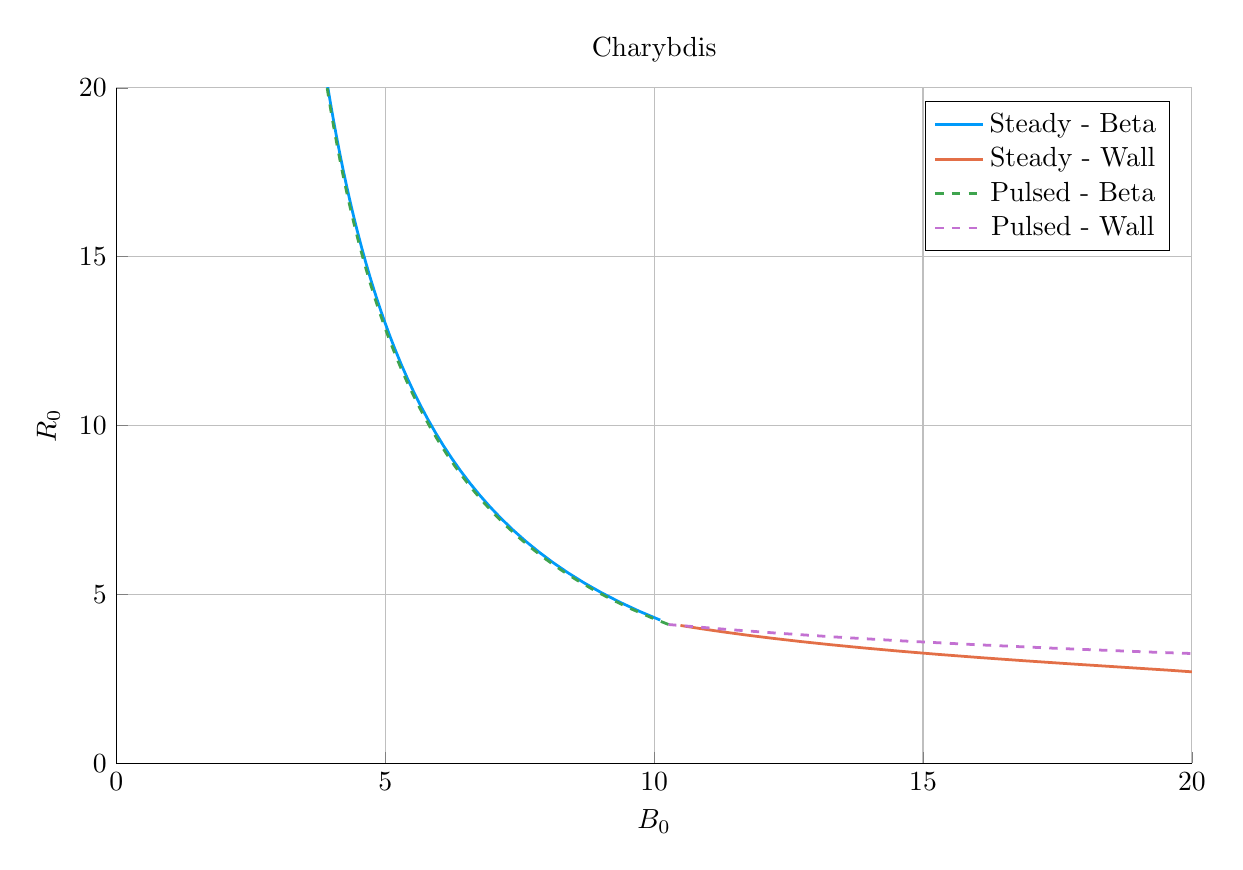
\begin{tikzpicture}[]
\begin{axis}[height = {101.6mm}, ylabel = {${R}_{0}$}, title = {Charybdis}, xmin = {0.0}, xmax = {20.0}, ymax = {20.0}, xlabel = {${B}_{0}$}, {unbounded coords=jump, scaled x ticks = false, xticklabel style={rotate = 0}, xmajorgrids = true, xtick = {0.0,5.0,10.0,15.0,20.0}, xticklabels = {0,5,10,15,20}, xtick align = inside, axis lines* = left, scaled y ticks = false, yticklabel style={rotate = 0}, ymajorgrids = true, ytick = {0.0,5.0,10.0,15.0,20.0}, yticklabels = {0,5,10,15,20}, ytick align = inside, axis lines* = left,     xshift = 0.0mm,
    yshift = 0.0mm,
    axis background/.style={fill={rgb,1:red,1.00000000;green,1.00000000;blue,1.00000000}}
, colorbar style={title=}}, ymin = {0.0}, width = {152.4mm}]\addplot+ [color = {rgb,1:red,0.00000000;green,0.60560316;blue,0.97868012},
draw opacity=1.0,
line width=1,
solid,mark = none,
mark size = 2.0,
mark options = {
    color = {rgb,1:red,0.00000000;green,0.00000000;blue,0.00000000}, draw opacity = 1.0,
    fill = {rgb,1:red,0.00000000;green,0.60560316;blue,0.97868012}, fill opacity = 1.0,
    line width = 1,
    rotate = 0,
    solid
}]coordinates {
(10.112818033153026, 4.241771689478311)
(9.722156888543116, 4.504138117525138)
(9.357875603858393, 4.77497367032698)
(9.017653755630063, 5.054228410858618)
(8.6995124437054, 5.34178832481448)
(8.401566530516865, 5.637594610921002)
(8.122163706328223, 5.941556970897918)
(7.859819415455661, 6.2535750482800845)
(7.613196557650265, 6.5735387749268055)
(7.381088038653343, 6.901328733442317)
(7.162401716104116, 7.236816533350192)
(6.956147367527331, 7.579865198961832)
(6.761425371986388, 7.930329566972662)
(6.577416849463348, 8.28805669191591)
(6.403375044688587, 8.652886257700402)
(6.2386177769852695, 9.02465099355178)
(6.0825208065966905, 9.403177092267818)
(5.934511989185341, 9.788284632344096)
(5.794066116682695, 10.179787994954152)
(5.660700347012839, 10.577496284633074)
(5.533970150598111, 10.981213744847159)
(5.413465705416883, 11.390740170754555)
(5.298808685607224, 11.805871315185586)
(5.189649392059402, 12.226399293085946)
(5.085664187259174, 12.652112975136994)
(4.986553195072601, 13.082798376170517)
(4.892038235455667, 13.518239035062717)
(4.801860966679364, 13.958216385902286)
(4.7157812114040425, 14.402510119861804)
(4.633575445956479, 14.850898537267405)
(4.5550354347559185, 15.303158889428241)
(4.479966994069385, 15.759067709846747)
(4.408188871204256, 16.21840113449116)
(4.33953172691477, 16.680935210866018)
(4.273837210246432, 17.14644619566822)
(4.210957116299974, 17.614710840865197)
(4.15075261849161, 18.085506668079862)
(4.0930935678432965, 18.558612231207235)
(4.037857852672517, 19.03380736722975)
(3.9849308127842145, 19.510873435234036)
(3.9342047029103653, 19.98959354366903)
(3.8855782007091695, 20.46975276591405)
(3.838955955133626, 20.951138344257103)
(3.7942481714200484, 21.433539882408354)
(3.7513702293348077, 21.91674952670236)
(3.710242331663442, 22.400562136158193)
(3.6707891802306123, 22.88477544159215)
(3.6329396770109583, 23.369190193993973)
(3.5966266481325166, 23.853610302391182)
(3.5617865887889004, 24.33784296144382)
(3.5283594272686503, 24.821698769019683)
(3.496288306480746, 25.30499183401733)
(3.465519381509793, 25.787539874702443)
(3.4360016318699595, 26.2691643078435)
(3.4076866872513096, 26.74969032892794)
(3.380528665662031, 27.228946983749)
(3.3544840229690007, 27.706767231660894)
(3.3295114129297314, 28.18298800079238)
(3.3055715568879336, 28.6574502355218)
(3.2826271223788512, 29.129998936506894)
(3.260642607548369, 29.600483215419466)
(3.239584247604666, 30.068756211731234)
(3.2194198921826622, 30.53467533068977)
(3.2001189373344725, 30.998102038032528)
(3.181652227422265, 31.45890197647381)
(3.163991977015565, 31.916944945395528)
(3.1471116955378684, 32.37210489697581)
(3.130986116696265, 32.82425992717794)
(3.115591132350856, 33.27329226186858)
(3.1009037305081053, 33.719088238329654)
(3.0869019371473265, 34.16153828242195)
(3.0735647616124355, 34.600536881650775)
(3.0608721453218655, 35.035982554380354)
};
\addlegendentry{Steady - Beta}
\addplot+ [color = {rgb,1:red,0.88887350;green,0.43564919;blue,0.27812294},
draw opacity=1.0,
line width=1,
solid,mark = none,
mark size = 2.0,
mark options = {
    color = {rgb,1:red,0.00000000;green,0.00000000;blue,0.00000000}, draw opacity = 1.0,
    fill = {rgb,1:red,0.88887350;green,0.43564919;blue,0.27812294}, fill opacity = 1.0,
    line width = 1,
    rotate = 0,
    solid
}]coordinates {
(20.758867641064707, 2.5885674971573294)
(20.346250098246923, 2.6701608818805265)
(19.57104597888471, 2.7580768645580767)
(18.681781921115476, 2.84914579801761)
(17.775790175980152, 2.942053074257325)
(16.896654716492492, 3.036102404206255)
(16.063927450323227, 3.1308756359103893)
(15.285557510665852, 3.226095678435203)
(14.563500533069154, 3.3215674678202314)
(13.896568848875791, 3.417147967307318)
(13.281970890030232, 3.5127292434426214)
(12.716170469467318, 3.6082281475654683)
(12.195372283741088, 3.7035796419955296)
(11.715794270833433, 3.798732281084355)
(11.273815669498969, 3.8936450383948094)
(10.866051794088186, 3.9882850129983627)
(10.489365023931143, 4.08262666943062)
};
\addlegendentry{Steady - Wall}
\addplot+ [color = {rgb,1:red,0.24222430;green,0.64327509;blue,0.30444865},
draw opacity=1.0,
line width=1,
dashed,mark = none,
mark size = 2.0,
mark options = {
    color = {rgb,1:red,0.00000000;green,0.00000000;blue,0.00000000}, draw opacity = 1.0,
    fill = {rgb,1:red,0.24222430;green,0.64327509;blue,0.30444865}, fill opacity = 1.0,
    line width = 1,
    rotate = 0,
    solid
}]coordinates {
(10.26788634689966, 4.1112515557786775)
(9.953967652326213, 4.3094639978912825)
(9.567926244368271, 4.576742787082168)
(9.207974394987358, 4.852707848855866)
(8.871841888699304, 5.137296446755483)
(8.557505525932248, 5.430432251844937)
(8.263156925406376, 5.732025498645217)
(7.9871752024348766, 6.041973183885721)
(7.728103682045175, 6.3601593098028015)
(7.484629973620137, 6.686455168691173)
(7.255568856523303, 7.020719666856628)
(7.039847526735421, 7.362799685753208)
(6.836492834698909, 7.712530477959993)
(6.644620209081183, 8.06973609553486)
(6.463424013335149, 8.43422984818008)
(6.2921691243175495, 8.80581478856818)
(6.13018355681404, 9.184284222105854)
(5.97685198655569, 9.569422237740964)
(5.831610044919842, 9.961004260702955)
(5.693939286027163, 10.358797615092055)
(5.563362729090489, 10.762562105803609)
(5.439440906144732, 11.172050607751359)
(5.321768347746793, 11.587009663771289)
(5.209970453003084, 12.007180084871303)
(5.103700692769835, 12.43229755779498)
(5.002638109938164, 12.862093246958203)
(4.906485077678376, 13.296294396161224)
(4.814965286571576, 13.734624924501638)
(4.727821933804548, 14.176806014771396)
(4.644816091323922, 14.622556692215932)
(4.565725232806084, 15.071594391671503)
(4.490341901840154, 15.523635511246878)
(4.418472505906755, 15.978395950871612)
(4.349936222622964, 16.435591634187325)
(4.284564006352339, 16.89493901242702)
(4.222197684694192, 17.3561555490841)
(4.162689135592264, 17.818960184341037)
(4.105899536872315, 18.283073778386605)
(4.051698680949713, 18.748219532911282)
(3.9999643482627323, 19.214123390225897)
(3.9505817337017928, 19.680514409594025)
(3.903442920928527, 20.147125120523665)
(3.858446400032002, 20.613691852887264)
(3.8154966244515616, 21.079955043879853)
(3.7745036035252744, 21.545659521938795)
(3.7353825273991994, 22.010554767868463)
(3.6980534213689746, 22.47439515350876)
(3.6624408270205375, 22.936940158387063)
(3.62847350780097, 23.397954564874027)
(3.5960841768845415, 23.85720863243935)
(3.565209245407392, 24.314478251672824)
(3.5357885893311605, 24.769545078785413)
(3.5077653333614305, 25.22219665136009)
(3.4810856504959875, 25.672226486155235)
(3.4556985759109375, 26.119434159797105)
(3.4315558340122845, 26.563625373217942)
(3.408611677587535, 27.004612000714285)
(3.3868227380888998, 27.44221212450356)
(3.36614788616562, 27.876250055664674)
(3.3465481016421226, 28.306556342336567)
(3.327986352208224, 28.732967766047434)
(3.3104274769652595, 29.155327355093103)
(3.2938380965241474, 29.573484219331384)
(3.278186482171801, 29.987293796610192)
(3.263442495132517, 30.396617529277517)
(3.2495774839156075, 30.801322953869263)
(3.236564206241785, 31.2012836153002)
(3.224376752844934, 31.596379002720997)
(3.212990475972638, 31.98649447963656)
(3.2023819222517877, 32.371521208907616)
(3.192528769611062, 32.751356073231776)
(3.1834097679780142, 33.12590159165121)
(3.1750046834890777, 33.49506583261046)
(3.1672942459724482, 33.8587623240416)
};
\addlegendentry{Pulsed - Beta}
\addplot+ [color = {rgb,1:red,0.76444018;green,0.44411178;blue,0.82429754},
draw opacity=1.0,
line width=1,
dashed,mark = none,
mark size = 2.0,
mark options = {
    color = {rgb,1:red,0.00000000;green,0.00000000;blue,0.00000000}, draw opacity = 1.0,
    fill = {rgb,1:red,0.76444018;green,0.44411178;blue,0.82429754}, fill opacity = 1.0,
    line width = 1,
    rotate = 0,
    solid
}]coordinates {
(48.990476413653056, 2.408463256282958)
(42.83950920694117, 2.5157944044289065)
(37.687790427214495, 2.623911121514849)
(33.33937742845888, 2.732773154793489)
(29.64296398154308, 2.8423415573543895)
(26.48039367255613, 2.9525785265823425)
(23.758442882319894, 3.0634472709719978)
(21.402860298405816, 3.174911900538905)
(19.353987387634486, 3.2869373368800954)
(17.563502020363714, 3.3994892396762393)
(15.991970371213752, 3.512533946790301)
(14.606987499719377, 3.6260384258753686)
(13.381751501116137, 3.7399702354868722)
(12.293960329570087, 3.854297494171075)
(11.32495111804522, 3.9689888562032056)
(10.459023415380802, 4.084013492866982)
(10.26788634689966, 4.1112515557786775)
};
\addlegendentry{Pulsed - Wall}
\end{axis}

\end{tikzpicture}

    \end{adjustbox}
        \caption{Charybdis Reactor}
    \end{subfigure}
    \hfill
    \begin{subfigure}[t]{0.45\textwidth}
        \centering
    \begin{adjustbox}{width=\textwidth}
      \Large
      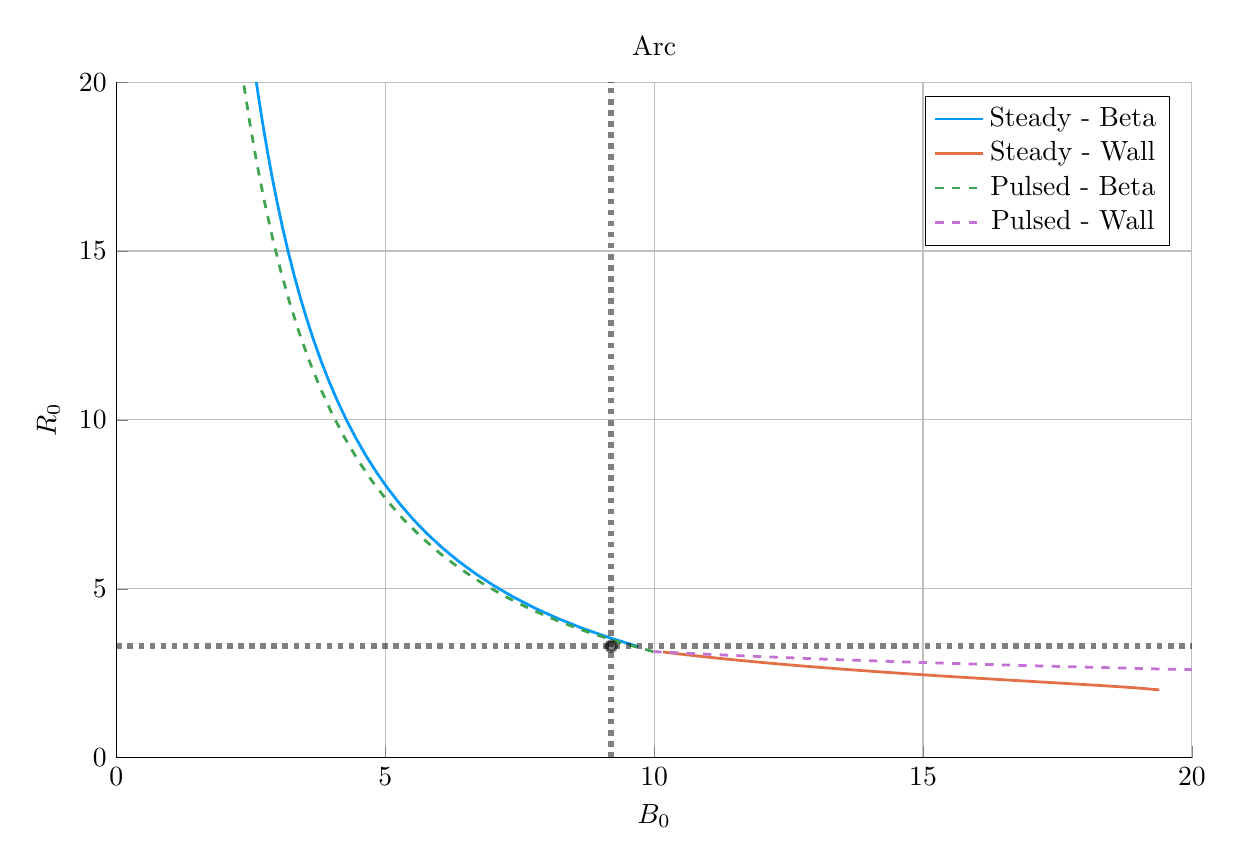
\begin{tikzpicture}[]
\begin{axis}[height = {101.6mm}, ylabel = {${R}_{0}$}, title = {Arc}, xmin = {0.0}, xmax = {20.0}, ymax = {20.0}, xlabel = {${B}_{0}$}, {unbounded coords=jump, scaled x ticks = false, xticklabel style={rotate = 0}, xmajorgrids = true, xtick = {0.0,5.0,10.0,15.0,20.0}, xticklabels = {0,5,10,15,20}, xtick align = inside, axis lines* = left, scaled y ticks = false, yticklabel style={rotate = 0}, ymajorgrids = true, ytick = {0.0,5.0,10.0,15.0,20.0}, yticklabels = {0,5,10,15,20}, ytick align = inside, axis lines* = left,     xshift = 0.0mm,
    yshift = 0.0mm,
    axis background/.style={fill={rgb,1:red,1.00000000;green,1.00000000;blue,1.00000000}}
, colorbar style={title=}}, ymin = {0.0}, width = {152.4mm}]\addplot+ [color = {rgb,1:red,0.00000000;green,0.60560316;blue,0.97868012},
draw opacity=1.0,
line width=1,
solid,mark = none,
mark size = 2.0,
mark options = {
    color = {rgb,1:red,0.00000000;green,0.00000000;blue,0.00000000}, draw opacity = 1.0,
    fill = {rgb,1:red,0.00000000;green,0.60560316;blue,0.97868012}, fill opacity = 1.0,
    line width = 1,
    rotate = 0,
    solid
}]coordinates {
(9.701206080853105, 3.2904233285656006)
(9.162315904693079, 3.553631706046861)
(8.664301107137337, 3.8315748016260343)
(8.203576462497304, 4.124583886864978)
(7.776718537485166, 4.433072975674755)
(7.380720231870917, 4.75741949036414)
(7.012886014999712, 5.097987291342331)
(6.670795005901889, 5.4551257000070565)
(6.352268997292712, 5.829168567645448)
(6.055344682097163, 6.220433393277178)
(5.778249464564785, 6.629220493040615)
(5.519380338856715, 7.05581222339423)
(5.2772854007125325, 7.500472260074458)
(5.050647625972996, 7.963444934423652)
(4.838270606140816, 8.444954628380609)
(4.639065978019038, 8.94520522910952)
(4.4520423235376105, 9.464379643936518)
(4.276295348572609, 10.002639375969222)
(4.110999177018484, 10.56012416048812)
(3.9553986195015125, 11.136951661929974)
(3.8088022956698633, 11.733217231026282)
(3.6705765055641186, 12.34899372141899)
(3.54013975965751, 12.984331364849716)
(3.4169578891619192, 13.639257703809928)
(3.30053966845824, 14.313777580345645)
(3.1904328903033052, 15.007873179535935)
(3.086220842019516, 15.721504126002731)
(2.9875191373772063, 16.45460763166718)
(2.8939728644914635, 17.207098692842226)
(2.8052540149097247, 17.97887033463821)
(2.7210591632720242, 18.7697939005645)
(2.6411073705789065, 19.579719385129263)
(2.565138287279709, 20.40847580717446)
(2.492910435164382, 21.255871621630877)
(2.4241996494611984, 22.12169516733927)
(2.3587976646588236, 23.0057151485579)
(2.296510829425685, 23.907681147764652)
(2.237158937627476, 24.827324167354146)
(2.180574163874242, 25.764357197843207)
(2.126600093288366, 26.71847581021091)
(2.075090836295778, 27.689358770027713)
(2.0259102202234582, 28.676668671060817)
(1.978931050353818, 29.68005258608471)
(1.9340344338545452, 30.69914273267572)
(1.8911091606836798, 31.733557151818793)
(1.8500511361739687, 32.78290039722107)
(1.8107628605384507, 33.846764233283025)
(1.773152951016952, 34.92472833975579)
(1.7371357028100902, 36.01636102117257)
(1.7026306853269466, 37.121219919229354)
(1.6695623706125668, 38.23885272635799)
(1.6378597911249178, 39.368797898817405)
(1.607456224302725, 40.51058536770822)
(1.5782889016090462, 41.663737246396295)
(1.5502987399539199, 42.82776853291479)
(1.5234300935954943, 44.00218780599217)
(1.4976305247952577, 45.18649791343829)
(1.4728505916614916, 46.38019665170201)
(1.4490436517578602, 47.58277743549339)
(1.4261656801829077, 48.79372995643627)
};
\addlegendentry{Steady - Beta}
\addplot+ [color = {rgb,1:red,0.88887350;green,0.43564919;blue,0.27812294},
draw opacity=1.0,
line width=1,
solid,mark = none,
mark size = 2.0,
mark options = {
    color = {rgb,1:red,0.00000000;green,0.00000000;blue,0.00000000}, draw opacity = 1.0,
    fill = {rgb,1:red,0.88887350;green,0.43564919;blue,0.27812294}, fill opacity = 1.0,
    line width = 1,
    rotate = 0,
    solid
}]coordinates {
(19.394007482712425, 2.006855814841082)
(18.932196567189358, 2.070220226465634)
(18.296989378345195, 2.1362327099649083)
(17.587029315408756, 2.2039322514902886)
(16.847882407994106, 2.272885741349308)
(16.111374502564406, 2.3427307443133163)
(15.396027314547156, 2.4132115621474344)
(14.710952688793137, 2.484165095168367)
(14.06168447794857, 2.555449485048069)
(13.450465418483889, 2.6269568263788754)
(12.877644538645335, 2.6986005527245354)
(12.342394470642008, 2.7703103261458715)
(11.843182246608265, 2.8420284550528074)
(11.376441269625893, 2.9137564749008216)
(10.944966372727551, 2.985307257194073)
(10.541663878705513, 3.056795384934831)
(10.165908182236457, 3.128148092221394)
};
\addlegendentry{Steady - Wall}
\addplot+ [color = {rgb,1:red,0.24222430;green,0.64327509;blue,0.30444865},
draw opacity=1.0,
line width=1,
dashed,mark = none,
mark size = 2.0,
mark options = {
    color = {rgb,1:red,0.00000000;green,0.00000000;blue,0.00000000}, draw opacity = 1.0,
    fill = {rgb,1:red,0.24222430;green,0.64327509;blue,0.30444865}, fill opacity = 1.0,
    line width = 1,
    rotate = 0,
    solid
}]coordinates {
(9.980483622051658, 3.1402982942956537)
(9.392786903460065, 3.3984668375583613)
(8.79273598103983, 3.7029994270206985)
(8.23820290909994, 4.029752381934837)
(7.725182218401588, 4.380005330007902)
(7.250078106370205, 4.755088191072525)
(6.80965553466646, 5.15638156809462)
(6.400998063035608, 5.585317075247801)
(6.0214713600430425, 6.043377623224966)
(5.668691517461799, 6.532097691007738)
(5.340497445229901, 7.053063624618788)
(5.034926745580058, 7.607914017422467)
(4.750194564008521, 8.198340243900201)
(4.484674995755211, 8.826087240213646)
(4.236884692979903, 9.49295465115087)
(4.00546837264544, 10.200798495308337)
(3.7891859704718387, 10.951533539957822)
(3.5869012239550364, 11.747136625739826)
(3.3975714987448393, 12.589651241396528)
(3.2202386987489797, 13.481193723261853)
(3.0540211220494466, 14.423961547290066)
(2.8981061427709687, 15.420244298711943)
(2.7517436139566023, 16.472438053930638)
(2.6142398986781377, 17.58306410230943)
(2.4849524463010138, 18.754793188384546)
(2.363284838174807, 19.990476791576892)
(2.248682232019848, 21.293187416028662)
(2.140627136740878, 22.666270490916787)
(2.038635448877246, 24.113411362836906)
(1.9422526775794744, 25.638722123308433)
(1.8510502754751532, 27.246854857488287)
(1.7646219756564088, 28.94315065234289)
(1.6825800061969869, 30.73383791051506)
(1.6045510059627948, 32.62630011975996)
(1.53017138625397, 34.629443897654504)
(1.4590817483192686, 36.754215952550474)
(1.3909197311384796, 39.01434852880224)
(1.3253102336217724, 41.42746903285954)
(1.261851128383913, 44.01681696754988)
(1.20009089049112, 46.81403058684408)
(1.1394908096975784, 49.863950342519615)
};
\addlegendentry{Pulsed - Beta}
\addplot+ [color = {rgb,1:red,0.76444018;green,0.44411178;blue,0.82429754},
draw opacity=1.0,
line width=1,
dashed,mark = none,
mark size = 2.0,
mark options = {
    color = {rgb,1:red,0.00000000;green,0.00000000;blue,0.00000000}, draw opacity = 1.0,
    fill = {rgb,1:red,0.76444018;green,0.44411178;blue,0.82429754}, fill opacity = 1.0,
    line width = 1,
    rotate = 0,
    solid
}]coordinates {
(29.27715761652869, 2.3448804182939873)
(25.4410619834368, 2.4377937236066716)
(22.158819835998365, 2.5322208586485804)
(19.342453256965573, 2.628163744265164)
(16.919364280634177, 2.7256238396687067)
(14.829378672669455, 2.8246020951898183)
(13.022412368922526, 2.9250989082568273)
(11.456617692058645, 3.0271140820266207)
(10.096901921254785, 3.1306467862637533)
(9.980483622051658, 3.1402982942956537)
};
\addlegendentry{Pulsed - Wall}
\addplot+ [color = {rgb,1:red,0.00000000;green,0.00000000;blue,0.00000000},
draw opacity=0.5,
line width=2,
dotted,mark = none,
mark size = 2.0,
mark options = {
    color = {rgb,1:red,0.00000000;green,0.00000000;blue,0.00000000}, draw opacity = 0.5,
    fill = {rgb,1:red,0.00000000;green,0.00000000;blue,0.00000000}, fill opacity = 0.5,
    line width = 1,
    rotate = 0,
    solid
},forget plot]coordinates {
(0.0, 3.3)
(20.0, 3.3)
};
\addplot+ [color = {rgb,1:red,0.00000000;green,0.00000000;blue,0.00000000},
draw opacity=0.5,
line width=2,
dotted,mark = none,
mark size = 2.0,
mark options = {
    color = {rgb,1:red,0.00000000;green,0.00000000;blue,0.00000000}, draw opacity = 0.5,
    fill = {rgb,1:red,0.00000000;green,0.00000000;blue,0.00000000}, fill opacity = 0.5,
    line width = 1,
    rotate = 0,
    solid
},forget plot]coordinates {
(9.2, 0.0)
(9.2, 20.0)
};
\addplot+[draw=none, color = {rgb,1:red,0.00000000;green,0.00000000;blue,0.00000000},
draw opacity=0.5,
line width=0,
solid,mark = *,
mark size = 2.0,
mark options = {
    color = {rgb,1:red,0.00000000;green,0.00000000;blue,0.00000000}, draw opacity = 0.5,
    fill = {rgb,1:red,0.00000000;green,0.00000000;blue,0.00000000}, fill opacity = 0.5,
    line width = 1,
    rotate = 0,
    solid
},forget plot] coordinates {
(9.2, 3.3)
};
\end{axis}

\end{tikzpicture}

    \end{adjustbox}
        \caption{Arc Reactor}
    \end{subfigure}
    \hfill \hfill ~\\ ~\\ ~\\
    \caption{Steady State Prototype Comparison} ~\\
    \label{fig:charybdis}
\end{figure*}

\begin{table}[h!]
\centering  
\caption{Charybdis Variables}
\hfill
\begin{subtable}[t]{0.4\textwidth}
\centering  
\caption{Input Variables} ~\\
\begin{tabular}{ c|c } 

Input            & Value           \\
\hline
$H$              & 1.7              \\
$Q$              & 25.0             \\
$N_{G}$          & 0.9              \\
$\epsilon$       & 0.3              \\
$\kappa_{95}$    & 1.8              \\
$\delta_{95}$    & 0.35             \\
$\nu_{n}$        & 0.4              \\
$\nu_{T}$        & 1.1              \\
$l_{i}$          & 0.5579         \\
$A$              & 2.5              \\
$Z_{eff}$        & 1.75             \\
$f_{D}$          & 0.9              \\
$\tau_{FT}$      & 1.6e9            \\
$B_{CS}$         & 12.0             \\

\end{tabular}
\end{subtable}
\hfill
\begin{subtable}[t]{0.5\textwidth}
\centering  
\caption{Output Variables} ~\\
\begin{tabular}{ c|c } 

Output           & Value       \\
\hline
$R_{0}$          & 4.13            \\
$B_{0}$          & 10.28            \\
$I_{P}$          & 8.98            \\
$\overline n$    & 1.47            \\
$\overline T$    & 15.81           \\
$\beta_{N}$       & 0.028            \\
$q_{95}$         & 6.089            \\
$P_{W}$          & 3.003            \\
$f_{BS}$         & 0.723           \\
$f_{CD}$         & 0.277           \\
$f_{IN}$         & 0.0              \\
$\volume$         & 225.5            \\
$P_{F}$          & 1294           \\
$\eta_{CD}$      & 0.291           \\

\end{tabular}
\end{subtable}
\hfill
\hfill
\end{table}

\newpage 

\subsection{Pinning down Proteus}

The pulsed twin reactor, Proteus, highlights the effects o f a high field central solenoid. When compared to the Pulsed Demo design, the $R_0$ -- $B_0$ curves look far more favorable -- i.e. each machine built at a certain magnet strength would be more compact (and cheaper). An interesting facet of Proteus is that it exhibits all three used limits: kink, beta, and wall.

\begin{figure*}[h!]
    \centering
    \hfill 
    \begin{subfigure}[t]{0.45\textwidth}
        \centering
    \begin{adjustbox}{width=\textwidth}
      \Large
      \begin{tikzpicture}[]
\begin{axis}[height = {101.6mm}, ylabel = {${R}_{0}$}, title = {Proteus}, xmin = {0.0}, xmax = {20.0}, ymax = {20.0}, xlabel = {${B}_{0}$}, {unbounded coords=jump, scaled x ticks = false, xticklabel style={rotate = 0}, xmajorgrids = true, xtick = {0.0,5.0,10.0,15.0,20.0}, xticklabels = {0,5,10,15,20}, xtick align = inside, axis lines* = left, scaled y ticks = false, yticklabel style={rotate = 0}, ymajorgrids = true, ytick = {0.0,5.0,10.0,15.0,20.0}, yticklabels = {0,5,10,15,20}, ytick align = inside, axis lines* = left,     xshift = 0.0mm,
    yshift = 0.0mm,
    axis background/.style={fill={rgb,1:red,1.00000000;green,1.00000000;blue,1.00000000}}
, colorbar style={title=}}, ymin = {0.0}, width = {152.4mm}]\addplot+ [color = {rgb,1:red,0.00000000;green,0.60560316;blue,0.97868012},
draw opacity=1.0,
line width=1,
solid,mark = none,
mark size = 2.0,
mark options = {
    color = {rgb,1:red,0.00000000;green,0.00000000;blue,0.00000000}, draw opacity = 1.0,
    fill = {rgb,1:red,0.00000000;green,0.60560316;blue,0.97868012}, fill opacity = 1.0,
    line width = 1,
    rotate = 0,
    solid
}]coordinates {
(4.658732060637907, 15.19267920719026)
(4.211109766361548, 13.257359890602805)
(3.9293920326356777, 11.874737313931622)
(3.7651903683456465, 10.866007699416029)
(3.6776039543745567, 10.103021459180615)
(3.6402437753208394, 9.505760636119051)
(3.6366994671255806, 9.024418756735512)
(3.656621534643579, 8.627122931627166)
(3.693300156736026, 8.29276379316033)
(3.7422515017241134, 8.006879676976913)
(3.865532743079537, 7.5424484228595015)
(3.936096932264377, 7.350942552250971)
(4.010907188015084, 7.180521653028847)
(4.089072356933184, 7.027918062531758)
(4.169903401491354, 6.8905526178616)
(4.252857906625248, 6.7663586425757165)
(4.337501757261618, 6.653657691692545)
(4.42348218754058, 6.551070097987566)
(4.5983381267510195, 6.371833566535418)
(4.686766232902671, 6.29340795554276)
(4.775618142770625, 6.221477142908907)
(4.864743502376605, 6.155442914152805)
(4.927312314219091, 6.1123879686673135)
};
\addlegendentry{Pulsed - Kink}
\addplot+ [color = {rgb,1:red,0.88887350;green,0.43564919;blue,0.27812294},
draw opacity=1.0,
line width=1,
solid,mark = none,
mark size = 2.0,
mark options = {
    color = {rgb,1:red,0.00000000;green,0.00000000;blue,0.00000000}, draw opacity = 1.0,
    fill = {rgb,1:red,0.88887350;green,0.43564919;blue,0.27812294}, fill opacity = 1.0,
    line width = 1,
    rotate = 0,
    solid
}]coordinates {
(4.927312314219091, 6.1123879686673135)
(4.984545814413324, 6.09581207033949)
(5.17452482724068, 6.0447147858623)
(5.362091669637646, 5.999934523234248)
(5.54700293215903, 5.961033646850443)
(5.729042482638278, 5.92761240871646)
(5.908022832274664, 5.899302777254819)
(6.083785777786694, 5.87576371038825)
(6.256202341425288, 5.85667756374391)
(6.324169421042356, 5.850226299362774)
};
\addlegendentry{Pulsed - Beta}
\addplot+ [color = {rgb,1:red,0.24222430;green,0.64327509;blue,0.30444865},
draw opacity=1.0,
line width=1,
solid,mark = none,
mark size = 2.0,
mark options = {
    color = {rgb,1:red,0.00000000;green,0.00000000;blue,0.00000000}, draw opacity = 1.0,
    fill = {rgb,1:red,0.24222430;green,0.64327509;blue,0.30444865}, fill opacity = 1.0,
    line width = 1,
    rotate = 0,
    solid
}]coordinates {
(6.324169421042356, 5.850226299362774)
(6.727338549778396, 5.88388315153579)
(7.320469048424473, 5.950696360836003)
(7.835746509376305, 6.026778469060774)
(8.290245520072391, 6.109137751468495)
(8.696162676727877, 6.195913809142839)
(9.0624397222742, 6.285887257774413)
(9.395798186463841, 6.3782240354403505)
(9.701405747258567, 6.472333393687546)
(10.244760202900984, 6.664256338261126)
(10.930275827723788, 6.957604003970967)
(11.131878682735255, 7.056189303396245)
(11.50278450645086, 7.253945523825199)
(11.83715172742864, 7.452031096358636)
(11.992609772603878, 7.551070724623068)
(12.141110720831467, 7.650057379146056)
};
\addlegendentry{Pulsed - Wall}
\end{axis}

\end{tikzpicture}

    \end{adjustbox}
        \caption{Proteus Reactor}
    \end{subfigure}
    \hfill
    \begin{subfigure}[t]{0.45\textwidth}
        \centering
    \begin{adjustbox}{width=\textwidth}
      \Large
      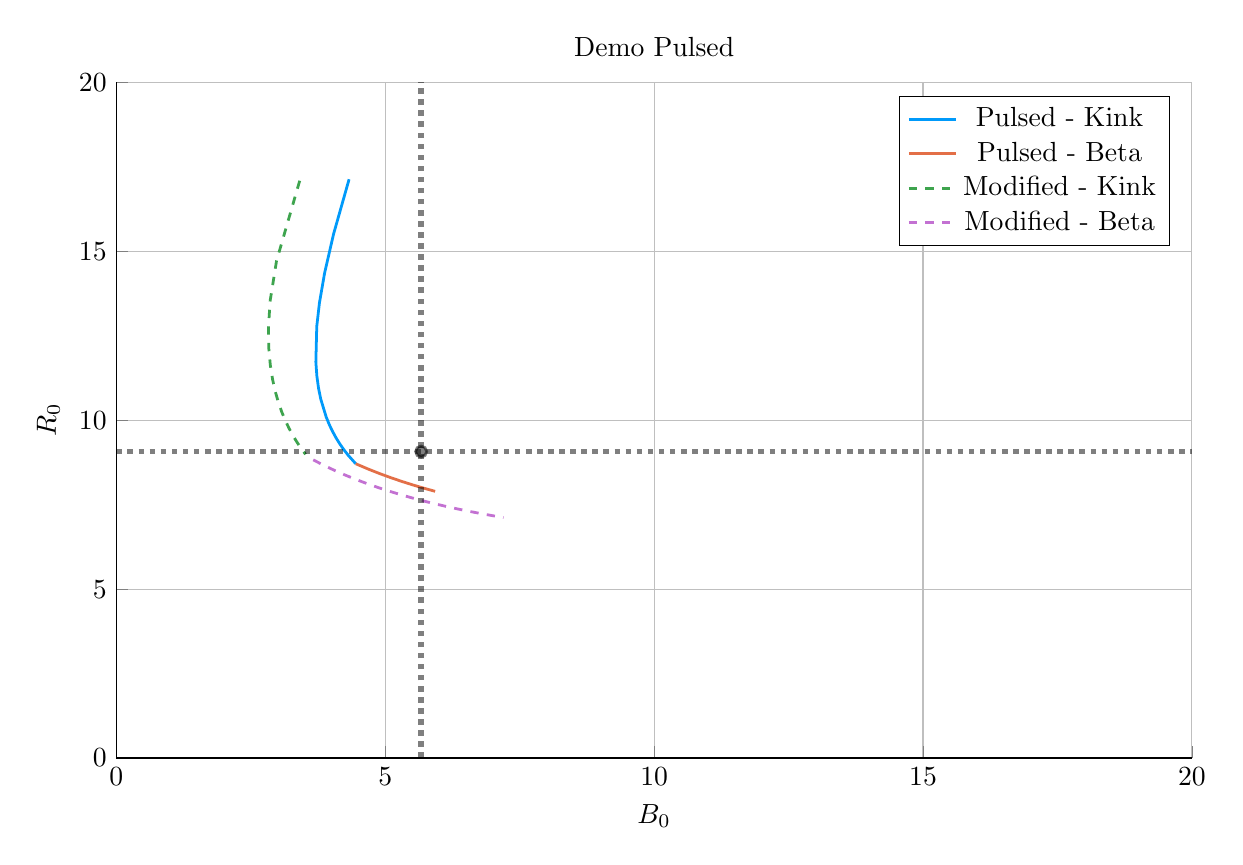
\begin{tikzpicture}[]
\begin{axis}[height = {101.6mm}, ylabel = {${R}_{0}$}, title = {Demo Pulsed}, xmin = {0.0}, xmax = {20.0}, ymax = {20.0}, xlabel = {${B}_{0}$}, {unbounded coords=jump, scaled x ticks = false, xticklabel style={rotate = 0}, xmajorgrids = true, xtick = {0.0,5.0,10.0,15.0,20.0}, xticklabels = {0,5,10,15,20}, xtick align = inside, axis lines* = left, scaled y ticks = false, yticklabel style={rotate = 0}, ymajorgrids = true, ytick = {0.0,5.0,10.0,15.0,20.0}, yticklabels = {0,5,10,15,20}, ytick align = inside, axis lines* = left,     xshift = 0.0mm,
    yshift = 0.0mm,
    axis background/.style={fill={rgb,1:red,1.00000000;green,1.00000000;blue,1.00000000}}
, colorbar style={title=}}, ymin = {0.0}, width = {152.4mm}]\addplot+ [color = {rgb,1:red,0.00000000;green,0.60560316;blue,0.97868012},
draw opacity=1.0,
line width=1,
solid,mark = none,
mark size = 2.0,
mark options = {
    color = {rgb,1:red,0.00000000;green,0.00000000;blue,0.00000000}, draw opacity = 1.0,
    fill = {rgb,1:red,0.00000000;green,0.60560316;blue,0.97868012}, fill opacity = 1.0,
    line width = 1,
    rotate = 0,
    solid
}]coordinates {
(4.327031075670194, 17.134796748649162)
(4.038214026054326, 15.511755022601415)
(3.8713719163129245, 14.355562963913712)
(3.7758613845615545, 13.476675762289453)
(3.7257856761317214, 12.778294295391971)
(3.7090473695925437, 11.723065749829066)
(3.727711597554826, 11.30970201784727)
(3.7586131667481433, 10.94971275897184)
(3.799052518631718, 10.632190690377048)
(3.901290136389271, 10.09455415135144)
(3.960577465316514, 9.863813619410237)
(4.0241209645210345, 9.653307397969705)
(4.0912717805663785, 9.460162902699798)
(4.161514602943343, 9.28206292757184)
(4.2344343960723005, 9.117114543572253)
(4.309692554546368, 8.963753917462126)
(4.450417240491067, 8.712493965092264)
};
\addlegendentry{Pulsed - Kink}
\addplot+ [color = {rgb,1:red,0.88887350;green,0.43564919;blue,0.27812294},
draw opacity=1.0,
line width=1,
solid,mark = none,
mark size = 2.0,
mark options = {
    color = {rgb,1:red,0.00000000;green,0.00000000;blue,0.00000000}, draw opacity = 1.0,
    fill = {rgb,1:red,0.88887350;green,0.43564919;blue,0.27812294}, fill opacity = 1.0,
    line width = 1,
    rotate = 0,
    solid
}]coordinates {
(4.450417240491067, 8.712493965092264)
(4.490148631384312, 8.684308742646298)
(4.692490181445514, 8.547262773806349)
(4.8960344619053355, 8.41947837460442)
(5.100651132702229, 8.30014929484307)
(5.306202822090688, 8.188581738801314)
(5.512545696627038, 8.084175191078112)
(5.719530043226767, 7.986407002697611)
(5.927000883375481, 7.894819882619234)
};
\addlegendentry{Pulsed - Beta}
\addplot+ [color = {rgb,1:red,0.24222430;green,0.64327509;blue,0.30444865},
draw opacity=1.0,
line width=1,
dashed,mark = none,
mark size = 2.0,
mark options = {
    color = {rgb,1:red,0.00000000;green,0.00000000;blue,0.00000000}, draw opacity = 1.0,
    fill = {rgb,1:red,0.24222430;green,0.64327509;blue,0.30444865}, fill opacity = 1.0,
    line width = 1,
    rotate = 0,
    solid
}]coordinates {
(3.4087424183072135, 17.090884129081292)
(2.977074181068944, 14.713048632784332)
(2.8592500074202523, 13.541171522519205)
(2.827199220063259, 12.740024138753894)
(2.8339789008667826, 12.12574468151967)
(2.862412302880871, 11.626187613249266)
(2.9044598258085443, 11.205091848948229)
(2.95577893007882, 10.841432203317366)
(3.0137895352525907, 10.521822649209419)
(3.076849710218805, 10.23716073884787)
(3.1438583711612704, 9.980947801083442)
(3.214045733980633, 9.748367275345563)
(3.2868548955983727, 9.535742205343247)
(3.361871149981842, 9.340197658526863)
(3.4387778750377818, 9.15944098345979)
(3.5173279629378453, 8.991613349767409)
};
\addlegendentry{Modified - Kink}
\addplot+ [color = {rgb,1:red,0.76444018;green,0.44411178;blue,0.82429754},
draw opacity=1.0,
line width=1,
dashed,mark = none,
mark size = 2.0,
mark options = {
    color = {rgb,1:red,0.00000000;green,0.00000000;blue,0.00000000}, draw opacity = 1.0,
    fill = {rgb,1:red,0.76444018;green,0.44411178;blue,0.82429754}, fill opacity = 1.0,
    line width = 1,
    rotate = 0,
    solid
}]coordinates {
(3.6607028750648505, 8.825949645171955)
(3.8574448036470477, 8.664618827122876)
(4.056375867871351, 8.51434867582932)
(4.257366397480293, 8.374075613831488)
(4.460279103534801, 8.242896218794312)
(4.664969389370631, 8.12003771613466)
(4.871285596007394, 8.004834914067093)
(5.07906923307514, 7.896711937521184)
(5.288155233306219, 7.795167587687744)
(5.498372259673351, 7.699763475973523)
(5.709543087166185, 7.610114306522102)
(5.921485076209294, 7.525879840414137)
(6.134010749367255, 7.446758190646709)
(6.346928478632384, 7.372480180910637)
(6.560043285872518, 7.302804563889649)
(6.773157754368795, 7.237513941672651)
(6.986073044284746, 7.176411266758267)
(7.198590001107076, 7.119316828230052)
};
\addlegendentry{Modified - Beta}
\addplot+ [color = {rgb,1:red,0.00000000;green,0.00000000;blue,0.00000000},
draw opacity=0.5,
line width=2,
dotted,mark = none,
mark size = 2.0,
mark options = {
    color = {rgb,1:red,0.00000000;green,0.00000000;blue,0.00000000}, draw opacity = 0.5,
    fill = {rgb,1:red,0.00000000;green,0.00000000;blue,0.00000000}, fill opacity = 0.5,
    line width = 1,
    rotate = 0,
    solid
},forget plot]coordinates {
(0.0, 9.072)
(20.0, 9.072)
};
\addplot+ [color = {rgb,1:red,0.00000000;green,0.00000000;blue,0.00000000},
draw opacity=0.5,
line width=2,
dotted,mark = none,
mark size = 2.0,
mark options = {
    color = {rgb,1:red,0.00000000;green,0.00000000;blue,0.00000000}, draw opacity = 0.5,
    fill = {rgb,1:red,0.00000000;green,0.00000000;blue,0.00000000}, fill opacity = 0.5,
    line width = 1,
    rotate = 0,
    solid
},forget plot]coordinates {
(5.667, 0.0)
(5.667, 20.0)
};
\addplot+[draw=none, color = {rgb,1:red,0.00000000;green,0.00000000;blue,0.00000000},
draw opacity=0.5,
line width=0,
solid,mark = *,
mark size = 2.0,
mark options = {
    color = {rgb,1:red,0.00000000;green,0.00000000;blue,0.00000000}, draw opacity = 0.5,
    fill = {rgb,1:red,0.00000000;green,0.00000000;blue,0.00000000}, fill opacity = 0.5,
    line width = 1,
    rotate = 0,
    solid
},forget plot] coordinates {
(5.667, 9.072)
};
\end{axis}

\end{tikzpicture}

    \end{adjustbox}
        \caption{Demo Pulsed Reactor}
    \end{subfigure}
    \hfill \hfill ~\\ ~\\ ~\\
    \caption{Pulsed Prototype Comparison} ~\\
\end{figure*}

\begin{table}[h!]
\centering  
\caption{Proteus Variables}
\hfill
\begin{subtable}[t]{0.4\textwidth}
\centering  
\caption{Input Variables} ~\\
\begin{tabular}{ c|c } 

Input            & Value           \\
\hline
$H$              & 1.0              \\
$Q$              & 25.0             \\
$N_{G}$          & 0.9              \\
$\epsilon$       & 0.3              \\
$\kappa_{95}$    & 1.8              \\
$\delta_{95}$    & 0.35             \\
$\nu_{n}$        & 0.4              \\
$\nu_{T}$        & 1.1              \\
$l_{i}$          & 0.6328         \\
$A$              & 2.5              \\
$Z_{eff}$        & 1.75             \\
$f_{D}$          & 0.9              \\
$\tau_{FT}$      & 7200           \\
$B_{CS}$         & 20.0             \\

\end{tabular}
\end{subtable}
\hfill
\begin{subtable}[t]{0.5\textwidth}
\centering  
\caption{Output Variables} ~\\
\begin{tabular}{ c|c } 

Output           & Value       \\
\hline
$R_{0}$          & 6.11             \\
$B_{0}$          & 4.93            \\
$I_{P}$          & 15.54            \\
$\overline n$    & 1.16            \\
$\overline T$    & 11.25            \\
$\beta_{N}$       & 0.028            \\
$q_{95}$         & 2.5              \\
$P_{W}$          & 1.763            \\
$f_{BS}$         & 0.2675           \\
$f_{CD}$         & 0.0              \\
$f_{IN}$         & 0.7325           \\
$\volume$         & 732.6            \\
$P_{F}$          & 1667           \\
$\eta_{CD}$      & 0.0              \\

\end{tabular}
\end{subtable}
\hfill
\hfill
\end{table}

\section{Learning from the Data}

Now that the model has been properly vetted and prototypes designed, we can explore how pulsed and steady-state tokamaks scale. Fitting with the Dickens theme, there will be three mostly independent results. The first result will explore how to minimize costs for a reactor by choosing optimum design points. The next will be an argument for how to properly utilize the HTS magnet technology in component design. Lastly, we will take a cursory look at the other parameters capable of lowering machine costs.

%\end{document}
